% Definisikan tipe dokumen sebagai report dengan satu kolom.
\documentclass[12pt, a4paper, onecolumn, twoside, final]{report}
\raggedbottom

\usepackage[none]{hyphenat}
\usepackage{hyperref}
% Memuat konfigurasi LaTeX khusus karya tulis di UI.
\usepackage{_internals/uithesis}

\UseRawInputEncoding
% Memuat konfigurasi khusus untuk laporan yang sedang dibuat.
% Definisikan judul laporan dalam bahasa Indonesia dan Inggris.
\def\judul{Eksperimen \textit{End-to-End Kafka Topic Partitioning} dengan Algoritma BroMax dan BroMin}
\def\judulInggris{End-to-End Experiment on Kafka Topic Partitioning with BroMax and BroMin Algorithms}

% Tipe laporan, misalnya: Laporan Kerja Praktik, Kampus Merdeka, Skripsi, Tugas Akhir, Thesis, atau Disertasi.
\def\type{Laporan Kerja Praktik}

% Jenjang studi penulis, bisa berisi: Diploma, Sarjana, Magister, atau Doktor.
\def\jenjang{Sarjana}

% Nama lengkap penulis laporan.
\def\penulisSatu{Bryan Raihan 'Ilman} % nama lengkap penulis pertama
\def\penulisDua{} % nama lengkap penulis kedua
\def\penulisTiga{} % nama lengkap penulis ketiga

% NPM untuk setiap penulis.
\def\npmSatu{2106704351} % NPM penulis pertama
\def\npmDua{} % NPM penulis kedua
\def\npmTiga{} % NPM penulis ketiga

% Program studi yang diambil oleh penulis.
\def\programSatu{Ilmu Komputer} % program studi penulis pertama
\def\programDua{} % program studi penulis kedua
\def\programTiga{} % program studi penulis ketiga

% Program studi dalam bahasa Inggris.
\def\studyProgramSatu{Computer Science} % 1st author's study program
\def\studyProgramDua{} % 2nd author's study program
\def\studyProgramTiga{} % 3rd author's study program

% Nama pembimbing dan penguji laporan.
\def\pembimbingSatu{Ichlasul Affan, M.Kom.}
\def\pembimbingDua{}
\def\pembimbingTiga{}

% Fakultas tempat penulis menempuh studi.
\def\fakultas{Ilmu Komputer}
\Var{\bulanTahun}{Agustus 2024}

% Gelar yang akan diperoleh setelah menyelesaikan laporan ini.
\def\gelar{Sarjana}
\def\tanggalLulus{25 Agustus 2024}

% Daftar judul bab pada laporan.
% Ubah judul sesuai dengan kebutuhan Anda.
\Var{\kataPengantar}{Kata Pengantar}
\Var{\babSatu}{Pendahuluan}
\Var{\babDua}{Isi}
\Var{\babTiga}{Penutup}
\Var{\babEmpat}{}
\Var{\babLima}{}
\Var{\kesimpulan}{}

% Jangan mengubah bagian di bawah ini.
\Var{\Judul}{\judul}
\Var{\Type}{\type}
\Var{\PenulisSatu}{\penulisSatu}
\Var{\PenulisDua}{\penulisDua}
\Var{\PenulisTiga}{\penulisTiga}
\Var{\Fakultas}{\fakultas}
\Var{\ProgramSatu}{\programSatu}
\Var{\ProgramDua}{\programDua}
\Var{\ProgramTiga}{\programTiga}

% Memuat daftar pemenggalan suku kata dan istilah dalam Bahasa Indonesia.
% Tambahkan cara pemenggalan kata-kata yang salah dipenggal secara otomatis oleh LaTeX.
% Jika kata tersebut dapat dipenggal dengan benar,
% maka tidak perlu ditambahkan dalam berkas ini.
% Tanda pemenggalan kata menggunakan tanda '-'; contoh:
% menarik
%   --> pemenggalan: me-na-rik
%


% Silakan ganti ke bahasa Inggris (\selectlanguage{english}) jika Anda merasa terlalu banyak kata bahasa Inggris yang pemenggalannya tidak benar.
%\selectlanguage{english}


\hyphenation{
    % alphabhet A
    a-na-li-sa a-tur a-tur-an
    a-pli-ka-si
    % alphabhet B
    bab ba-ngun-an
    be-be-ra-pa
    ber-ge-rak
    ber-ke-lan-jut-an
    ber-o-per-ra-si
    ber-pe-nga-ruh
    % alphabhet C
    ca-ri Com-po-nent-UML
    % alphabhet D
    di-da-pat-kan di-sim-pan di-pim-pin di-tam-bah-kan di-tem-pat-kan de-ngan da-e-rah di-ba-ngun di-gu-na-kan da-pat di-nya-ta-kan
    di-se-mat-kan di-sim-bol-kan di-pi-lih di-li-hat de-fi-ni-si di-de-fi-ni-si-kan di-mo-del-kan di-mi-li-ki di-re-a-li-sa-si-kan di-su-sun
    % alphabhet E
    eks-pli-sit e-ner-gi en-gi-neer en-gi-neer-ing eks-klu-sif ele-men
    % alphabhet F
    fa-si-li-tas
    % alphabhet G
    ga-bung-an ge-rak ge-ne-ral ge-ne-ra-li-sa-si
    % alphabhet H
    ha-lang-an
    % alphabhet I
    in-fra-struk-tur i-ni-si-a-si
    % alphabhet J
    % alphabhet K
    ke-hi-lang-an
    ke-ter-hu-bung-an
    ku-ning
    kua-li-tas ka-me-ra ke-mung-kin-an ke-se-pa-ham-an
    % alphabhet L
    ling-kung-an
    % alphabhet M
    ma-na-je-men me-neng-ah meng-a-da-kan me-mo-ni-tor
    me-mer-lu-kan me-mo-del-kan men-de-fi-ni-si-kan meng-ak-ses me-ne-mu-kan
    meng-a-tas-i me-mo-di-fi-ka-si me-mung-kin-kan me-nge-na-i me-ngi-rim-kan meng-i-zin-kan
    meng-u-bah meng-a-dap-ta-si me-nya-ta-kan me-nyim-pan me-res-trik-si mi-cro-ser-vi-ce mi-cro-ser-vi-ces mo-di-fi-ka-si mo-dul mo-dule
    meng-a-tur meng-a-rah-kan mi-lik meng-gu-na-kan me-ne-ri-ma me-nga-la-mi
    % alphabhet N
    nya-ta non-eks-klu-sif
    % alphabhet O
    o-pe-ra-si or-ga-ni-sa-si
    % alphabhet P
	pe-nye-rap-an
	pe-ngon-trol
    pe-mo-del-an
    pe-ran  pe-ran-an-nya
    pem-ba-ngun-an pre-si-den pe-me-rin-tah pe-mi-li-han prio-ri-tas peng-am-bil-an
    peng-ga-bung-an pe-nga-was-an pe-ngem-bang-an
    pe-nga-ruh pe-nge-lo-la pa-ra-lel-is-me per-hi-tung-an per-ma-sa-lah-an
    pen-ca-ri-an pen-ce-ta-kan peng-struk-tur-an pen-ting pen-ting-nya pe-ngu-ku-ran
    pre-sen-ta-si
    % alphabhet Q
    % alphabhet R
    ran-cang-an re-fe-ren-si re-pre-sen-ta-si
    % alphabhet S
    sub-bab si-mu-la-si sa-ngat ska-la-bi-li-tas
    stan-dar-di-sa-si
    % alphabhet T
    te-ngah
    ter-da-pat
    trans-for-ma-si
    % alphabhet U
    % alphabhet V
    va-li-da-si va-ri-an va-ri-a-si va-ri-a-bi-li-tas ve-ri-fi-ka-si
    % alphabhet W
    % alphabhet X
    % alphabhet Y
    % alphabhet Z
    % special
}

\var{\license}{\f{Creative Common License 1.0 Generic}}
\var{\bslash}{$\setminus$}


% Di sini adalah awal bagian penulisan laporan.
\begin{document}

% Sampul Laporan
% Sampul Laporan

\begin{titlepage}
	\begin{singlespace*}
	    \begin{center}
	        \begin{figure}
	            \begin{center}
	                
\includegraphics[width=2.5cm]{assets/pics/makara_kuning.png}
	            \end{center}
	        \end{figure}
	        \vspace*{-0.25cm}
	        \large
	        \bo{
	        	UNIVERSITAS INDONESIA\\
	        }
	
	        \vspace*{1.0cm}
	        \large
	        \bo{\Judul} \\[1.0cm]
	
	        \vspace*{2.5 cm}
	        \large
	        \bo{\Type}
	
			% Sesuaikan spacing agar semua informasi muat dalam satu halaman.
	        \vspace*{2.8 cm}
	        
	        \large
	        \ifx\blank\npmDua
		        \bo{\PenulisSatu} \\
		        \bo{\npmSatu} \\
	        \else
		        \bo{\PenulisSatu~/ \npmSatu~/ \ProgramSatu}\\
		        \bo{\PenulisDua~/ \npmDua~/ \ProgramDua}\\
	        \fi
	        \ifx\blank\npmTiga\else
	        	\bo{\PenulisTiga~/ \npmTiga~/ \ProgramTiga}\\
	        \fi
	        
			% Sesuaikan spacing agar semua informasi muat dalam satu halaman.
	        \vspace*{4.5 cm}
	
	        \large
	        \bo{
	        	FAKULTAS \Fakultas\\
	        	PROGRAM STUDI \ProgramSatu \\
	        	DEPOK \\
	        	\bulanTahun
	        }
	        \normalsize
	    \end{center}
	\end{singlespace*}
\end{titlepage}

\ifodd\thechapterpagecount\forceclearchapter\fi

% Gunakan penomoran romawi untuk nomor halaman.
\pagenumbering{roman}

% load halaman judul dalam
\strcompare{Kampus Merdeka}{\type}{} {
	\addtocontents{toc}{\protect\addvspace{-10pt}}
	\addChapter{Halaman Judul}
	\begin{titlepage}
	\begin{singlespace*}
	    \begin{center}
	    	\begin{figure}
	            \begin{center}
	                
\includegraphics[width=2.5cm]{assets/pics/makara.png}
	            \end{center}
	        \end{figure}
	        \vspace*{-0.25cm}
	        \large
	        \bo{
	        	UNIVERSITAS INDONESIA\\
	        }
	
	        \vspace*{1.0cm}
	        \large
	        \bo{\Judul} \\[1.0cm]
	
	        \vspace*{2.5 cm}
	        \large
	        \bo{\Type} \\[0.5cm]
	        \normalsize
	        Diajukan sebagai salah satu syarat kelulusan mata kuliah \\
	        Kerja Praktik\\
	
	        \vspace*{2 cm}
	        
	        \large
	        \ifx\blank\npmDua
		        \bo{\PenulisSatu} \\
		        \bo{\npmSatu} \\
		    \else
		    	\bo{\PenulisSatu~/ \npmSatu~/ \ProgramSatu}\\
		    	\bo{\PenulisDua~/ \npmDua~/ \ProgramDua}\\
		    \fi
		    \ifx\blank\npmTiga\else
			    \bo{\PenulisTiga~/ \npmTiga~/ \ProgramTiga}\\
		    \fi
		    
	        \vspace*{4 cm}
	
	        \large
	        \bo{
	        	FAKULTAS \Fakultas\\
	        	PROGRAM STUDI \ProgramSatu \\
	        	DEPOK \\
	        	\bulanTahun
	        }
	        \normalsize
	    \end{center}
	\end{singlespace*}
\end{titlepage}

	\ifodd\thechapterpagecount\forceclearchapter\fi
}

% Setelah bagian ini, halaman dihitung sebagai halaman ke 2 atau 3.
\strcompare{Laporan Kerja Praktik}{\type}{\setcounter{page}{2}}{
    \strcompare{Kampus Merdeka}{\type}{\setcounter{page}{2}}{
        \setcounter{page}{3}
    }
}

% Lembar Pengesahan
\strcompare{Laporan Kerja Praktik}{\type}{
    \addChapter{Lembar Persetujuan Dosen Kerja Praktik}
    %
% Halaman Pengesahan Laporan Kerja Praktik
%
% @author  Ichlasul Affan
% @version 2.1.2
% @edit by Ichlasul Affan
%

\chapter*{HALAMAN PERSETUJUAN DOSEN KERJA PRAKTIK}
\thispagestyle{empty}
\vspace*{0.4cm}
\noindent

\noindent
\begin{tabular}{ll p{9cm}}
	\multicolumn{3}{l}{\type~ini diajukan oleh:}  \\
	Nama&: & \penulisSatu \\
	NPM&: & \npmSatu \\
	Program Studi&: & \programSatu \\
	Judul Kerja Praktik&: & \judul \\
\end{tabular} \\

\vspace*{1.0cm}

\noindent \bo{Telah berhasil diselesaikan laporan kerja praktik untuk
Fakultas \fakultas~dan dipresentasikan hasil kerja praktiknya sebagai
persyaratan yang harus dipenuhi dalam mata kuliah Kerja Praktik.}\\[0.2cm]

\begin{center}
	DOSEN MATA KULIAH KERJA PRAKTIK\\[2cm]
\end{center}

\begin{center}
	\underline{\pembimbingSatu}\\[0.1cm]
\end{center}

\vspace*{2.0cm}

\begin{tabular}{ll l}
	Ditetapkan di&: & Depok\\
	Tanggal&: & \tanggalLulus \\
\end{tabular}

\newpage

    \ifodd\thechapterpagecount\forceclearchapter\fi
}

% Untuk halaman pertama setiap bab mulai dari abstrak, tetap berikan mark universitas.
\pagestyle{first-pages}
\addChapter{Abstrak}
\chapter*{Abstrak}
\singlespacing

\noindent \begin{tabular}{l l p{10cm}}
	\ifx\blank\npmDua
		Nama&: & \penulisSatu \\
		Program Studi&: & \programSatu \\
	\else
		Nama Penulis 1 / Program Studi&: & \penulisSatu~/ \programSatu\\
		Nama Penulis 2 / Program Studi&: & \penulisDua~/ \programDua\\
	\fi
	\ifx\blank\npmTiga\else
		Nama Penulis 3 / Program Studi&: & \penulisTiga~/ \programTiga\\
	\fi
	Judul&: & \judul \\
	Pembimbing&: & \pembimbingSatu \\
	\ifx\blank\pembimbingDua
    \else
        \ &\ & \pembimbingDua \\
    \fi
    \ifx\blank\pembimbingTiga
    \else
    	\ &\ & \pembimbingTiga \\
    \fi
\end{tabular} \\

\vspace*{0.5cm}

\noindent \textit{Streaming data} secara \textit{real-time} merupakan proses pengiriman data secara kontinu dari sumber ke penerima, yang sering digunakan dalam aplikasi yang membutuhkan respons cepat dan aliran data besar. Apache Kafka adalah platform yang digunakan untuk mengelola proses ini, di mana data dipartisi menjadi topik untuk memungkinkan pemrosesan paralel oleh berbagai konsumen. Kerja praktik ini berfokus pada penelitian optimisasi partisi topik Apache Kafka, sebagaimana dijelaskan dalam paper berjudul ``Efficient Topic Partitioning of Apache Kafka for High-Reliability Real-Time Data Streaming Applications''. Pelaksana kerja praktik berperan sebagai \textit{Research Assistant} di Computer Systems Laboratory (CSL) Fakultas Ilmu Komputer Universitas Indonesia, sebuah laboratorium yang fokus pada penelitian komputasi kinerja tinggi dan manajemen \textit{big data}. Tugas utamanya adalah menjalankan eksperimen \textit{end-to-end}, yang dalam konteks ini berarti mengamati aliran data dari produser hingga konsumen untuk mengukur latensi dari di seluruh proses. Metodologi yang digunakan dalam kerja praktik ini mencakup beberapa langkah penting. Di awal, pelaksana menyiapkan VM di Google Cloud Platform (GCP) dan menginstal semua dependensi yang dibutuhkan untuk eksperimen Kafka. Setelah itu, eksperimen dijalankan dengan satu VM yang bertindak sebagai klien Kafka dan satu lagi sebagai klaster Kafka. Eksperimen difokuskan pada pengujian algoritma BroMax dan BroMin untuk memantau perilaku partisi topik. Algoritma tersebut digunakan untuk secara matematis menentukan jumlah partisi yang optimal demi mencapai \textit{throughput} maksimal. Selain itu, \textit{resource monitoring} dilakukan secara rutin untuk melacak penggunaan CPU, RAM, dan \textit{disk space} pada VM. Eksperimen lalu diulang pada infrastruktur UI (DGX dan BMKGCS), termasuk eksplorasi penggunaan Docker-in-Docker untuk menjalankan eksperimen tanpa akses root. Metodologi eksperimental kuantitatif diterapkan dalam proyek ini. Hasil dari penelitian ini membantu kita memahami perilaku \textit{latency} dan \textit{throughput} pada berbagai \textit{application constraints}. \\

\vspace*{0.2cm}

\noindent Kata kunci: \\ \f{Fog Computing}, \f{Data Streaming}, \f{Topic Partitioning}, \f{Distributed Systems} \\

\setstretch{1.4}
\newpage

\chapter*{ABSTRACT}
\singlespacing

\noindent \begin{tabular}{l l p{11.0cm}}
	\ifx\blank\npmDua
		Name&: & \penulisSatu \\
		Study Program&: & \studyProgramSatu \\
	\else
		Writer 1 / Study Program&: & \penulisSatu~/ \studyProgramSatu\\
		Writer 2 / Study Program&: & \penulisDua~/ \studyProgramDua\\
	\fi
	\ifx\blank\npmTiga\else
		Writer 3 / Study Program&: & \penulisTiga~/ \studyProgramTiga\\
	\fi
	Title&: & \judulInggris \\
	Counselor&: & \pembimbingSatu \\
	\ifx\blank\pembimbingDua
	\else
		\ &\ & \pembimbingDua \\
	\fi
	\ifx\blank\pembimbingTiga
	\else
		\ &\ & \pembimbingTiga \\
	\fi
\end{tabular} \\

\vspace*{0.5cm}

\noindent Real-time data streaming is the process of continuously sending data from a source to a receiver, often used in applications that require quick responses and large data flows. Apache Kafka is the platform used to manage this process, where data is partitioned into topics to enable parallel processing by multiple consumers. This internship focused on researching the optimization of Apache Kafka topic partitioning, as outlined in the paper titled "Efficient Topic Partitioning of Apache Kafka for High-Reliability Real-Time Data Streaming Applications." The intern served as a Research Assistant at the Computer Systems Laboratory (CSL) of the Faculty of Computer Science, Universitas Indonesia, a laboratory focused on high-performance computing and big data management research. The primary task was to conduct end-to-end experiments, which in this context means observing the flow of data from producers to consumers to measure latency throughout the process. The methodology used in this internship included several key steps. Initially, the intern set up VMs on Google Cloud Platform (GCP) and installed all necessary dependencies for Kafka experiments. After that, experiments were run with one VM acting as a Kafka client and another as the Kafka cluster. The experiments focused on testing the BroMax and BroMin algorithms to monitor the behavior of topic partitioning. These algorithms were used to mathematically determine the optimal number of partitions to achieve maximum throughput. Additionally, resource monitoring was regularly conducted to track CPU, RAM, and disk space usage on the VMs. The experiments were then repeated on UI infrastructure (DGX and BMKGCS), including the exploration of using Docker-in-Docker to run experiments without root access. The Scrum methodology was applied in this project, with two-week sprint cycles. The results of this research help us understand the behavior of latency and throughput under various application constraints. \\

\vspace*{0.2cm}

\noindent Keywords: \\ \f{Fog Computing}, \f{Data Streaming}, \f{Topic Partitioning}, \f{Distributed Systems} \\

\setstretch{1.4}
\newpage


% Daftar Isi, Gambar, Tabel, Kode, dan Lampiran
\addDefaultListPage{\tableofcontents}
\addDefaultListPage{\listoffigures}
\addDefaultListPage{\listoftables}
\addCustomListPage{\listoflistings}{\lstlistlistingname}
\addCustomListPage{\listofappendix}{\listofappendixname}

\noCAPinToC % Kembalikan format \addcontentsline asli.
\ifodd\thechapterpagecount\clearpage\else\forceclearchapter\fi

% Gunakan penomoran Arab (1, 2, 3, ...) setelah bagian ini.
\pagenumbering{arabic}
\pagestyle{standard}
\setoddevenheader

\chapter{\babSatu}
\label{bab:1}

Pada bab ini dijelaskan mengenai tempat pelaksanaan kerja praktik. Pertama dijelaskan mengenai proses pencarian kerja praktik. Kemudian, dijelaskan mengenai profil tempat pelaksanaan kerja praktik. Selain itu, dijelaskan juga mengenai posisi penempatan di tempat kerja praktik.

\section{Proses Pencarian Kerja Praktik}
\label{sec:pencarian-kerja-praktik}

Proses pencarian kerja praktik dimulai dengan pelaksana kerja praktik meminta izin kepada dosen pembimbing akademik untuk mengisi liburan musim panas dengan menjadi \textit{Research Assistant} di salah satu lab di Fakultas Ilmu Komputer Universitas Indonesia. Dosen pembimbing akademik mendukung penuh keputusan ini dan menekankan bahwa ini adalah cara yang produktif untuk memanfaatkan liburan dan penting bagi pengembangan keahlian teknis serta kemampuan analisis. Dengan dorongan tersebut, pelaksana kerja praktik mulai mencari lab yang sedang membuka lowongan.

Pelaksana kerja praktik mengajukan lamaran untuk menjadi \textit{Research Assistant} di salah satu lab di Fakultas Ilmu Komputer UI. Proses seleksi dimulai dengan wawancara \textit{online} yang dilakukan bersama dosen peneliti dari lab yang dituju. Pada saat wawancara, dosen peniliti menjelaskan beberapa topik penelitian yang sedang berlangsung di lab tersebut, termasuk topik-topik yang berfokus pada \textit{computer networks protocols}, \textit{high-performance computing}, dan \textit{real-time distributed systems}. Pelaksana kerja praktik memutuskan untuk terlibat dalam penelitian terkait \textit{real-time distributed systems}, sebuah topik yang sangat relevan dengan pengelolaan data streaming dalam skala besar.

Setelah memilih topik ini, pelaksana kerja praktik mengikuti proses administrasi lebih lanjut untuk secara resmi diterima sebagai textit{Research Assistant} di lab tersebut.

\section{Tempat Kerja Praktik}
\label{sec:tempat-kerja-praktik}

Bagian ini menjelaskan tempat pelaksanaan kerja praktik secara rinci, meliputi profil lab, struktur organisasi, dan penempatan pelaksana kerja praktik selama periode kerja praktik.

\subsection{Profil Tempat Kerja Praktik}
\label{sec:profil-tempat}

Kerja praktik dilaksanakan di Computer Systems Laboratory (CSL) yang berlokasi di Fakultas Ilmu Komputer, Universitas Indonesia. CSL merupakan pusat penelitian yang fokus pada pengembangan teknologi komputasi kinerja tinggi, manajemen \textit{big data}, dan aplikasi berbasis textit{cloud}. Lab ini mendukung berbagai penelitian yang sedang dijalankan mahasiswa baik untuk mendapatkan gelar Sarjana ataupun Magister. CSL tidak hanya menjadi tempat bagi penelitian akademik, tetapi juga berperan dalam kolaborasi lintas disiplin untuk menghasilkan inovasi di dunia teknologi.

\subsection{Posisi Penempatan Pelaksana Kerja Praktik dalam Struktur Organisasi}
\label{sec:posisi}

\vspace*{0.8cm}

\begin{figure}
	\centering
	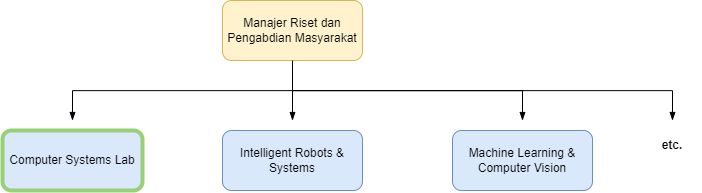
\includegraphics[width=1\textwidth]
	{assets/pics/pacil-org.png}
	\caption{Struktur Organisasi Pusat Penelitian Fakultas Ilmu Komputer UI}
	\label{fig:pacil-org}
\end{figure}

Dijelaskan pada \pic~\ref{fig:pacil-org} bahwa Computer Systems Laboratory (CSL) berada di bawah supervisi Manajer Riset dan Pengabdian Masyarakat, bersama dengan beberapa pusat penelitian lainnya, seperti Intelligent Robots \& Systems (IRoS) dan Machine Learning \& Computer Vision (MLCV). Struktur organisasi di CSL sendiri bersifat flat, di mana setiap penelitian dilakukan secara independen oleh masing-masing tim atau individu. Namun ada dosen peneliti yang bertanggung jawab memantau seluruh proyek untuk memastikan semua penelitian berjalan sesuai standar akademik.

Pelaksana kerja praktik ditempatkan dalam tim yang mengerjakan penelitian manajemen cluster Kafka, yang berfokus pada optimasi performa sistem distribusi data \textit{real-time}. Sebagai \textit{Research Assistant}, pelaksana terlibat langsung dalam berbagai tahap eksperimen, mulai dari penyiapan infrastruktur hingga analisis hasil.

\clearchapter
\chapter{\babDua}
\label{bab:2}
Pada bab ini dijlaskan secara rinci mengenai detil pekerjaan yang dilakukan selama program kerja praktik berlangsung. Latar belakang pekerjaan hingga hasil pekerjaan dijelaskan pada bab ini.

\section{Latar Belakang Pekerjaan}

Pelaksana kerja praktik terlibat dalam penelitian terkait manajemen klaster Kafka di Computer Systems Laboratory (CSL) Fakultas Ilmu Komputer Universitas Indonesia. Penelitian ini berfokus pada optimalisasi partisi topik untuk meningkatkan performa \textit{real-time distributed systems} berbasis Kafka. Proyek ini merupakan bagian dari penelitian bertajuk \textit{Efficient Topic Partitioning of Apache Kafka for High-Reliability Real-Time Data Streaming Applications}. Tugas pelaksana kerja praktik adalah menjalankan eksperimen yang bertujuan untuk menguji algoritma BroMax dan BroMin, yang digunakan untuk menentukan jumlah partisi optimal.

\section{Deskripsi Pekerjaan}

Pelaksana kerja praktik bertanggung jawab atas konfigurasi dan pengelolaan eksperimen \textit{end-to-end}. Proses dimulai dengan penyiapan VM di Google Cloud Platform (GCP) dan infrastruktur Universitas Indonesia (DGX dan BMKGCS), yang digunakan untuk menjalankan simulasi klaster Kafka. Tugas utama meliputi instalasi dependencies, pengaturan Kafka broker, serta analisis hasil eksperimen untuk mengukur performa sistem, khususnya \textit{throughput} dan latensi, saat algoritma BroMax dan BroMin diterapkan.

Pekerjaan dilakukan secara \textit{hybrid} dari pukul 08.00 a.m. WIB hingga pukul 12.00 p.m. WIB, dengan kehadiran di lab hanya pada hari Jumat, sedangkan hari-hari lainnya bekerja secara \textit{remote}. Hasil eksperimen dianalisis dan dilaporkan kepada dosen peneliti untuk evaluasi lebih lanjut.

\section{Tinjauan Pustaka}

Penelitian yang dilakukan selama kerja praktik ini melibatkan sejumlah konsep penting dalam pengelolaan \textit{real-time distributed systems} dengan menggunakan Apache Kafka dan teknologi pendukung lainnya. Konsep-konsep ini menjadi fondasi utama dalam penelitian dan pengembangan yang dilakukan.

\subsection{Apache Kafka}

Apache Kafka adalah platform \textit{open-source} yang dirancang untuk menangani \textit{data streaming} secara \textit{real-time} dengan \textit{throughput} tinggi dan latensi rendah. Data dibagi menjadi topik-topik yang dipartisi, sehingga memungkinkan pemrosesan paralel yang lebih efisien di seluruh klaster \citep{elsevier:kafka}. Partisi pada topik Kafka sangat penting karena memungkinkan distribusi beban kerja yang merata antar broker, sehingga meningkatkan kemampuan sistem untuk menangani data dalam jumlah besar tanpa menimbulkan \textit{bottleneck} \citep{elsevier:kafka}. Selain itu, dengan optimalisasi jumlah partisi yang tepat, \textit{throughput} sistem dapat dimaksimalkan, sehingga menjaga kinerja tinggi meskipun volume data yang diproses sangat besar \citep{elsevier:kafka}.

\subsection{Docker Containerization}

Docker Containerization adalah teknologi yang memungkinkan aplikasi dijalankan dalam \textit{container} yang terisolasi, sehingga dapat memisahkan lingkungan eksekusi aplikasi dari sistem \textit{host}. Docker memungkinkan konsistensi lingkungan, meminimalkan konflik konfigurasi, serta meningkatkan portabilitas sistem \citep{its:docker}. Dengan Docker, seluruh proses \textit{deployment} Kafka menjadi lebih efisien karena setiap \textit{node} dalam klaster dapat dijalankan dengan konfigurasi yang seragam, sehingga mengurangi kesalahan operasional \citep{its:docker}.

\subsection{Apache Zookeeper}

Apache Zookeeper adalah layanan koordinasi terpusat yang digunakan untuk mengelola \textit{metadata} dan menjaga konsistensi di dalam klaster Kafka. Zookeeper bertugas mengatur eleksi pemimpin partisi, menyinkronkan data antar broker, serta memastikan bahwa setiap perubahan dalam klaster Kafka ditangani dengan cepat dan efisien \citep{comp:zookeeper}. Dalam konteks Kafka, Zookeeper memainkan peran penting dalam memastikan bahwa sistem tetap \textit{fault-tolerant}. Jika terjadi kegagalan pada salah satu broker, Zookeeper secara otomatis memilih broker lain untuk menjadi pemimpin, sehingga menjaga kestabilan sistem \citep{comp:zookeeper}. Zookeeper juga menyimpan informasi konfigurasi mengenai topik dan partisi Kafka, dan memastikan bahwa produser dan konsumen dapat berinteraksi dengan sistem secara konsisten \citep{comp:zookeeper}.

\subsection{Distributed System}

Distributed System adalah sistem yang terdiri dari beberapa \textit{node} yang terhubung dan bekerja bersama untuk mencapai tujuan tertentu. Dalam konteks Kafka, sistem terdistribusi ini memastikan bahwa data dapat diolah secara paralel dan skalabel di berbagai broker yang tersebar dalam klaster. Keunggulan dari sistem terdistribusi seperti Kafka adalah kemampuannya untuk tetap berfungsi meskipun terjadi kegagalan pada satu atau beberapa \textit{node} dalam klaster \citep{ieee:distributed}. Dalam sistem terdistribusi Kafka, partisi topik didistribusikan ke berbagai broker, sehingga meningkatkan ketersediaan data dan mempercepat proses pengiriman data dari produser ke konsumen \citep{ieee:distributed}. Sistem ini juga memungkinkan replikasi data secara otomatis, di mana salinan data disimpan di beberapa broker untuk meningkatkan keandalan dan redundansi sistem \citep{ieee:distributed}.

\section{Metodologi Pekerjaan}

Metodologi eksperimental kuantitatif dalam proyek ini melibatkan pengumpulan dan analisis data numerik secara end-to-end untuk mengukur performa Apache Kafka pada berbagai konfigurasi sistem. Tahapan pekerjaan yang dilaksanakan secara bertahap sesuai dengan proses yang dirancang, mulai dari pengaturan infrastruktur hingga analisis hasil eksperimen. Berikut adalah tahapan metodologi pekerjaan yang dilakukan selama kerja praktik:

\begin{enumerate}

	\item \textbf{Pengaturan VM}. Langkah awal dalam kerja praktik ini adalah menyiapkan VM (Virtual Machine) di Google Cloud Platform (GCP). VM tersebut dikonfigurasi menggunakan SSH dengan akses \textit{root}. Setelah VM disiapkan, seluruh dependensi yang diperlukan untuk menjalankan eksperimen Kafka diinstal. Konfigurasi ini memastikan bahwa VM siap untuk menjalankan berbagai eksperimen Kafka, di mana satu VM bertindak sebagai Kafka \textit{client}, dan VM lainnya berperan sebagai Kafka \textit{cluster}. Seluruh pengaturan ini bertujuan untuk mendukung kelancaran eksperimen yang dilakukan.

	\item \textbf{Eksekusi Eksperimen End-To-End}.
	
	\begin{figure}
		\centering
		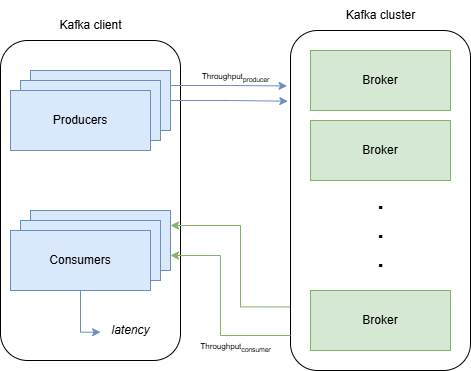
\includegraphics[width=1\textwidth]
		{assets/pics/end-to-end-experiment.png}
		\caption{Eksekusi Eksperimen \textit{End-To-End}}
		\label{fig:end-to-end-experiment}
	\end{figure}
	
	Setelah pengaturan infrastruktur selesai, eksperimen dilakukan dengan fokus pada simulasi \textit{end-to-end} yang bertujuan untuk memantau algoritma BroMax dan BroMin dalam menentukan jumlah partisi dan broker pada sistem Apache Kafka. Terlihat pada \pic~\ref{fig:end-to-end-experiment} bahwa eksperimen ini melibatkan pengaturan dua VM dengan fungsi yang berbeda: satu VM bertindak sebagai Kafka client yang mengirimkan dan menerima data, sedangkan VM lainnya bertindak sebagai Kafka cluster berisi broker yang mengelola partisi. Eksperimen ini penting untuk memahami perilaku \textit{throughput} dan latensi sistem secara keseluruhan dalam kondisi yang mendekati \textit{real-time streaming}. Hasil dari eksperimen ini memberikan wawasan tentang cara kerja algoritma BroMax dan BroMin dalam optimasi partisi.

	\item \textbf{Pemantauan Sumber Daya}. Selama eksperimen berlangsung, pemantauan sumber daya dilakukan secara berkala untuk memantau penggunaan CPU, RAM, dan \textit{disk space} pada VM. Hal ini penting untuk memastikan bahwa eksperimen berjalan dengan efisien tanpa ada \textit{bottleneck} dalam pemanfaatan sumber daya. Data yang dihasilkan dari pemantauan sumber daya ini juga menjadi acuan dalam mengevaluasi performa algoritma BroMax dan BroMin.

	\item \textbf{Eksperimen Infrastruktur UI}. Setelah eksperimen di GCP berhasil dilaksanakan, eksperimen serupa diulang pada infrastruktur UI menggunakan mesin DGX dan BMKGCS tanpa akses \textit{root}. Eksperimen ini dilakukan untuk memastikan bahwa hasil eksperimen dapat direplikasi di lingkungan yang berbeda dengan kapasitas sumber daya yang lebih besar.

	\item \textbf{Implementasi Containerization dengan Docker}. Dalam eksperimen ini, Docker digunakan untuk membangun dan mengelola \textit{container} yang berisi aplikasi Apache Kafka. Pelaksana kerja praktik mempelajari cara kerja Docker, mulai dari membangun \textit{image} hingga pengaturan komunikasi antar \textit{container}. Dengan \textit{containerization}, eksperimen dapat dijalankan pada \textit{host} tanpa akses \textit{root} sekalipun. Eksperimen ini juga mengeksplorasi penggunaan teknologi Docker-in-Docker (DinD) ketika membuat Kafka \textit{scluster container} yang di dalamnya berisi beberapa \textit{sbroker containers}.

	\item \textbf{Analisis Data dan Pelaporan}. Setelah seluruh eksperimen selesai dijalankan, data hasil eksperimen dianalisis untuk membuat plot yang menggambarkan performa \textit{throughput} dan latensi sistem. Plot ini kemudian digunakan untuk mendeskripsikan perilaku algoritma BroMax dan BroMin dalam kondisi eksperimen yang telah dilakukan. Hasil analisis ini kemudian disajikan dalam laporan kepada dosen peneliti, serta didiskusikan dengan para peneliti lainnya untuk mendapatkan umpan balik dan evaluasi lebih lanjut mengenai hasil eksperimen.

\end{enumerate}

\section{Teknologi}

Selama pengerjaan proyek pada kerja praktik, beberapa teknologi utama digunakan untuk mendukung penelitian. Berikut adalah teknologi-teknologi tersebut:

\begin{itemize}

	\item \textbf{Apache Kafka}, Sebuah platform yang digunakan untuk memproses data secara paralel dan \textit{real-time} melalui topik yang dipartisi. Kafka memungkinkan penanganan volume data yang sangat besar dengan \textit{throughput} tinggi dan latensi rendah, serta mendukung replikasi data untuk menjaga keandalan sistem.

	\item \textbf{Docker}, Merupakan platform \textit{containerization} yang memungkinkan pengembang menjalankan aplikasi dalam lingkungan terisolasi yang disebut container. Docker digunakan untuk menyederhanakan \textit{deployment} sistem Apache Kafka dan komponen lainnya selama eksperimen. Docker memastikan lingkungan yang seragam dan memudahkan migrasi antar infrastruktur.

	\item \textbf{Linux}, Sistem operasi \textit{open-source} yang digunakan dalam menjalankan berbagai komponen pada infrastruktur server. Linux menawarkan stabilitas dan kontrol penuh terhadap manajemen sumber daya, yang sangat penting untuk menjalankan aplikasi terdistribusi seperti Kafka dan Docker.

	\item \textbf{Bash}, Bash adalah bahasa skrip yang digunakan untuk mengotomatisasi berbagai tugas di lingkungan Linux. Dalam proyek ini, Bash digunakan untuk menjalankan skrip yang mengelola proses \textit{deployment}, \textit{system monitoring}, dan pemeliharaan sumber daya.

	\item \textbf{Python}, Sebuah bahasa pemrograman yang digunakan untuk menulis skrip otomasi dan pengolahan data. Python sangat fleksibel dan mendukung banyak \textit{library} untuk analisis data, pemantauan sistem, dan integrasi dengan platform lain seperti Kafka.

	\item \textbf{Google Cloud Platform (GCP)}, GCP adalah platform komputasi awan yang menyediakan infrastruktur untuk menjalankan VM yang mendukung eksperimen Kafka. GCP digunakan untuk skala dan fleksibilitas, memungkinkan pengembang menguji aplikasi di lingkungan cloud yang efisien.

	\item \textbf{WhatsApp}, Sebagai aplikasi perpesanan, WhatsApp digunakan dalam konteks komunikasi informal antara tim dan dosen peneliti selama proyek.

\end{itemize}

\section{Hasil Pekerjaan}

Selama periode kerja praktik, pelaksana terlibat dalam tugas-tugas yang menuntut analisis mendalam terkait {real-time data streaming} menggunakan Apache Kafka. Pada bagian ini dijelaskan tugas apa saja yang sudah diselesaikan pada periode kerja praktik berlangsung.

\subsection{Framework Berbasis Containerization dengan Pendekatan Docker-in-Docker (DinD)}

Pelaksana kerja praktik mengusulkan ide kepada dosen peneliti untuk mengembangkan \textit{framework} berbasis \textit{containerization} dengan pendekatan Docker-in-Docker (DinD). \textit{Framework} ini dirancang agar dapat mengotomatisasi seluruh proses \textit{setup}, termasuk pembuatan Kafka \textit{scluster container} yang di dalamnya berisi beberapa \textit{sbroker containers}, tanpa perlu akses \textit{root} pada \textit{host}, sehingga pengguna hanya perlu menjalankan sedikit skrip tanpa perlu mengulang pengaturan secara manual. Dengan adanya \textit{framework} ini, pelaksana kerja praktik dapat langsung fokus pada analisis eksperimen tanpa harus khawatir tentang masalah teknis terkait lingkungan yang berulang kali harus disesuaikan. \textit{Framework} ini dapat diakses oleh siapa saja melalui \textcolor{blue}{\href{https://github.com/bryan-ilman-on-github/kafka-part-exp}{https://github.com/bryan-ilman-on-github/kafka-part-exp}}.

\subsection{Analisis Eksperimen End-To-End}

\begin{figure}
	\centering
	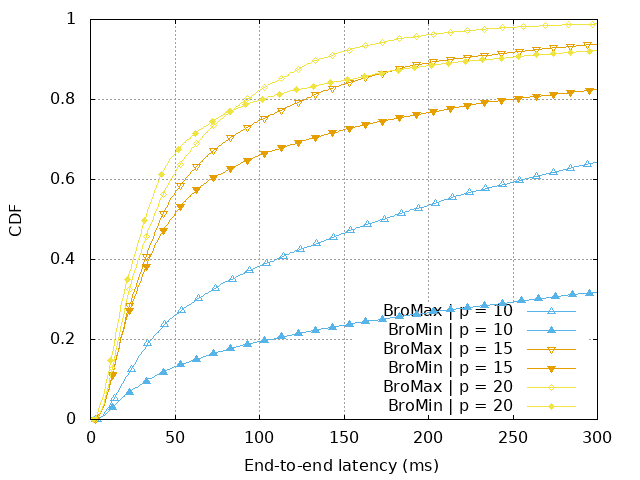
\includegraphics[width=1\textwidth]
	{assets/pics/latency-cdf.png}
	\caption{Analisis Eksperimen \textit{End-To-End}}
	\label{fig:latency-cdf}
\end{figure}

Salah satu temuan utama dari eksperimen ini adalah bahwa metode penentuan jumlah partisi sangat memengaruhi \textit{throughput} dan latensi. \pic~\ref{fig:latency-cdf} menampilkan CDF, yaitu garis kurva yang menunjukkan persentase kumulatif latency pada \textit{millisecond} tertentu. Garis yang lebih tinggi di awal menunjukkan lebih banyak latency rendah, yang berarti performa lebih baik. Terlihat pada \pic~\ref{fig:latency-cdf} bahwa algoritma BroMax, yang aktif memaksimalkan penggunaan semua sumber daya yang tersedia untuk mendistribusikan beban kerja, berhasil mempertahankan latensi yang rendah sehingga menghasilkan \textit{throughput} yang relatif lebih tinggi. Sebaliknya, algoritma BroMin, yang lebih konservatif dalam penggunaan sumber daya, cenderung memiliki latensi yang sedikit lebih tinggi, sehingga \textit{throughput}-nya relatif lebih rendah.

Selain itu, terlihat pula pada \pic~\ref{fig:latency-cdf} bahwa jumlah produsen yang lebih banyak justru mengurangi latensi secara keseluruhan, berlawanan dengan intuisi awal yang menganggap bahwa lebih banyak produsen akan meningkatkan beban klaster dan menyebabkan latensi lebih tinggi. Setelah diskusi dengan tim, didapat penjelasan untuk temuan ini bahwa tingginya \textit{overhead} pada klaster dengan sedikit produsen tidak ideal untuk beban kerja yang sebenarnya. Sebaliknya, pada klaster dengan lebih banyak produsen, \textit{overhead} menjadi tidak signifikan dibandingkan dengan beban kerja yang ada, sehingga performanya lebih stabil. Hasil eksperimen ini memberikan wawasan yang lebih mendalam tentang pengoptimalan konfigurasi klaster Kafka.

\section{Aspek Non Teknis}

Dalam pelaksanaan kerja praktik, terdapat berbagai pembelajaran non-teknis yang turut berperan penting dalam mendukung keberhasilan tugas. Aspek-aspek seperti komunikasi dan kerja sama tim menjadi bagian integral dari keseluruhan pengalaman kerja praktik.

\subsection{Komunikasi}

\begin{figure}
	\centering
	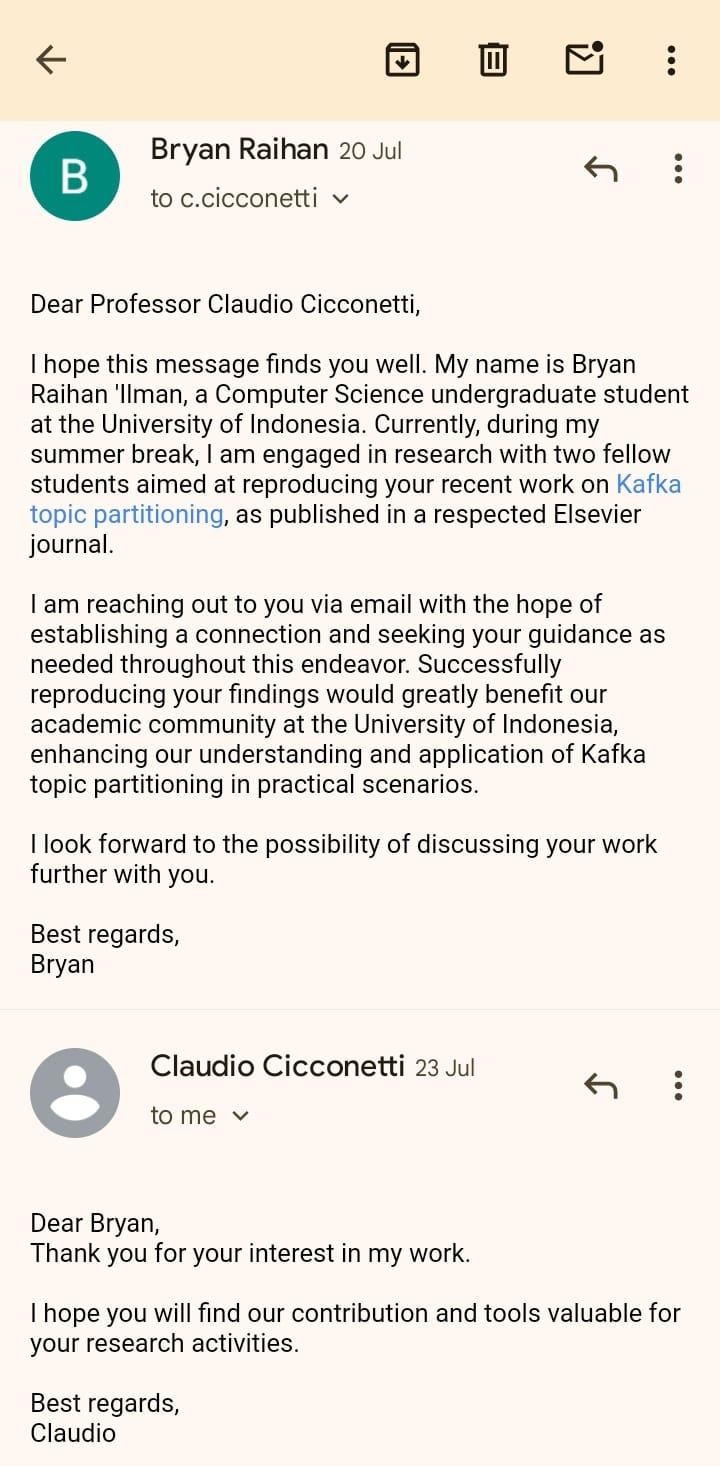
\includegraphics[width=0.5\textwidth]
	{assets/pics/first-email.png}
	\caption{Email Pertama dari Profesor Claudio}
	\label{fig:first-email}
\end{figure}

Selama kerja praktik, komunikasi memainkan peranan yang sangat penting dalam memastikan kelancaran proyek dan kesesuaian hasil dengan tujuan yang ditetapkan. Salah satu contoh penting dalam hal ini adalah komunikasi yang dilakukan melalui email dengan Profesor Claudio Cicconetti dari Università di Pisa, penulis penelitian yang eksperimennya sedang pelaksana kerja praktik coba untuk replikasi. Terlihat pada \pic~\ref{fig:first-email} bahwa pelaksana kerja praktik pertama kali menginformasikan kepada Profesor Cicconetti bahwa eksperimennya sedang direproduksi. Setelah itu, email-email selanjutnya berfokus pada klarifikasi mengenai beberapa aspek teknis dari penelitiannya, dan beliau dengan ramah memberikan tanggapan serta penjelasan yang sangat membantu. Hal ini menekankan pentingnya komunikasi yang efektif dalam lingkungan akademik dan profesional, terutama saat bekerja dengan pihak eksternal yang memiliki keahlian khusus dalam bidang tertentu.

\subsection{Kerja Sama Tim}

Kerja sama tim merupakan aspek lain yang sangat penting dalam pelaksanaan proyek selama kerja praktik. Dalam mengerjakan proyek, tidak ada tugas yang dilakukan sepenuhnya secara mandiri. Setiap anggota tim memiliki peran spesifik yang saling berhubungan, dan keberhasilan satu bagian proyek sering kali tergantung pada penyelesaian bagian lain yang dikerjakan oleh anggota tim lain.

\section{Analisis Pelaksanaan Kerja Praktik}

Pada bagian ini dijelaskan analisis menyeluruh mengenai pelaksanaan kerja praktik. Penjelasan dimulai dengan mengkaji kesesuaian pelaksanaan kerja praktik terhadap kerangka acuan kerja praktik yang telah disusun. Selain itu, kendala-kendala yang muncul selama kerja praktik berlangsung juga akan diuraikan, beserta solusi yang diterapkan untuk mengatasi hambatan tersebut.

\newpage

\subsection{Ulasan kesesuaian dan perbedaan dengan KAKP}

\begin{longtable}{|p{2.6cm}|p{8cm}|c|}
	\caption{Perbandingan Rencana dan Realisasi Kerja Praktik}
	\label{tab:realisasi-kerja} \\
	\hline
    \textbf{Waktu} & \textbf{Rencana Kerja} & \textbf{Realisasi Kerja} \\
    \hline
    Minggu 1\newline
	(3 Juni 2024 -- 7 Juni 2024) &
	\textbf{Meninjau jurnal dari Elsevier dan mencari penelitian terbaru mengenai Apache Kafka yang dapat diterapkan kembali di CSL.}\newline
	-- Menganalisis metodologi dan hasil dari paper berjudul "Efficient topic partitioning of Apache Kafka for high-reliability real-time data streaming applications".\vspace{0.5cm}\newline
	\textbf{Bergabung dengan Komunitas FogVerse.}\newline
	-- Bergabung dengan komunitas FogVerse di WhatsApp dan Discord.\vspace{0.5cm} &
	Sesuai dengan KAKP \\
    \hline
    Minggu 2\newline
	(10 Juni 2024 -- 14 Juni 2024) &
	\textbf{Merumuskan langkah-langkah untuk menerapkan kembali isi paper.}\newline
	-- Membaca dan memahami paper yang akan	diterapkan kembali.\newline
	-- Merancang langkah-langkah secara detail.\vspace{0.5cm}\newline
	\textbf{Mengikuti perkembangan proyek flagship CSL, yaitu FogVerse.}\newline
	-- Mempelajari kode FogVerse dari GitHub.\newline
	-- Mengunduh kode FogVerse.\vspace{0.5cm} &
	Sesuai dengan KAKP \\
	\hline
    Minggu 3\newline
	(17 Juni 2024 -- 21 Juni 2024) &
	\textbf{Mengkaji kode Kafka Topic Partitioning yang ada	di paper.}\newline
	-- Memeriksa kode untuk eksperimen, memastikan semua baris kode telah terkumpul.\newline
	-- Merumuskan seluruh dependensi yang diperlukan.\vspace{0.5cm} &
	Sesuai dengan KAKP \\
	\hline
    Minggu 4\newline
	(24 Juni 2024 -- 28 Juni 2024) &
	\textbf{Mengatur pertemuan dan menyiapkan presentasi awal.}\newline
	-- Mengatur pertemuan dengan Brandon dan Ikram, yang merupakan penerus penelitian flagship tentang Kafka di CSL.\newline
	-- Menyiapkan file serta pertanyaan untuk presentasi awal kepada Bapak Hilman tentang progres.\vspace{0.5cm} &
	Sesuai dengan KAKP \\
	\hline
    Minggu 5\newline
	(1 Juli 2024 -- 5 Juli 2024) &
	\textbf{Merencanakan dan mengatur spesifikasi VM di	GCP.}\newline
	-- Mengatur dan menghubungkan dua VM tempat	eksperimen di GCP. kedua VM akan digunakan untuk Kafka Cluster dan Kafka Clients.\newline
	-- Melakukan eksperimen kalibrasi (bukan eksperimen	utama).\vspace{0.5cm} &
	Sesuai dengan KAKP \\
	\hline
    Minggu 6\newline
	(8 Juli 2024 -- 12 Juli 2024) &
	\textbf{Membagi tugas eksperimen.}\newline
	-- Membagi tugas eksperimen dengan Rifqi dan Anin, yang merupakan rekan dalam menerapkan ulang paper.\newline
	-- Memodifikasi spesifikasi VM untuk mengatasi masalah selama eksperimen.\vspace{0.5cm} &
	Sesuai dengan KAKP \\
	\hline
    Minggu 7\newline
	(15 Juli 2024 -- 19 Juli 2024) &
	\textbf{Menjalankan eksperimen.}\newline
	-- Menjalankan eksperimen utama yang merupakan inti dari penerapan ulang paper.\newline
	-- Memeriksa performa VM.\newline
	-- Menyampaikan kebutuhan sumber daya kepada Bapak Hilman jika diperlukan.\vspace{0.5cm} &
	Sesuai dengan KAKP \\
	\hline
    Minggu 8\newline
	(22 Juli 2024 -- 26 Juli 2024) &
	\textbf{Membuat plot dan menganalisis hasil eksperimen.}\newline
	-- Membuat plot dari hasil eksperimen.\newline
	-- Menganalisis hasil eksperimen.\newline
	-- Berdiskusi dengan tim tentang kemajuan eksperimen dan hasil yang diperoleh.\vspace{0.5cm} &
	Sesuai dengan KAKP \\
	\hline
    Minggu 9\newline
	(29 Juli 2024 -- 2 Agustus 2024) &
	\textbf{Melakukan ulang eksperimen pada infrastruktur UI.}\newline
	-- Mengakses mesin DGX dan mesin BMKGCS milik UI, yang memiliki sumber daya jauh lebih besar dibandingkan VM murah di GCP, untuk mendekati kondisi penelitian asli.\newline
	-- Melakukan eksperimen hingga jalan.\vspace{0.5cm} &
	Sesuai dengan KAKP \\
	\hline
    Minggu 10\newline
	(5 Agustus 2024 -- 9 Agustus 2024) &
	\textbf{Melakukan ulang eksperimen dengan Setup	Docker-in-Docker pada infrastruktur UI.}\newline
	-- Melakukan ulang eksperimen pada infrastruktur UI	dengan batasan VM seperti yang dijelaskan dalam paper, agar lebih mirip dengan penelitian asli. Untuk ini, diperlukan pengaturan Docker-in-Docker agar container yang berisi Kafka cluster dan Kafka clients dapat dikonfigurasi tanpa perlu root access pada hostnya.\vspace{0.5cm}\newline
	\textbf{Membuat plot dan menganalisis hasil eksperimen.}\newline
	-- Membuat plot dari hasil eksperimen.\newline
	-- Menganalisis hasil eksperimen.\newline
	-- Berdiskusi dengan tim tentang kemajuan eksperimen dan hasil yang diperoleh.\vspace{0.5cm} &
	Sesuai dengan KAKP \\
	\hline
    Minggu 11\newline
	(12 Agustus 2024 -- 16 Agustus 2024) &
	\textbf{Mengatur pertemuan dengan peneliti asli.}\newline
	-- Menghubungi Profesor Claudio Cicconetti melalui email untuk merencanakan pertemuan online.\newline
	-- Mengadakan pertemuan dengan Claudio Cicconetti untuk klarifikasi hal-hal yang masih diragukan dan meminta evaluasinya.\vspace{0.5cm} &
	Sesuai dengan KAKP \\
	\hline
    Minggu 12\newline
	(19 Agustus 2024 -- 23 Agustus 2024) &
	\textbf{Melakukan presentasi akhir.}\newline
	-- Menyampaikan laporan hasil kegiatan kepada Bapak Hilman.\vspace{0.5cm}\newline
	\textbf{Menyusun laporan akhir kerja praktik untuk keperluan fakultas.}\vspace{0.5cm} &
	Sesuai dengan KAKP \\
    \hline
\end{longtable}

Seperti yang dapat dilihat pada \tab~\ref{tab:realisasi-kerja}, secara keseluruhan, pelaksanaan kerja praktik telah berjalan sesuai dengan yang tercantum dalam Kerangka Acuan Kerja Praktik (KAKP). Semua target yang telah ditetapkan terlaksana dengan baik, dan tidak ada permintaan yang melebihi apa yang telah diuraikan dalam KAKP.

\subsection{Ulasan tentang kendala dan cara menanganinya}

Selama kerja praktik, beberapa kendala teknis muncul, berkaitan langsung dengan pekerjaan yang dilakukan. Setiap kendala yang ada diatasi dengan solusi yang sesuai untuk memastikan eksperimen tetap berjalan lancar.

\subsubsection{Tidak Memiliki Akses Root pada Infrastruktur UI}

Salah satu kendala utama yang muncul selama kerja praktik adalah keterbatasan akses \textit{root} pada infrastruktur Universitas Indonesia (UI). Akses \textit{root} sangat penting dalam eksperimen, terutama untuk mengunduh \textit{library} atau melakukan konfigurasi yang lebih mendalam pada sistem. Tanpa akses ini, beberapa langkah teknis yang memerlukan izin tingkat sistem tidak dapat dilakukan secara langsung, sehingga menghambat kelancaran eksperimen. Kondisi ini menuntut solusi yang inovatif untuk mengatasi batasan tersebut.

Untuk mengatasi kendala ini, diterapkan solusi \textit{containerization} dengan dibuatnya Kafka \textit{client container} dan Kafka \textit{cluster container}. Lebih spesifiknya, pendekatan yang diambil adalah Docker-in-Docker (DinD) karena di dalam Kafka \textit{cluster container}, terdapat banyak \textit{broker containers} yang berjalan secara paralel. Pendekatan ini memungkinkan pengunduhan dan instalasi \textit{library} secara independen di dalam lingkungan yang terisolasi tanpa memerlukan akses \textit{root} langsung pada mesin \textit{host}.

\subsubsection{Dokumentasi dari Peneliti Asli Kurang Lengkap atau Usang}

Kendala lain yang dihadapi adalah dokumentasi penelitian asli yang tidak lengkap atau sudah usang. Dokumentasi dari penelitian yang direplikasi sering kali tidak menyertakan penjelasan yang detail mengenai setiap langkah yang dilakukan, atau sudah tidak relevan dengan perkembangan teknologi terbaru. Hal ini menimbulkan tantangan dalam mengikuti alur eksperimen dan mencapai hasil yang sama seperti yang dicapai oleh peneliti sebelumnya.

Untuk mengatasi masalah ini, dilakukan improvisasi terhadap beberapa langkah eksperimen. Pelaksana kerja praktik memanfaatkan referensi tambahan dan hasil riset terbaru untuk menyesuaikan langkah-langkah yang tidak dijelaskan dalam dokumentasi. Selain itu, pelaksana kerja praktik juga mengandalkan hasil komunikasi dengan Profesor Claudio Cicconetti untuk memperoleh klarifikasi lebih lanjut mengenai metode yang diterapkan.

\subsubsection{Penggunaan Resource yang Besar}

Salah satu tantangan terbesar yang pelaksana kerja praktik hadapi selama kerja praktik adalah kebutuhan sumber daya komputasi yang sangat tinggi, terutama saat menjalankan eksperimen di Google Cloud Platform (GCP). Awalnya, konfigurasi awal VM yang dibuat tidak memiliki cukup kapasitas untuk menangani eksperimen berat yang melibatkan proses \textit{real-time data streaming} menggunakan Apache Kafka. Keterbatasan ini menyebabkan VM sering kali kehabisan memori atau mengalami penurunan performa, yang berdampak pada tidak optimalnya hasil eksperimen.

Untuk mengatasi masalah ini, dilakukan beberapa iterasi dalam penyesuaian alokasi sumber daya pada VM di GCP. Setelah beberapa percobaan dan pemantauan terhadap penggunaan CPU dan RAM, ditemukan bahwa eksperimen ini memerlukan alokasi sebesar 128 GB RAM dan 64 core CPU agar dapat berjalan dengan lancar tanpa hambatan. Dengan peningkatan sumber daya ini, eksperimen berhasil berjalan dengan performa optimal.

\subsection{Penilaian Individu Terhadap Tempat Kerja Praktik}

CSL merupakan lingkungan kerja yang dinamis dan menyenangkan. Banyak inovasi baru yang dihasilkan oleh mahasiswa yang sedang mengerjakan tesis atau skripsi, sehingga menciptakan atmosfer yang kreatif dan kolaboratif. Selain itu, CSL memberikan kesempatan untuk menerapkan teori-teori yang didapat dari perkuliahan ke dalam praktik nyata, sehingga menjadi tempat yang ideal untuk mengembangkan keterampilan teknis.

\subsection{Relevansi dengan Perkuliahan}

Selama kerja praktik, beberapa tugas yang diberikan memiliki relevansi langsung dengan pembelajaran yang didapatkan dari beberapa mata kuliah di Fakultas Ilmu Komputer UI. Berikut adalah mata kuliah yang relevan:

\subsubsection{Sistem Operasi}
Mata kuliah Sistem Operasi memberikan pemahaman tentang penggunaan GNU/Linux, \textit{rscripting bash}, serta manajemen proses dan memori. Pengetahuan ini sangat berguna selama kerja praktik, di mana \textit{rbash scripting} digunakan untuk mengotomatisasi tugas-tugas tertentu dan mengonfigurasi virtual machine.

\subsubsection{Jaringan Komputer}
Mata kuliah ini memberikan dasar yang kuat tentang prinsip-prinsip jaringan, mulai dari lapisan aplikasi hingga lapisan fisik, serta aspek keamanan jaringan. Selama kerja praktik, pemahaman ini diterapkan untuk memastikan aliran data berjalan lancar, mengatur koneksi SSH, dan mengelola setup VM di platform seperti GCP dan infrastruktur UI, sehingga komunikasi jaringan dan pengalokasian sumber daya berjalan dengan optimal.

\subsubsection{Pemrograman Lanjut}
Pada mata kuliah Pemrograman Lanjut, dipelajari konsep manajemen pesan dengan RabbitMQ. Di tempat kerja praktik, konsep ini diterapkan menggunakan Apache Kafka, sebuah platform yang lebih sesuai untuk kebutuhan \textit{rreal-time data streaming} yang kompleks.

\clearchapter
%-----------------------------------------------------------------------------%
\chapter{\babTiga}
\label{bab:3}
%-----------------------------------------------------------------------------%
Bab ini menjelaskan tentang hal-hal \f{advanced} dalam \latex.
Hal ini mencakup bagaimana cara menulis persamaan matematis di \latex, menambahkan daftar isi, catatan, PDF, menambahkan kode, bahkan menambahkan perintah baru.

\noindent\todo{
	Sejatinya bab ini digunakan untuk membahas inti dari penelitian Anda.
	Sesuaikan saja dengan kebutuhkan Anda: misalkan bab tiga Anda adalah penjelasan terkait desain sistem.
}


%-----------------------------------------------------------------------------%
\section{Membuat Persamaan Matematis}
\label{sec:mathEqu}
%-----------------------------------------------------------------------------%
Di \latex, kita dapat membuat persamaan matematis baik yang terdiri dari satu persamaan maupun lebih dari satu persamaan.
Anda bisa mencoba mengikuti dan memahami contoh kode yang ada di \f{template} ini untuk kebutuhan tugas akhir Anda.
Menggunakan \latex~juga perlu latihan dan lihai memahami dokumentasi.

%-----------------------------------------------------------------------------%
\subsection{Satu Persamaan}
\label{sec:oneEqu}
%-----------------------------------------------------------------------------%

\noindent \begin{align}\label{equ:garis}
	\cfrac{y - y_{1}}{y_{2} - y_{1}} =
	\cfrac{x - x_{1}}{x_{2} - x_{1}}
\end{align}

\equ~\ref{equ:garis} diatas adalah persamaan garis.
\equ~\ref{equ:garis} dan \ref{equ:bola} sama-sama dibuat dengan perintah \code{\bslash{}align}.
Perintah ini juga dapat digunakan untuk menulis lebih dari satu persamaan.

\noindent \begin{align}\label{equ:bola}
	\underbrace{|\overline{ab}|}_{\text{pada bola $|\overline{ab}| = r$}}
	= \sqrt[2]{(x_{b} - x_{a})^{2} + (y_{b} - y_{a})^{2} +
		\vert\vert(z_{b} - z_{a})^{2}}
\end{align}

%-----------------------------------------------------------------------------%
\subsection{Lebih dari Satu Persamaan}
\label{sec:multiEqu}
%-----------------------------------------------------------------------------%
\noindent \begin{align}\label{equ:matriks}
	|\overline{a} * \overline{b}| &= |\overline{a}| |\overline{b}| \sin\theta
	\\[0.2cm]
	\overline{a} * \overline{b} &=
	\begin{array}{| c c c |}
		\hat{i} & x_{1} & x_{2} \\
		\hat{j} & y_{1} & y_{2} \\
		\hat{k} & z_{1} & z_{2} \\
	\end{array} \nonumber \\[0.2cm]
	&= \hat{i} \,
	\begin{array}{ | c c | }
		y_{1} & y_{2} \\
		z_{1} & z_{2} \\
	\end{array}
	+ \hat{j} \,
	\begin{array}{ | c c | }
		z_{1} & z_{2} \\
		x_{1} & x_{2} \\
	\end{array}
	+ \hat{k} \,
	\begin{array}{ | c c | }
		x_{1} & x_{2} \\
		y_{1} & y_{2} \\
	\end{array}
	\nonumber
\end{align}

Pada \equ~\ref{equ:matriks} dapat dilihat beberapa baris menjadi satu bagian
dari \equ~\ref{equ:matriks}.
Sedangkan dibawah ini dapat dilihat bahwa dengan cara yang sama, \equ~
\ref{equ:gabungan1}, \ref{equ:gabungan2}, dan \ref{equ:gabungan3} memiliki nomor
persamaannya masing-masing.

\noindent \begin{align}\label{equ:gabungan1}
	\int_{a}^{b} f(x)\, dx + \int_{b}^{c} f(x) \, dx = \int_{a}^{c} f(x) \, dx
	\\\label{equ:gabungan2}
	\lim_{x \to \infty} \frac{f(x)}{g(x)} = 0 \hspace{1cm}
	\text{jika pangkat $f(x)$ $<$ pangkat $g(x)$} \\\label{equ:gabungan3}
	a^{m^{a \, ^{n}\log b }} = b^{\frac{m}{n}}
\end{align}



%-----------------------------------------------------------------------------%
\section{Mengubah Tampilan Teks}
\label{sec:textFormatting}
%-----------------------------------------------------------------------------%
Beberapa perintah yang dapat digunakan untuk mengubah tampilan adalah:
\begin{itemize}
	\item \bslash{}f \\
	Merupakan alias untuk perintah \bslash textit, contoh
	\f{contoh hasil tulisan}.
	\item \bslash{}bi \\
	\bi{Contoh hasil tulisan}.
	\item \bslash{}bo \\
	\bo{Contoh hasil tulisan}.
	\item \bslash{}m \\
	\m{Contoh hasil tulisan}.
	\item \bslash{}mc \\
	\mc{Contoh hasil tulisan}.
	\item \bslash{}code \\
	\code{Contoh hasil tulisan}.
\end{itemize}


%-----------------------------------------------------------------------------%
\section{Menambahkan Kode Program}
\label{sec:codeListing}
% Hal baru di template 2017
%-----------------------------------------------------------------------------%
Pada \latex, kode program seringkali disebut \f{listing}. Kita bisa memasukkan kode program (\f{listing}) ke dalam tugas akhir kita seperti kode Java seperti berikut:
\lstinputlisting[language=Java, caption=Kode sampel Java, label=code:java]{assets/codes/3-sample.java}

\f{Syntax highlighting} kini sudah bisa dilakukan secara otomatis oleh \f{library} yang ada di \latex.
Sudah tidak perlu lagi membuat skrip manual untuk menambahkan \f{syntax highlighting} sendiri.
Cukup definisikan bahasa pemrograman yang digunakan, pada parameter \code{language=} di perintah \code{\bslash{}lstinputlisting}.

Berikut ini adalah daftar bahasa pemrograman yang didukung \f{library} \code{listings}: ABAP, ACSL, Ada, Algol, Ant, Assembler, Awk, bash, Basic, C\#, C++, C, Caml, Clean, Cobol, Comal, csh, Delphi, Eiffel, Elan, erlang, Euphoria, Fortran, GCL, Gnuplot, Haskell, HTML, IDL, inform, Java, JVMIS, ksh, Lisp, Logo, Lua, make, Mathematica, Matlab, Mercury, MetaPost, Miranda, Mizar, ML, Modelica, Modula-2, MuPAD, NASTRAN, Oberon-2, Objective C, OCL, Octave, Oz, Pascal, Perl, PHP, PL/I, Plasm, POV, Prolog, Promela, Python, R, Reduce, Rexx, RSL, Ruby, S, SAS, Scilab, sh, SHELXL, Simula, SQL, tcl, TeX, VBScript, Verilog, VHDL, VRML, XML, XSLT. \citep{latex:source_code_listings}

Satu contoh lagi, sebuah kode bahasa pemrograman Python:
\lstinputlisting[language=Python, caption=Kode sampel Python, label=code:python]{assets/codes/3-sample.py}

Anda juga bisa menambahkan \f{caption} untuk memberikan ringkasan tentang kode tersebut.
Namun, jangan lupa untuk menjelaskan kode melalui paragraf, terutama pada bagian-bagian yang perlu penjelasan lebih.
Penting bagi pembaca untuk memahami mengapa kode tersebut disertakan dalam laporan tugas akhir Anda.


%-----------------------------------------------------------------------------%
\section{Memberikan Catatan}
\label{sec:note}
%-----------------------------------------------------------------------------%
Ada dua perintah untuk memberikan catatan penulisan dalam dokumen yang Anda kerjakan, yaitu:
\begin{itemize}
	\item \code{\bslash{}todo} \\
	Contoh: \\ \todo{Contoh bentuk todo.}
	\item \code{\bslash{}todoCite} \\
	Contoh: \todoCite
\end{itemize}


%-----------------------------------------------------------------------------%
\section{\f{Layoutting} Tingkat Lanjut}
\label{sec:advancedLayoutting}
% Hal baru di template 2017
%-----------------------------------------------------------------------------%

%-----------------------------------------------------------------------------%
\subsection{Menambahkan Tabel/Gambar Panjang secara Lanskap}
\label{sec:landscape}
% Hal baru di template 2017
%-----------------------------------------------------------------------------%
Ketika Anda ingin memasukkan tabel atau gambar yang ukurannya cukup panjang ke samping, Anda diperkenankan untuk menyajikan konten tersebut dengan orientasi \f{landscape}.
Caranya cukup mudah, yaitu dengan menambahkan \code{\bslash{}begin\{landscape\}} di sebelum konten dan \code{\bslash{}end\{landscape\}} di setelah konten.
Format ini kompatibel juga dengan \code{longtable} untuk tabel yang panjang dan lebar. Contoh penggunaannya adalah pada \tab~\ref{tab:longTableLandscape}.

\begin{landscape}
\begin{footnotesize}
\begin{longtable}{ | l | l | l | l | l | l | l | l | l | l | l | l | l | l | }
	\captionsource{Contoh Tabel: Data Kasus COVID-19 di Asia, 14 September 2020}{\url{https://worldometers.info/coronavirus}}
	\label{tab:longTableLandscape} \\
	\hline
	\multirow{2}{*}{\#} & \multirow{2}{*}{Country, Other} & \multicolumn{2}{|c|}{Cases} & \multicolumn{2}{|c|}{Deaths} & \multicolumn{2}{|c|}{Recovered} & \multirow{2}{*}{Active} & \multirow{2}{*}{Critical} & \multicolumn{3}{|c|}{.../1M pop} & \multirow{2}{*}{Population} \\
	& & Total & New & Total & New & Total & New & & & Tot Cases & Deaths & Tests & \\ \hline
	\endfirsthead % batas akhir header yang akan muncul di halaman pertama
	\captionsourcecont{Contoh Tabel: Data Kasus COVID-19 di Asia, 14 September 2020}{\url{https://worldometers.info/coronavirus}} \\
	\hline
	\multirow{2}{*}{\#} & \multirow{2}{*}{Country, Other} & \multicolumn{2}{|c|}{Cases} & \multicolumn{2}{|c|}{Deaths} & \multicolumn{2}{|c|}{Recovered} & \multirow{2}{*}{Active} & \multirow{2}{*}{Critical} & \multicolumn{3}{|c|}{.../1M pop} & \multirow{2}{*}{Population} \\
	& & Total & New & Total & New & Total & New & & & Tot Cases & Deaths & Tests & \\ \hline
	\endhead % batas akhir header yang akan muncul di halaman berikutnya
	1 & India & 4850887 & 5884 & 79784 & 30 & 3780107 & 3063 & 990996 & 8944 & 3508 & 58 & 41395 & 1382752528 \\ \hline
	2 & Iran & 404648 & 2619 & 23313 & 156 & 348013 & 1771 & 33322 & 3798 & 4805 & 277 & 42594 & 84209239 \\ \hline
	3 & Bangladesh & 339332 & 1812 & 4759 & 26 & 243155 & 2512 & 91418 &  & 2056 & 29 & 10560 & 165021623 \\ \hline
	4 & Saudi Arabia & 325651 &  & 4268 &  & 302870 &  & 18513 & 1326 & 9325 & 122 & 163863 & 34922248 \\ \hline
	5 & Pakistan & 302020 & 539 & 6383 & 4 & 289806 & 377 & 5831 & 551 & 1362 & 29 & 13388 & 221741906 \\ \hline
	6 & Turkey & 291162 &  & 7056 &  & 258833 &  & 25273 & 1267 & 3445 & 83 & 100796 & 84522503 \\ \hline
	7 & Iraq & 290309 &  & 8014 &  & 224705 &  & 57590 & 546 & 7186 & 198 & 46610 & 40399964 \\ \hline
	8 & Philippines & 265888 & 4699 & 4630 & 259 & 207504 & 249 & 53754 & 1048 & 2420 & 42 & 28018 & 109874163 \\ \hline
	9 & Indonesia & 221523 & 3141 & 8841 & 118 & 158405 & 3395 & 54277 &  & 808 & 32 & 9751 & 274108479 \\ \hline
	10 & Israel & 156823 & 1219 & 1126 & 7 & 115128 & 130 & 40569 & 529 & 17050 & 122 & 297533 & 9197590 \\ \hline
	11 & Qatar & 121740 &  & 205 &  & 118682 &  & 2853 & 37 & 43358 & 73 & 246111 & 2807805 \\ \hline
	12 & Kazakhstan & 106855 & 52 & 1634 &  & 100627 & 12 & 4594 & 221 & 5677 & 87 & 136625 & 18821980 \\ \hline
	13 & Kuwait & 94764 &  & 560 &  & 84995 &  & 9209 & 94 & 22124 & 131 & 157765 & 4283219 \\ \hline
	14 & Oman & 90222 & 476 & 790 & 10 & 83928 & 157 & 5504 & 171 & 17580 & 154 & 60252 & 5131974 \\ \hline
	15 & China & 85194 & 10 & 4634 &  & 80415 & 16 & 145 & 2 & 59 & 3 & 111163 & 1439323776 \\ \hline
	16 & UAE & 79489 &  & 399 &  & 69451 &  & 9639 &  & 8017 & 40 & 819752 & 9914483 \\ \hline
	17 & Japan & 75218 &  & 1439 &  & 66899 &  & 6880 & 180 & 595 & 11 & 13576 & 126395837 \\ \hline
	18 & Bahrain & 60307 &  & 212 &  & 53681 &  & 6414 & 29 & 35209 & 124 & 731472 & 1712845 \\ \hline
	19 & Singapore & 57454 & 48 & 27 &  & 56764 &  & 663 &  & 9805 & 5 & 389287 & 5859703 \\ \hline
	20 & Nepal & 54159 &  & 345 &  & 38697 &  & 15117 &  & 1852 & 12 & 28745 & 29240966 \\ \hline
	21 & Uzbekistan & 47620 & 333 & 394 & 4 & 44002 & 136 & 3224 & 246 & 1419 & 12 & 41050 & 33566409 \\ \hline
	22 & Armenia & 45969 & 107 & 919 & 3 & 41693 & 34 & 3357 &  & 15507 & 310 & 81279 & 2964385 \\ \hline
	23 & Kyrgyzstan & 44928 & 47 & 1063 &  & 41023 & 101 & 2842 & 24 & 6864 & 162 & 40900 & 6545664 \\ \hline
	24 & Afghanistan & 38772 & 56 & 1425 & 5 & 32073 & 435 & 5274 & 93 & 992 & 36 & 2741 & 39100693 \\ \hline
	25 & Azerbaijan & 38327 &  & 562 &  & 35756 &  & 2009 &  & 3773 & 55 & 98716 & 10157722 \\ \hline
	26 & Palestine & 30574 &  & 221 &  & 20082 &  & 10271 &  & 5966 & 43 & 66248 & 5124685 \\ \hline
	27 & Lebanon & 24310 &  & 241 &  & 8334 &  & 15735 & 113 & 3565 & 35 & 94995 & 6819062 \\ \hline
	28 & S. Korea & 22285 & 109 & 363 & 5 & 18489 & 263 & 3433 & 157 & 435 & 7 & 41948 & 51278298 \\ \hline
	29 & Malaysia & 9946 & 31 & 128 &  & 9203 & 7 & 615 & 11 & 307 & 4 & 42286 & 32449426 \\ \hline
	30 & Maldives & 9173 &  & 32 &  & 7326 &  & 1815 & 12 & 16911 & 59 & 240315 & 542438 \\ \hline
	31 & Tajikistan & 9049 &  & 72 &  & 7816 &  & 1161 &  & 945 & 8 &  & 9579764 \\ \hline
	32 & Syria & 3540 &  & 155 &  & 842 &  & 2543 &  & 201 & 9 &  & 17583867 \\ \hline
	33 & Thailand & 3475 & 2 & 58 &  & 3312 &  & 105 & 1 & 50 & 0.8 & 10728 & 69836028 \\ \hline
	34 & Jordan & 3314 &  & 24 &  & 2206 &  & 1084 & 13 & 324 & 2 & 95814 & 10223646 \\ \hline
	35 & Sri Lanka & 3234 &  & 12 &  & 3005 & 9 & 217 &  & 151 & 0.6 & 11844 & 21431662 \\ \hline
	36 & Myanmar & 3015 & 83 & 24 & 4 & 699 &  & 2292 &  & 55 & 0.4 & 3518 & 54484197 \\ \hline
	37 & Georgia & 2392 & 165 & 19 &  & 1369 &  & 1004 &  & 600 & 5 & 118041 & 3987576 \\ \hline
	38 & Yemen & 2011 &  & 583 &  & 1212 &  & 216 &  & 67 & 19 &  & 29955256 \\ \hline
	39 & Cyprus & 1526 &  & 22 &  & 1281 &  & 223 & 2 & 1262 & 18 & 274810 & 1209149 \\ \hline
	40 & Vietnam & 1063 &  & 35 &  & 918 &  & 110 &  & 11 & 0.4 & 10348 & 97516308 \\ \hline
	41 & Taiwan & 499 & 1 & 7 &  & 476 & 1 & 16 &  & 21 & 0.3 & 3770 & 23825661 \\ \hline
	42 & Mongolia & 311 &  &  &  & 300 & 2 & 11 & 1 & 95 &  & 18720 & 3288830 \\ \hline
	43 & Cambodia & 275 &  &  &  & 274 &  & 1 &  & 16 &  & 6926 & 16765404 \\ \hline
	44 & Bhutan & 245 & 1 &  &  & 161 & 2 & 84 &  & 317 &  & 151934 & 773324 \\ \hline
	45 & Brunei & 145 &  & 3 &  & 139 &  & 3 &  & 331 & 7 & 124633 & 438328 \\ \hline
	46 & Timor-Leste & 27 &  &  &  & 25 &  & 2 &  & 20 &  & 3888 & 1323423 \\ \hline
	47 & Laos & 23 &  &  &  & 22 & 1 & 1 &  & 3 &  & 6138 & 7296716 \\ \hline
\end{longtable}
\end{footnotesize}
\end{landscape}

%-----------------------------------------------------------------------------%
\subsection{\f{Alignment} dan \f{Word Wrapping} pada Tabel}
\label{sec:cellAlignmentAndWordWrap}
% Hal baru di template 2017
%-----------------------------------------------------------------------------%
Mulai versi 2.1.0, Anda bisa melakukan \f{word wrapping} dalam tabel, dengan \f{alignment} sesuai yang diinginkan.
Karakter \f{alignment} dapat ditambahkan pada konfigurasi tabel, contohnya adalah: \code{\bslash{}begin\{tabular\}\{|P{0.5\bslash{}textwidth}|p\{0.4\bslash{}textwidth\}|\}}.

\begin{itemize}
	\item \code{p} untuk \f{alignment} \f{justified} atas dengan \f{word wrapping}.
	\item \code{m} untuk \f{alignment} \f{justified} tengah dengan \f{word wrapping}.
	\item \code{b} untuk \f{alignment} \f{justified} bawah dengan \f{word wrapping}.
	\item \code{P} untuk \f{alignment} kiri-atas.
	\item \code{L} untuk \f{alignment} kiri-tengah.
	\item \code{B} untuk \f{alignment} kiri-bawah.
	\item \code{U} untuk \f{alignment} tengah-atas.
	\item \code{C} untuk \f{alignment} tengah-tengah.
	\item \code{O} untuk \f{alignment} tengah-bawah.
	\item \code{E} untuk \f{alignment} kanan-atas.
	\item \code{R} untuk \f{alignment} kanan-tengah.
	\item \code{T} untuk \f{alignment} kanan-bawah.
\end{itemize}

Contoh pemanfaatan \f{alignment} dan \f{word-wrapping} pada suatu \code{longtable} dapat dilihat pada \tab~\ref{tab:cellAlignmentWrapping}.

\begin{longtable}{|p{0.14\textwidth}|p{0.26\textwidth}|p{0.25\textwidth}|p{0.25\textwidth}|}
	\caption{Contoh Tabel: Perbandingan metode pemodelan \f{access control}}
	\label{tab:cellAlignmentWrapping} \\
	\hline
	\multicolumn{1}{|C{0.14\textwidth}|}{\bo{Kategori}}
	&
	\multicolumn{1}{C{0.26\textwidth}|}{\bo{Model A}}
	&
	\multicolumn{1}{C{0.25\textwidth}|}{\bo{Model B}}
	&
	\multicolumn{1}{C{0.25\textwidth}|}{\bo{Model C}} \\
	\hline
	\endfirsthead % batas akhir header yang akan muncul di halaman pertama
	\caption[]{Contoh Tabel: Perbandingan metode pemodelan \f{access control} (sambungan)} \\
	\hline
	\multicolumn{1}{|C{0.14\textwidth}|}{\bo{Kategori}}
	&
	\multicolumn{1}{C{0.26\textwidth}|}{\bo{Model A}}
	&
	\multicolumn{1}{C{0.25\textwidth}|}{\bo{Model B}}
	&
	\multicolumn{1}{C{0.25\textwidth}|}{\bo{Model C}} \\
	\hline
	\endhead

	Latar \newline~belakang &
	Memodelkan struktur RBAC dalam perangkat lunak &
	Ekstensi dari RBAC sehingga bisa mendukung \f{constraint} berdasarkan properti subjek, objek, dan lingkungan &
	Memodelkan seluruh aspek keamanan dari sebuah \f{secure system} \\
	\hline
	Cakupan &
	Struktur eksplisit &
	Struktur eksplisit dengan \f{usage awareneess} &
	Aspek-aspek keamanan generik dengan detil struktur bersifat implisit \\
	\hline
	Format \newline\f{diagram} &
	\f{Class diagram} &
	\f{Use case diagram} dan \f{sequence diagram} &
	RBAC pada \f{activity diagram} \\
	\hline
\end{longtable}


%-----------------------------------------------------------------------------%
\section{Melakukan \f{Cross-Reference} ke Suatu Bagian dalam Laporan}
\label{sec:crossReference}
%-----------------------------------------------------------------------------%
Dengan menggunakan \latex, Anda tidak perlu lagi melakukan referensi ke suatu bagian atau objek dalam laporan secara manual.
Anda cukup melakukan referensi ke bagian/gambar/kode/persamaan yang Anda inginkan dengan menggunakan perintah \code{\bslash{}ref}.
Anda tidak perlu lagi mengubah referensi secara manual setiap kali ada perubahan letak pada bagian tersebut, karena \latex~akan melakukannya secara otomatis.
Selain itu, pada PDF yang dihasilkan oleh \latex, referensi tersebut akan memiliki \f{link} yang langsung mengarahkan pembaca ke posisi objek atau bagian yang direferensikan.
Untuk melakukan \f{cross-reference}, pertama kali tandai bagian yang ingin Anda referensikan dengan menggunakan suatu label, melalui perintah \code{\bslash{}label\{...:.....\}}.
Label tidak boleh mengandung spasi. Berikut ini adalah konvensi penamaan label dan cara melakukan referensi yang digunakan dalam \f{template} ini:
\begin{itemize}
	\item \code{\bslash{}label\{bab:[nomorBab]\}} untuk sebuah bab. \\
	Contoh: \code{\bslash{}label\{bab:3\}} \\
	Cara referensi: \code{\bslash{}bab\~\bslash{}ref\{bab:3\}} \\
	Hasil referensi: \bab~\ref{bab:3}.
	\item \code{\bslash{}label\{sec:[....]\}} untuk sebuah subbab. \\
	Contoh: \code{\bslash{}label\{sec:crossReference\}} \\
	Cara referensi: \code{\bslash{}sect\~\bslash{}ref\{sec:crossReference\}} \\
	Hasil referensi: \sect~\ref{sec:crossReference}.
	\item \code{\bslash{}label\{appendix:[....]\}} untuk sebuah bab/subbab lampiran. \\
	Contoh: \code{\bslash{}label\{appendix:changelog\}} \\
	Cara referensi: \code{\bslash{}apdx\~\bslash{}ref\{appendix:changelog\}} \\	Hasil referensi: \apdx~\ref{appendix:changelog}.
	\item \code{\bslash{}label\{equ:[....]\}} untuk sebuah persamaan matematis. \\
	Contoh: \code{\bslash{}label\{equ:matriks\}} \\
	Cara referensi: \code{\bslash{}equ\~\bslash{}ref\{equ:matriks\}} \\
	Hasil referensi: \equ~\ref{equ:matriks}.
	\item \code{\bslash{}label\{fig:[....]\}} untuk sebuah gambar. \\
	Contoh: \code{\bslash{}label\{fig:testGambar\}} \\
	Cara referensi: \code{\bslash{}pic\~\bslash{}ref\{fig:testGambar\}} \\
	Hasil referensi: \pic~\ref{fig:testGambar}.
	\item \code{\bslash{}label\{tab:[....]\}} untuk sebuah tabel. \\
	Contoh: \code{\bslash{}label\{tab:\tab1\}} \\
	Cara referensi: \code{\bslash{}tab\~\bslash{}ref\{tab:tab1\}} \\
	Hasil referensi: \tab~\ref{tab:tab1}.
	\item Untuk sebuah kode sumber, label diletakkan sebagai argumen \code{\bslash{}lstinputlisting} seperti: \code{\bslash{}lstinputlisting[..., label=code:...]}. \\
	Contoh: \code{\bslash{}lstinputlisting[language=Python, caption=Kode sampel Python, label=code:python]} \\
	Cara referensi: \code{\bslash{}lst\~\bslash{}ref\{code:python\}} \\
	Hasil referensi: \lst~\ref{code:python}.
\end{itemize}


%-----------------------------------------------------------------------------%
\section{Menggunakan BibTeX}
\label{sec:bibtex}
% Hal baru di template 2017
%-----------------------------------------------------------------------------%
BibTeX adalah \f{library} dalam \latex~yang dapat membantu Anda untuk menuliskan sitasi.
Dengan menggunakan BibTeX, Anda tidak perlu memikirkan format penulisan referensi atau sitasi.
\f{Formatting} akan dilakukan secara otomatis sesuai dengan format sitasi yang digunakan.
Secara \f{default}, \f{template} ini menggunakan format sitasi APA.
Namun, format tersebut dapat diubah sesuai dengan peraturan yang dimiliki oleh fakultas, dosen pembimbing, atau dosen penguji Anda.

%-----------------------------------------------------------------------------%
\subsection{Menambahkan Referensi}
\label{sec:bibtexAddRef}
%-----------------------------------------------------------------------------%
Anda bisa menambahkan bahan bacaan yang ingin Anda jadikan referensi ke dalam berkas \code{references.bib}.
Contoh isi kode \f{references.bib} saat ini dapat dilihat di \lst~\ref{code:references}.
\lstinputlisting[language=TeX, caption=Daftar referensi di \code{references.bib}, label=code:references]{config/references.bib}

Format suatu objek referensi pada BibTex adalah sebagai berikut: \\
\code{@[tipe-referensi]\{[kode-untuk-sitasi]}\\
\code{title    = \{Judul Buku\},}\\
\code{....}\\
\code{\}}\\
Kode untuk sitasi dapat berisi karakter non-spasi yang bisa digunakan untuk melakukan sitasi di dalam konten laporan.
Terdapat empat belas tipe referensi yang bisa digunakan pada BibTeX:
\begin{itemize}
	\item \code{article}: Digunakan untuk merujuk ke sebuah artikel dalam suatu majalah, buku, atau koleksi artikel lainnya.
	\item \code{book}: Digunakan untuk merujuk ke sebuah buku.
	\item \code{booklet}: Digunakan untuk merujuk ke sebuah buku saku.
	\item \code{inbook}: Digunakan untuk merujuk ke sebuah bab atau subbab dalam suatu buku.
	\item \code{incollection}: Digunakan untuk merujuk ke sebuah bab atau subbab dalam suatu koleksi atau seri buku.
	\item \code{mastersthesis}: Digunakan untuk merujuk ke sebuah tesis karya mahasiswa magister (S2).
	\item \code{manual}: Digunakan untuk merujuk ke suatu buku manual.
	\item \code{phdthesis}: Digunakan untuk merujuk ke sebuah tesis karya mahasiswa doktoral (S3).
	\item \code{proceedings}: Digunakan untuk merujuk ke sebuah \f{paper} ilmiah yang dipublikasikan dalam suatu \f{conference} atau prosiding.
	\item \code{techreport}: Digunakan untuk merujuk ke suatu laporan teknis (misal: draf konvensi teknologi terbaru).
	\item \code{unpublished}: Digunakan untuk merujuk ke suatu hal yang tidak dipublikasikan.
	\item \code{misc}: Digunakan untuk merujuk ke hal-hal lain yang tidak masuk ke kategori-kategori yang telah disebutkan.
\end{itemize}

%-----------------------------------------------------------------------------%
\subsection{Melakukan Sitasi pada Konten Tugas Akhir}
\label{sec:bibtexAddCite}
%-----------------------------------------------------------------------------%
Berikut ini adalah contoh kalimat yang menggunakan sitasi: \\
"Kalimat menurut \cite{book:sample} terdiri dari subjek, predikat, dan objek \citep{book:sample}."

Ada format sitasi yang memiliki cara penulisan yang berbeda berdasarkan posisi sitasi, ada juga yang tidak.
Format sitasi APA membedakan penulisan sitasi pada isi kalimat dengan akhir kalimat, sedangkan format sitasi IEEE tidak.
Untuk melakukan sitasi pada isi kalimat, di mana sitasi tersebut umumnya sebagai subjek, objek, atau keterangan pada kalimat, gunakan perintah \code{\bslash{}citep}.
Sedangkan untuk melakukan sitasi pada akhir kalimat, di mana sitasi tersebut umumnya sebagai rujukan suatu gagasan, gunakan perintah \code{\bslash{}cite}.

Perlu diperhatikan bahwa \code{\bslash{}citep} hanya bisa digunakan untuk format sitasi yang butuh membedakan posisi sitasi.
Penggunaan \code{\bslash{}citep} pada format sitasi seperti IEEE akan menimbulkan error.
Jika Anda menggunakan format seperti itu, cukup gunakan \code{\bslash{}cite} dimanapun posisi sitasi Anda.

%-----------------------------------------------------------------------------%
\subsection{Mengubah Format Referensi/Sitasi}
\label{sec:bibtexChangeFormat}
% Hal baru di template 2017
%-----------------------------------------------------------------------------%
Sejak versi \f{template} 2.0.2, format referensi \f{default} telah diganti menjadi APA dari sebelumnya IEEE karena banyaknya permintaan dosen penguji untuk menggunakan format APA.
Pada dasarnya, peraturan Rektor UI terkait Tugas Akhir menyerahkan format referensi sesuai dengan aturan fakultas.
Namun, mayoritas dari fakultas atau dosen pembimbing di Universitas Indonesia menggunakan APA sebagai format sitasinya.
Oleh karena itu, jika fakultas atau dosen pembimbing/penguji Anda meminta format sitasi yang berbeda selain APA, Anda bisa menggantinya dengan mengikuti tahapan berikut:
\begin{enumerate}
	\item Pada berkas \code{uithesis.sty}, terdapat bagian \bo{Package}. Cari konfigurasi "Format sitasi".
	\item Hilangkan tanda komentar (\f{uncomment}) pada bagian konfigurasi format yang akan digunakan, misal: APA. Pastikan hanya satu jenis konfigurasi format yang di-\f{uncomment}.
	\item Cari "Konfigurasi khusus sitasi APA" di bagian \bo{Ubah Istilah Penulisan}.
	\begin{itemize}
		\item Jika Anda akan menggunakan format APA, hilangkan tanda komentar (\f{uncomment}) pada bagian konfigurasi tersebut.
		\item Jika Anda akan menggunakan format selain APA, jadikan bagian konfigurasi tersebut sebagai komentar (\f{comment}).
	\end{itemize}
	\item Tidak semua format sitasi mengenal perbedaan pada sitasi di awal/tengah kalimat atau di akhir kalimat.
	Contoh format yang mengenal perbedaan tersebut adalah APA dan MLA.
	IEEE dan ACM tidak mengenal format tersebut.
	\begin{itemize}
		\item Jika format sitasi yang akan digunakan mengenal perbedaan tersebut, ganti sitasi pada akhir kalimat atau tempat lain yang membutuhkan model sitasi dengan \f{parentheses} (kurung) dengan menggunakan perintah \code{\bslash{}citep}.
		\item Jika format sitasi yang akan digunakan tidak mengenal perbedaan tersebut, pastikan semua sitasi menggunakan perintah \code{\bslash{}cite}.
	\end{itemize}
	\item Jika muncul pesan error seperti \code{[nama-format].bst not found}, itu tandanya format tersebut tidak tersedia secara bawaan dari BibTeX.
	Unduh berkas terkait dahulu dari CTAN, lalu letakkan di direktori \code{\_internals}.
	Contoh format sitasi yang membutuhkan berkas eksternal adalah MLA (konfigurasi MLA sudah tersedia di \code{uithesis.sty}, namun berkas \code{mla.bst} belum tersedia).
	\item Jika konfigurasi format sitasi belum tersedia di \code{uithesis.sty}, ikuti langkah-langkah berikut:
	\begin{enumerate}
		\item Tambahkan konfigurasi baru di \code{uithesis.sty}, pada bagian \bo{Package} $>$ "Format sitasi".
		Contoh bisa mengikuti dengan format-format lain yang sudah tersedia, namun silakan sesuaikan dengan kebutuhan format sitasi yang akan digunakan.
		\item Jika format sitasi yang akan digunakan mengenal perbedaan pada sitasi di awal/tengah kalimat atau di akhir kalimat, gunakan \f{package} \code{natbib} sehingga mendukung \f{command} sitasi \code{\bslash{}citep}.
	\end{enumerate}
\end{enumerate}


%-----------------------------------------------------------------------------%
\section{Daftar Isi atau Daftar Konten Lainnya}
\label{sec:tableOfContent}
%-----------------------------------------------------------------------------%

%-----------------------------------------------------------------------------%
\subsection{Menambahkan Konten ke Daftar Isi/Lampiran Secara Manual}
\label{sec:addTocEntry}
% Hal baru di template 2017
%-----------------------------------------------------------------------------%
Terkadang ada kebutuhan untuk memasukan kata-kata tertentu kedalam Daftar Isi.
Perintah \code{\bslash{}addChapter} dapat digunakan untuk judul bab dalam Daftar Isi.
Contohnya dapat dilihat pada berkas \code{thesis.tex}.
Untuk judul lampiran, Anda bisa menambahkannya ke dalam Daftar Lampiran dengan menggunakan \code{\bslash{}addappendix}.
Kedua perintah ini akan menambahkan entri baru setingkat sebuah bab (\f{chapter}).

%-----------------------------------------------------------------------------%
\subsection{Menambahkan Daftar Konten \f{Custom}}
\label{sec:addCustomContentList}
% Hal baru di template 2017
%-----------------------------------------------------------------------------%
Selain itu, jika dibutuhkan, Anda juga bisa menambahkan daftar objek dengan jenis atau tujuan tertentu ke dalam laporan Anda.
Misalkan, Anda ingin membuat "Daftar Aturan Transformasi" khusus untuk grafik-grafik yang menggambarkan aturan \f{transpiling} antar bahasa pemrograman.
Untuk menambahkan hal tersebut, Anda perlu melakukan tahapan berikut:

\begin{enumerate}
	\item Buka berkas \code{uithesis.sty} pada bagian "Daftar Konten Custom". \\
	Terdapat contoh kode untuk membuat daftar konten \f{custom}, dengan nama "Daftar Sesuatu" dan nama objek "Sesuatu".
	Untuk mencobanya, \f{uncomment} kode tersebut. Ada lima perintah yang akan dibuat kode tersebut.
	\begin{itemize}
		\item \code{\bslash{}listof....name}: Nama daftar isi untuk jenis objek tersebut, contoh: \code{\bslash{}listofthingname} yang akan mengembalikan teks "Daftar Sesuatu".
		\item \code{\bslash{}listof....}: Daftar isi untuk jenis objek tersebut, contoh: \code{\bslash{}listofthing} yang akan menghasilkan Daftar Sesuatu, yaitu daftar konten objek-objek Sesuatu.
		\item \code{\bslash{}....} = Nama jenis objek tersebut, contoh: \code{\bslash{}thing} yang akan mengembalikan teks "Sesuatu".
		\item \code{\bslash{}caption....}: Caption untuk jenis objek tersebut, contoh: \code{\bslash{}captionthing} yang berfungsi sebagai \f{caption} dari gambar/kode/tabel/persamaan yang masuk kategori "Sesuatu".
		\item \code{\bslash{}captionsource....}: Caption dengan sumber untuk jenis objek tersebut, contoh: \code{\bslash{}captionsourcething} yang berfungsi sebagai \f{caption} dari gambar/kode/tabel/persamaan yang masuk kategori "Sesuatu", beserta dengan sumbernya.
	\end{itemize}
	\item Untuk membuat daftar baru dengan nama berbeda, terdapat tiga frasa yang perlu diubah dari kode tersebut.
	Misalkan, Anda ingin membuat "Daftar Aturan Transformasi", maka Anda harus mengganti:
	\begin{itemize}
		\item "Sesuatu" menjadi "Aturan Transformasi" untuk mengubah nama jenis objek,
		\item \code{thing} menjadi \code{transformationrule} untuk mengubah tipe objek dalam \latex, dan
		\item \code{loth} (akronim dari "list of things") menjadi \code{lotr} (singkatan dari "list of transformation rules") untuk mengubah ekstensi berkas \f{auxiliary} yang digunakan untuk menyimpan daftar objek tersebut.
	\end{itemize}
	\item Kemudian, Anda bisa menampilkan daftar konten \f{custom} yang baru Anda buat tersebut dengan mengikuti contoh kode yang ada di \f{thesis.tex}.
	\item Gunakan \code{\bslash{}caption....} dan \code{\bslash{}captionsource....} untuk memberikan \f{caption} pada suatu objek (gambar/persamaan/tabel/kode) sekaligus menambahkannya ke dalam daftar objek tersebut.
	\item Silakan definisikan sendiri konvensi label dan \f{cross-reference} yang menurut Anda cocok untuk jenis objek tersebut.
	Misal: \code{\bslash{}label\{rule:....\}} dan \code{\bslash{}transformationrule\~\bslash{}ref\{rule:....\}}
\end{enumerate}


%-----------------------------------------------------------------------------%
\section{Memasukan PDF}
\label{sec:pdf}
%-----------------------------------------------------------------------------%
Untuk memasukan PDF dapat menggunakan perintah \code{\bslash{}inpdf} yang menerima satu buah argumen.
Argumen ini berisi nama berkas yang akan digabungkan dalam laporan.
PDF yang dimasukan dengan cara ini akan memiliki header dan footer seperti pada halaman lainnya.

\inpdf{assets/pdfs/include}

Cara lain untuk memasukan PDF adalah dengan menggunakan perintah \code{\bslash{}putpdf} dengan satu argumen yang berisi nama berkas pdf.
Berbeda dengan perintah sebelumnya, PDF yang dimasukan dengan cara ini tidak akan memiliki footer atau header seperti pada halaman lainnya.

\putpdf{assets/pdfs/include}


%-----------------------------------------------------------------------------%
\section{Membuat Variabel atau Perintah Baru}
\label{sec:newCommand}
%-----------------------------------------------------------------------------%
Dalam \latex, Anda bisa menambahkan variabel atau perintah baru yang dapat membantu penulisan laporan Anda.
Sebenarnya variabel dalam \latex~merupakan perintah, namun tanpa argumen, contohnya adalah \code{\bslash{}kucing}.
Variabel dapat menyimpan suatu nilai teks.
Sedangkan, suatu perintah pada \latex~sifatnya dapat menerima argumen dan mengolah argumen tersebut sesuai dengan kode yang didefinisikan di dalamnya.
Contoh dari penggunaan perintah adalah \code{\bslash{}section\{Membuat Variabel atau Perintah Baru\}}.

Ada dua perintah yang dapat digunakan untuk membuat variabel baru, yaitu:
\begin{itemize}
	\item \code{\bslash{}Var} \\
	Digunakan untuk membuat variabel baru, namun setiap kata yang diberikan akan diproses dahulu menjadi huruf kapital.
	Contoh jika perintahnya adalah \code{\bslash{}Var\{\bslash{}kucingBesar\}\{Areng\}}, ketika perintah \code{\bslash{}kucingBesar} dipanggil, yang akan muncul adalah ARENG.
	\item \code{\bslash{}var} \\
	Digunakan untuk membuat variabel baru.
	Contoh jika perintahnya adalah \code{\bslash{}var\{\bslash{}kucingKecil\}\{Areng\}}, ketika perintah \code{\bslash{}kucingKecil} dipanggil, yang akan muncul adalah Areng.
\end{itemize}

Membuat variabel baru sebaiknya dilakukan pada berkas \code{config/settings.tex}.
Beberapa variabel yang terkait dengan metadata skripsi seperti judul, tanggal pengesahan, nama penulis, dsb. juga telah tersedia dalam \code{config/settings.tex} untuk dikonfigurasi.

Selain membuat variabel baru, membuat perintah baru dalam kasus tertentu diperlukan dalam melakukan \f{formatting}.
Terdapat dua perintah untuk membuat suatu perintah baru yang nantinya bisa menerima argumen, yaitu:
\begin{itemize}
	\item \code{\bslash{}newcommand} \\
	Digunakan untuk membuat perintah yang benar-benar baru. Beberapa contohnya adalah:
	\begin{itemize}
		\item \code{\bslash{}newcommand\{\bslash{}sumber\}[2]\{\bslash{}textbf\{\#1: \}\bslash{}texttt\{\#2\}\}} akan membuat perintah \code{\bslash{}sumber} yang menerima dua argumen dan akan mencetak tulisan dengan format tertentu.
		Sehingga, ketika perintah \code{\bslash{}sumber\{Disadur dari\}\{Cimung\}} dipanggil, yang akan muncul adalah \bo{Disadur dari: }\code{Cimung}.
		\item \code{\bslash{}newcommand\{\bslash{}kucing\}[0]\{Uyik\}} akan membuat perintah \code{\bslash{}kucing}, tanpa argumen.
		Ketika perintah \code{\bslash{}kucing} dipanggil, yang akan muncul adalah Uyik.
	\end{itemize}
	\item \code{\bslash{}renewcommand} \\
	Digunakan untuk mendefinisikan ulang perintah yang sudah ada.
	Contohnya adalah, jika sudah ada perintah \code{\bslash{}sumber} yang menerima dua argumen, maka Anda bisa mendefinisikan ulang seperti ini: \code{\bslash{}renewcommand\{\bslash{}sumber\}\{\bslash{}textbf\{\#1: \bslash{}texttt\{\#2\}\}\}}.
	Sehingga, ketika perintah \code{\bslash{}sumber\{Disadur dari\}\{Cimung\}} dipanggil, yang akan muncul adalah \bo{Disadur dari: \code{Cimung}}.
\end{itemize}

Membuat perintah baru sebaiknya dilakukan pada berkas \code{uithesis.sty}.
Berkas \code{uithesis.sty} adalah berkas khusus pengatur \f{styling} untuk tugas akhir ini.
Berkas itu berisikan semua konfigurasi yang dibutuhkan untuk membuat dokumen \latex~ini menjadi sesuai dengan Peraturan Rektor, termasuk perintah-perintah baru.

Jika perubahan ini dirasa penting untuk disertakan dalam template, silakan lakukan \f{fork} repositori Git template ini di \url{https://gitlab.com/ichlaffterlalu/latex-skripsi-ui-2017}, lalu lakukan \f{merge request} perubahan Anda terhadap \f{branch} \code{master}.


%-----------------------------------------------------------------------------%
\section{Pengaturan \f{Header} dan \f{Footer}}
\label{sec:fancyhdr}
%-----------------------------------------------------------------------------%
\f{Template} ini menggunakan \f{library} \code{fancyhdr} untuk mengatur \f{header} dan \f{footer}.
Konfigurasi \code{fancyhdr} pada \f{template} ini terdiri dari empat profil, yaitu \code{empty}, \code{plain}, \code{first-pages}, dan \code{standard}.
Profil \code{standard} merupakan profil standar untuk konten laporan, yaitu tulisan "Universitas Indonesia" di sisi kanan \f{footer}.
Profil \code{first-pages} merupakan profil untuk konten depan laporan seperti abstrak, kata pengantar, dsb., yang mengharuskan nomor halaman di tengah \f{footer}.
Profil \code{plain} dalam \f{template} ini akan selalu digunakan untuk halaman pertama pada setiap bab atau bagian (termasuk daftar isi, abstrak, dsb.), apapun jenis profil yang seharusnya digunakan pada bagian tersebut.
Sedangkan, profil \code{empty} artinya tidak ada \f{header} dan \f{footer} sama sekali.

Konfigurasi profil dapat dilakukan dengan menggunakan \code{\bslash{}pagestyle\{nama-profil\}}.
Konfigurasi berlaku seterusnya dari halaman tersebut hingga ada konfigurasi profil berikutnya.
Sedangkan untuk mendefinisikan sendiri isi \f{header} dan \f{footer} dapat dilakukan dengan perintah \code{\bslash{}fancyhead[....]\{....\}} atau \code{\bslash{}fancyfoot[....]\{....\}}.
Contohnya, \code{\bslash{}fancyhead[LO,RE]\{Meong\}} akan memberikan teks "Meong" di sisi kiri \f{header} untuk halaman ganjil (\f{odd}), dan di sisi kanan \f{header} untuk halaman genap (\f{even}).

%-----------------------------------------------------------------------------%
\subsection{Konfigurasi Satu Halaman per Lembar}
\label{sec:onePerSheet}
%-----------------------------------------------------------------------------%
Peraturan laporan tugas akhir di Universitas Indonesia tahun 2017 mensyaratkan pencetakan bolak-balik.
Secara \f{default}, \f{template} ini juga sudah menggunakan konfigurasi bolak-balik.
Namun, jika diperlukan, Anda dapat mengatur \f{header} dan \f{footer} ketika konfigurasi pencetakannya satu halaman per lembar.
Penomoran halaman akan selalu dilakukan di bagian tengah pada \f{footer}.
Oleh karena itu, dari bagian abstrak sampai akhir konten, cukup gunakan profil \code{first-page}.
Kemudian, atur profil \code{plain} agar sama dengan profil \code{first-page}.
Kemudian, hapus semua perintah \code{\bslash{}clearchapter}, \code{\bslash{}setoddevenheader}, \code{\bslash{}naiveoddclearchapter}, dan \code{\bslash{}naiveevenclearchapter} dalam berkas \code{thesis.tex}.

%-----------------------------------------------------------------------------%
\subsection{Konfigurasi untuk Submisi ke UI-ana}
\label{sec:uiana}
% Hal baru di template 2017
%-----------------------------------------------------------------------------%
Berdasarkan peraturan terkini terkait pengumpulan naskah digital ke UI-ana, \f{header} dan \f{footer} perlu dihapus. Berikut ini adalah tahapan untuk mengatur hal tersebut:
\begin{enumerate}
	\item Buka berkas \code{uithesis.sty}, lalu cari semua baris perintah \code{\bslash{}fancypagestyle}.
	Hapus semua baris perintah tersebut.
	\item Ubah isi dari perintah \code{\bslash{}setoddevenheader} menjadi \code{\bslash{}fancypagestyle\{empty\}}.
	\item Di bagian akhir berkas \code{uithesis.sty}, tambahkan kode sebagai berikut:\\
	\code{\bslash{}fancypagestyle\{plain\}\{\bslash{}fancyhead[L]\{\} \bslash{}fancyhead[C]\{\} \bslash{}fancyhead[R]\{\} \bslash{}fancyfoot[L]\{\} \bslash{}fancyfoot[C]\{\} \bslash{}fancyfoot[R]\{\}\}}
    \item Buka berkas \code{thesis.tex}, lalu cari semua baris perintah \code{\bslash{}fancypagestyle} dan  \code{\bslash{}pagestyle\{....\}}. Hapus semua baris perintah tersebut.
\end{enumerate}

% %-----------------------------------------------------------------------------%
% \section{Dukungan Multibahasa}
% \label{sec:multilanguageSupport}
% % Hal baru di template 2017 (fitur versi beta)
% %-----------------------------------------------------------------------------%
% \noindent\todo{
% 	\bo{Fitur ini sedang dalam uji coba.}
% 	Bagi yang memiliki saran atau ingin menyempurnakan fitur ini, silakan kunjungi repositori GitLab template ini (\url{https://gitlab.com/ichlaffterlalu/latex-skripsi-ui-2017}), lalu buat Issue atau Merge Request baru.
% }

% Fitur ini ditujukan bagi yang ingin menggunakan bahasa berkarakter non-alfabet, seperti huruf Arab (Arab, Persia, Uyghur), Mandarin (Traditional, Simplified), Jepang, dan Korea.
% Selain itu, fitur ini juga mengatur pemenggalan kata (\f{hyphenation}) untuk beberapa bahasa asing seperti Perancis, Jerman, dan Belanda.
% Untuk mengaktifkan fitur ini, diperlukan modifikasi pada \code{uithesis.sty} pada bagian \bo{Multi-Language Support}.
% Untuk mengaktifkan atau menonaktifkan dukungan bahasa, dapat dengan melakukan \f{commenting} atau \f{uncommenting} bagian yang terkait.
% Jika dukungan terhadap suatu bahasa tidak diperlukan, disarankan untuk menonaktifkan konfigurasi bahasa tersebut untuk mempercepat waktu \f{compile}.
% Sebagai catatan, saat ini dukungan untuk bahasa Arab dan bahasa Jepang/Korea/Mandarin tidak bisa diaktifkan bersamaan.
% Saat ini, untuk menyediakan contoh pada tutorial, dukungan bahasa Jepang diaktifkan secara \f{default}.

% Berikut adalah contoh penggunaan bahasa Jepang (sumber kutipan: \url{https://en.wikipedia.org/wiki/Kimigayo}):
% \begin{itemize}
% 	\item Huruf kanji:\\
% 	\begin{japanese}
% 		君が代は\\
% 		千代に八千代に\\
% 		さざれ石の\\
% 		いわおとなりて\\
% 		こけのむすまで
% 	\end{japanese}
% 	\item Huruf hiragana:\\
% 	\begin{japanese}
% 		きみがよは\\
% 		ちよにやちよに\\
% 		さざれいしの\\
% 		いわおとなりて\\
% 		こけのむすまで
% 	\end{japanese}
% 	\item Huruf katakana:\\
% 	\begin{japanese}
% 		キミガヨハ\\
% 		チヨニヤチヨニ\\
% 		サザレイシノ\\
% 		イワオトナリテ\\
% 		コケノムスマデ
% 	\end{japanese}
% 	\item Contoh \f{in-line text}: \begin{japanese}ありがとうございます\end{japanese} artinya "terima kasih".
% \end{itemize}

% Untuk penggunaan Simplified Chinese dapat menggunakan \f{environment} \code{simpchinese}.
% Untuk penggunaan Traditional Chinese dapat menggunakan \f{environment} \code{tradchinese}.
% Untuk penggunaan bahasa Korea dapat menggunakan \f{environment} \code{korean}.
% Untuk penggunaan huruf Arab, baik itu untuk bahasa Arab, Persia, maupun Uyghur, dapat mengunjungi tutorial ArabTeX di \url{https://en.wikipedia.org/wiki/ArabTeX}.
% Sebelum menyalakan dukungan terhadap suatu bahasa, pastikan tersedia \f{font} untuk bahasa terkait di dalam sistem operasi Anda.

\clearchapter

% Daftar Referensi
\CAPinToC % Semua entri di Daftar Isi akan menggunakan huruf kapital mulai dari sini.
\phantomsection
\bibliography{config/references}

\clearchapter
\noCAPinToC % Kembalikan format \addcontentsline asli.

% Lampiran
\begin{appendix}
    \newcounter{pagetemp}
    \setcounter{pagetemp}{\thepage}
    % Berikut hanyalah sebuah pembatas bertuliskan LAMPIRAN ditengah halaman.

\begin{titlepage}
\centering
\vspace*{6cm}
\noindent \Huge{LAMPIRAN}
\end{titlepage}

    \clearchapter
    \setcounter{page}{\thepagetemp}
    \stepcounter{page}
    \begin{center}
    \textbf{\large LAMPIRAN 1: KERANGKA ACUAN KERJA PRAKTIK}
\end{center}

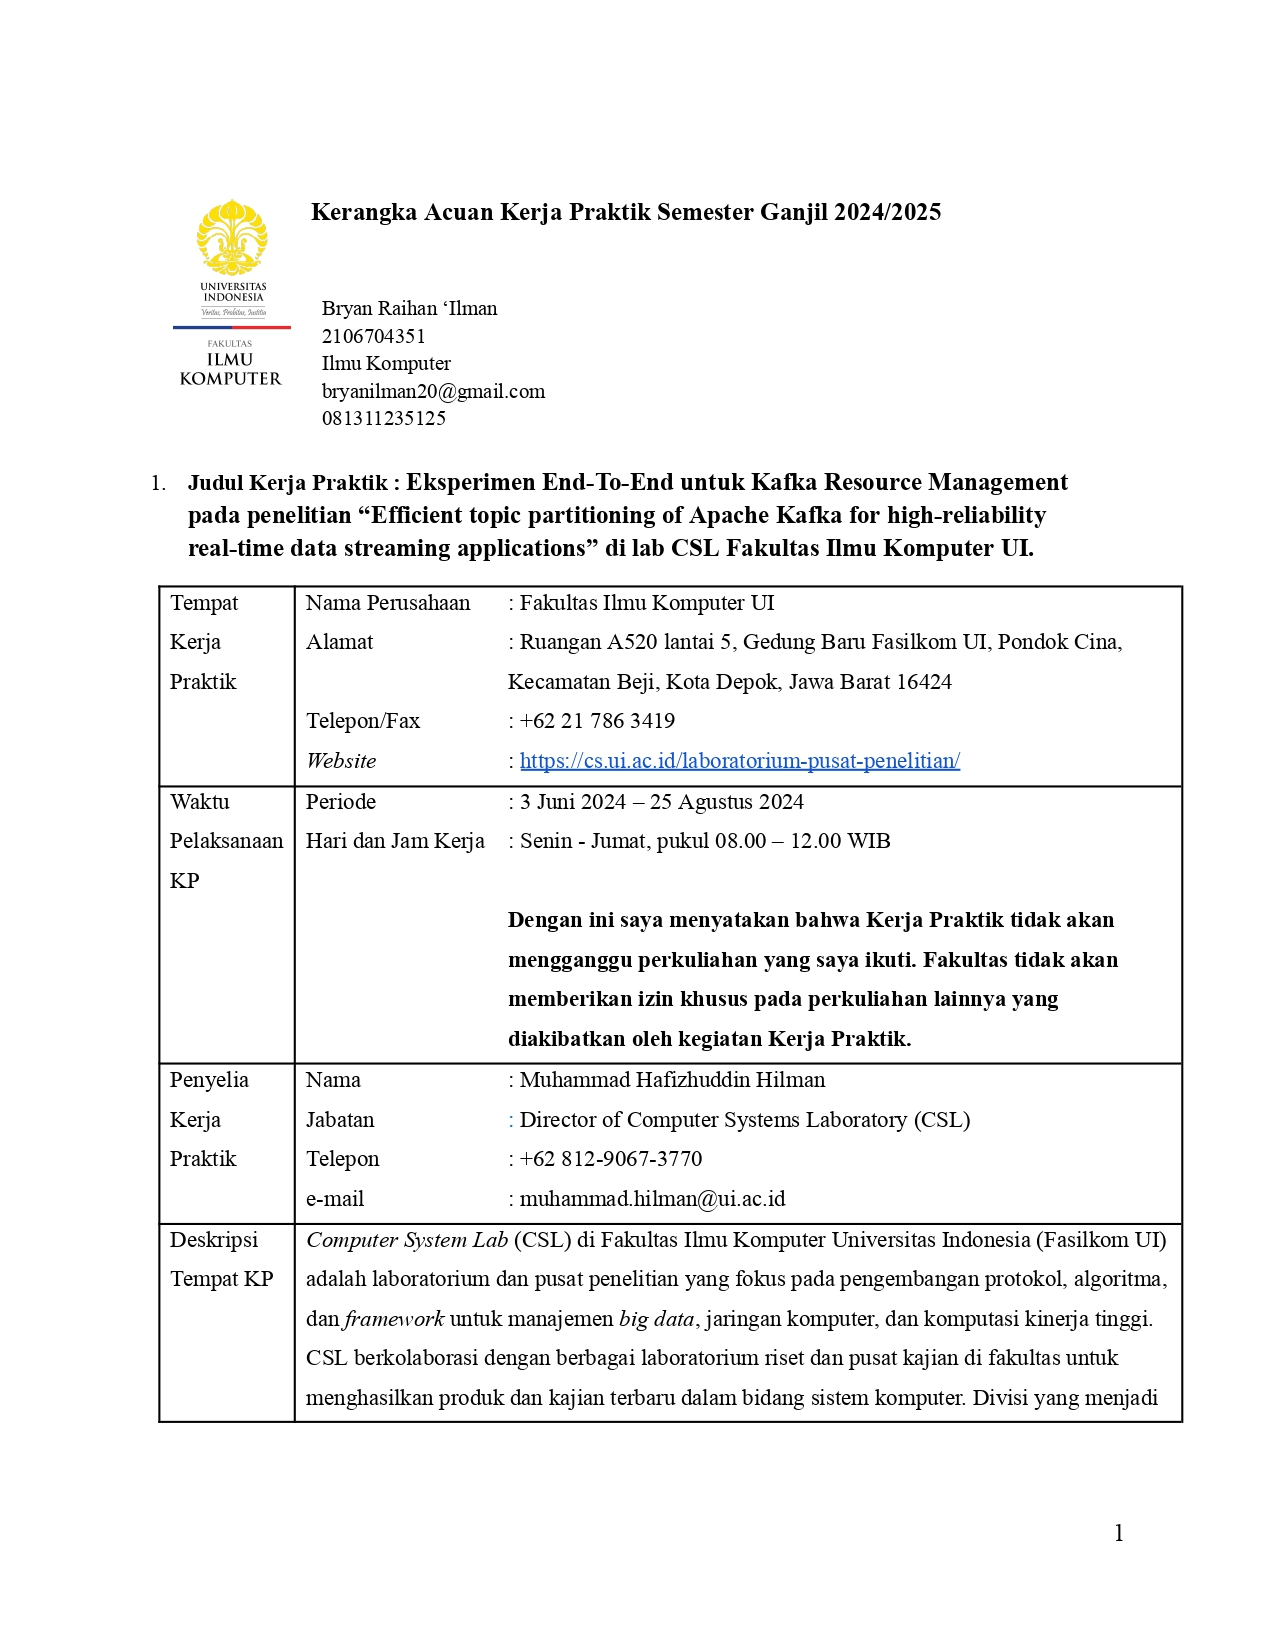
\includegraphics[width=1\textwidth]{assets/pics/KAKP_Bryan Raihan Ilman_2106704351_signed_page-0001.jpg}

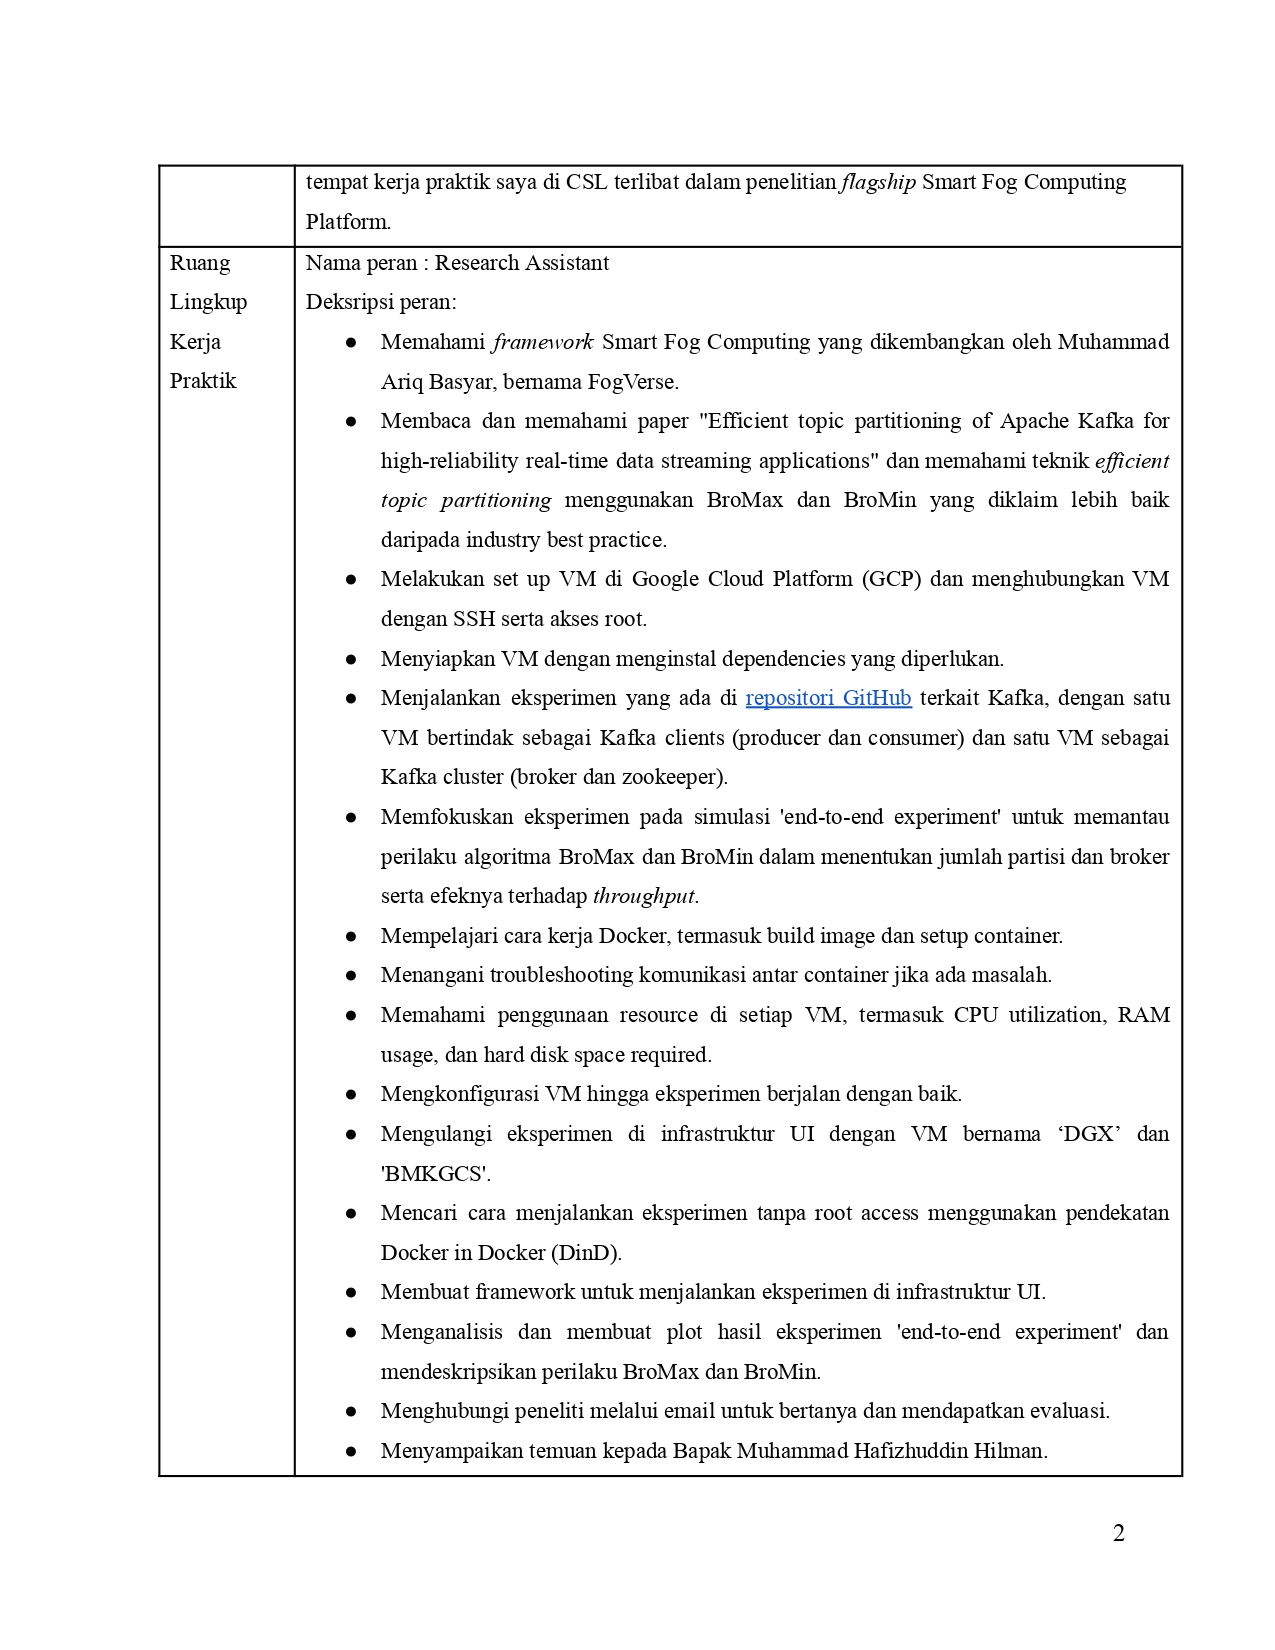
\includegraphics[width=1\textwidth]{assets/pics/KAKP_Bryan Raihan Ilman_2106704351_signed_page-0002.jpg}

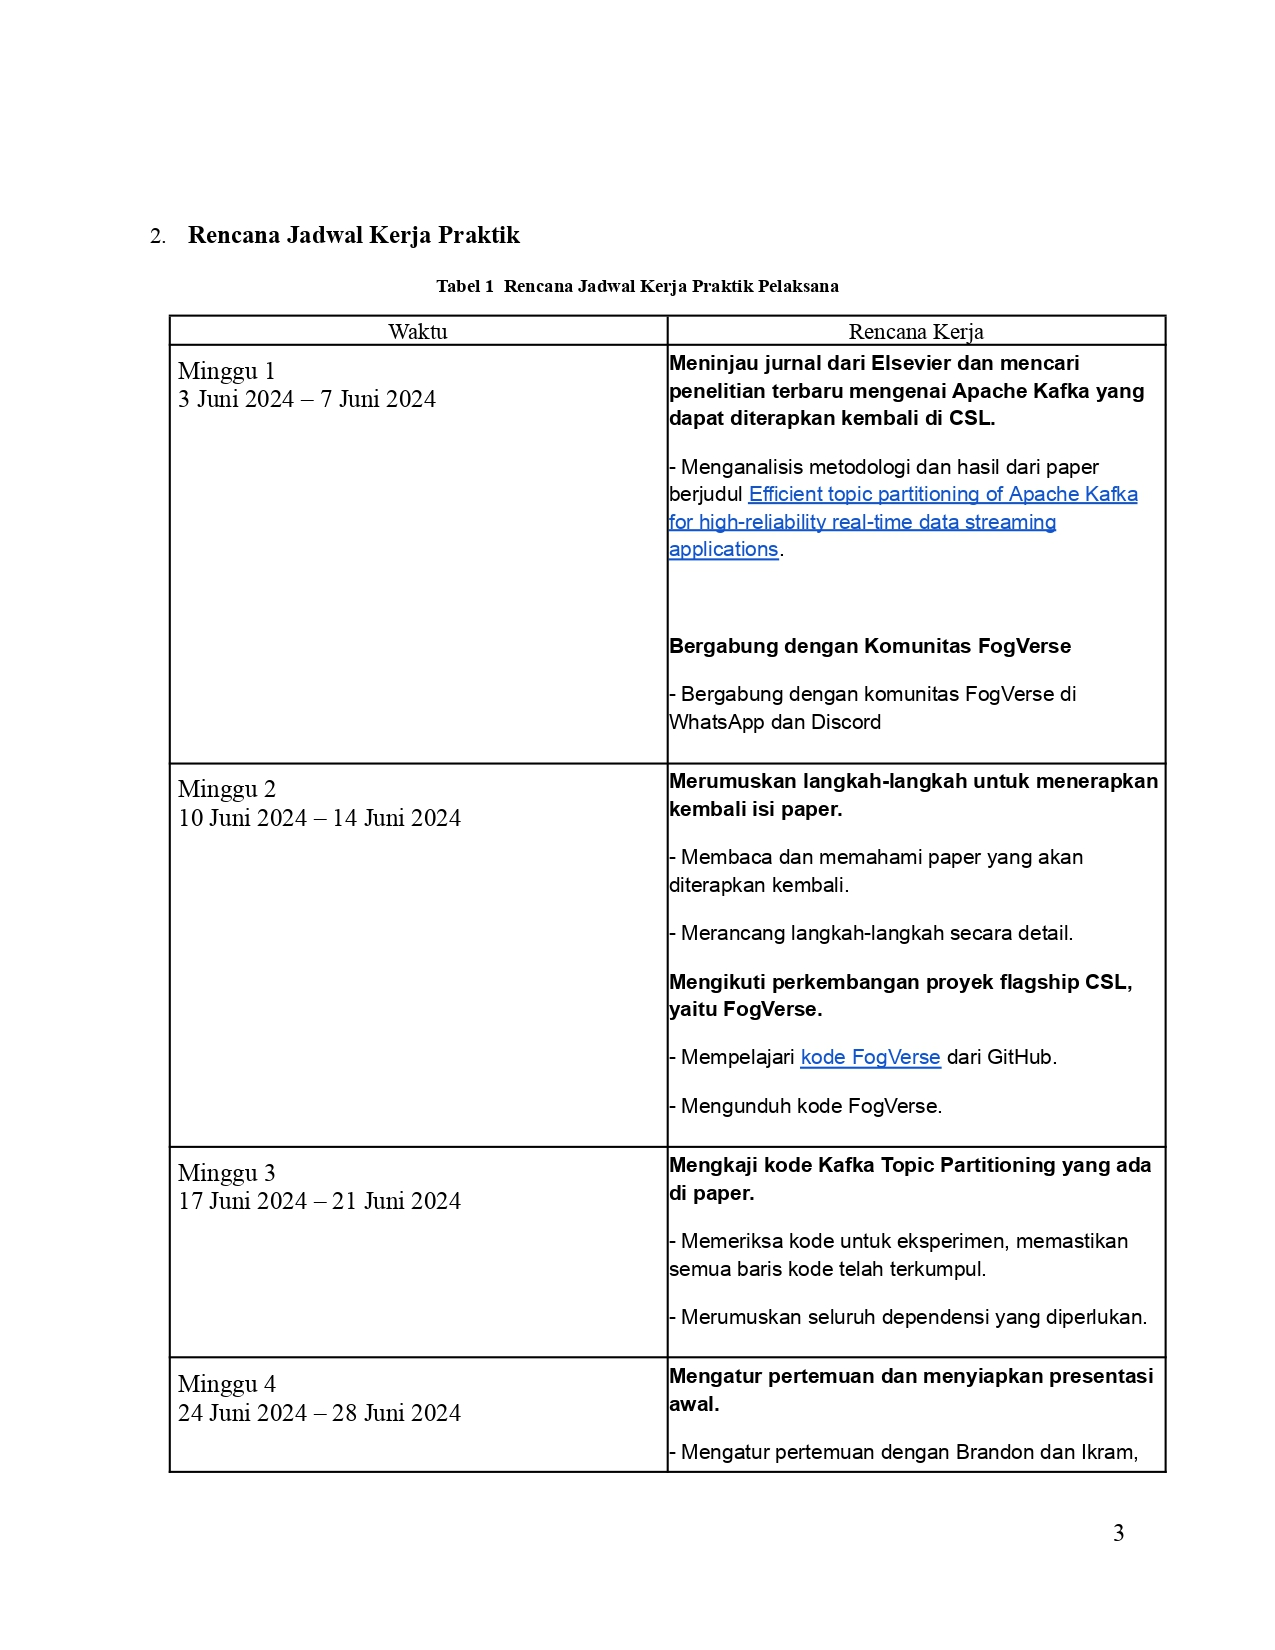
\includegraphics[width=1\textwidth]{assets/pics/KAKP_Bryan Raihan Ilman_2106704351_signed_page-0003.jpg}

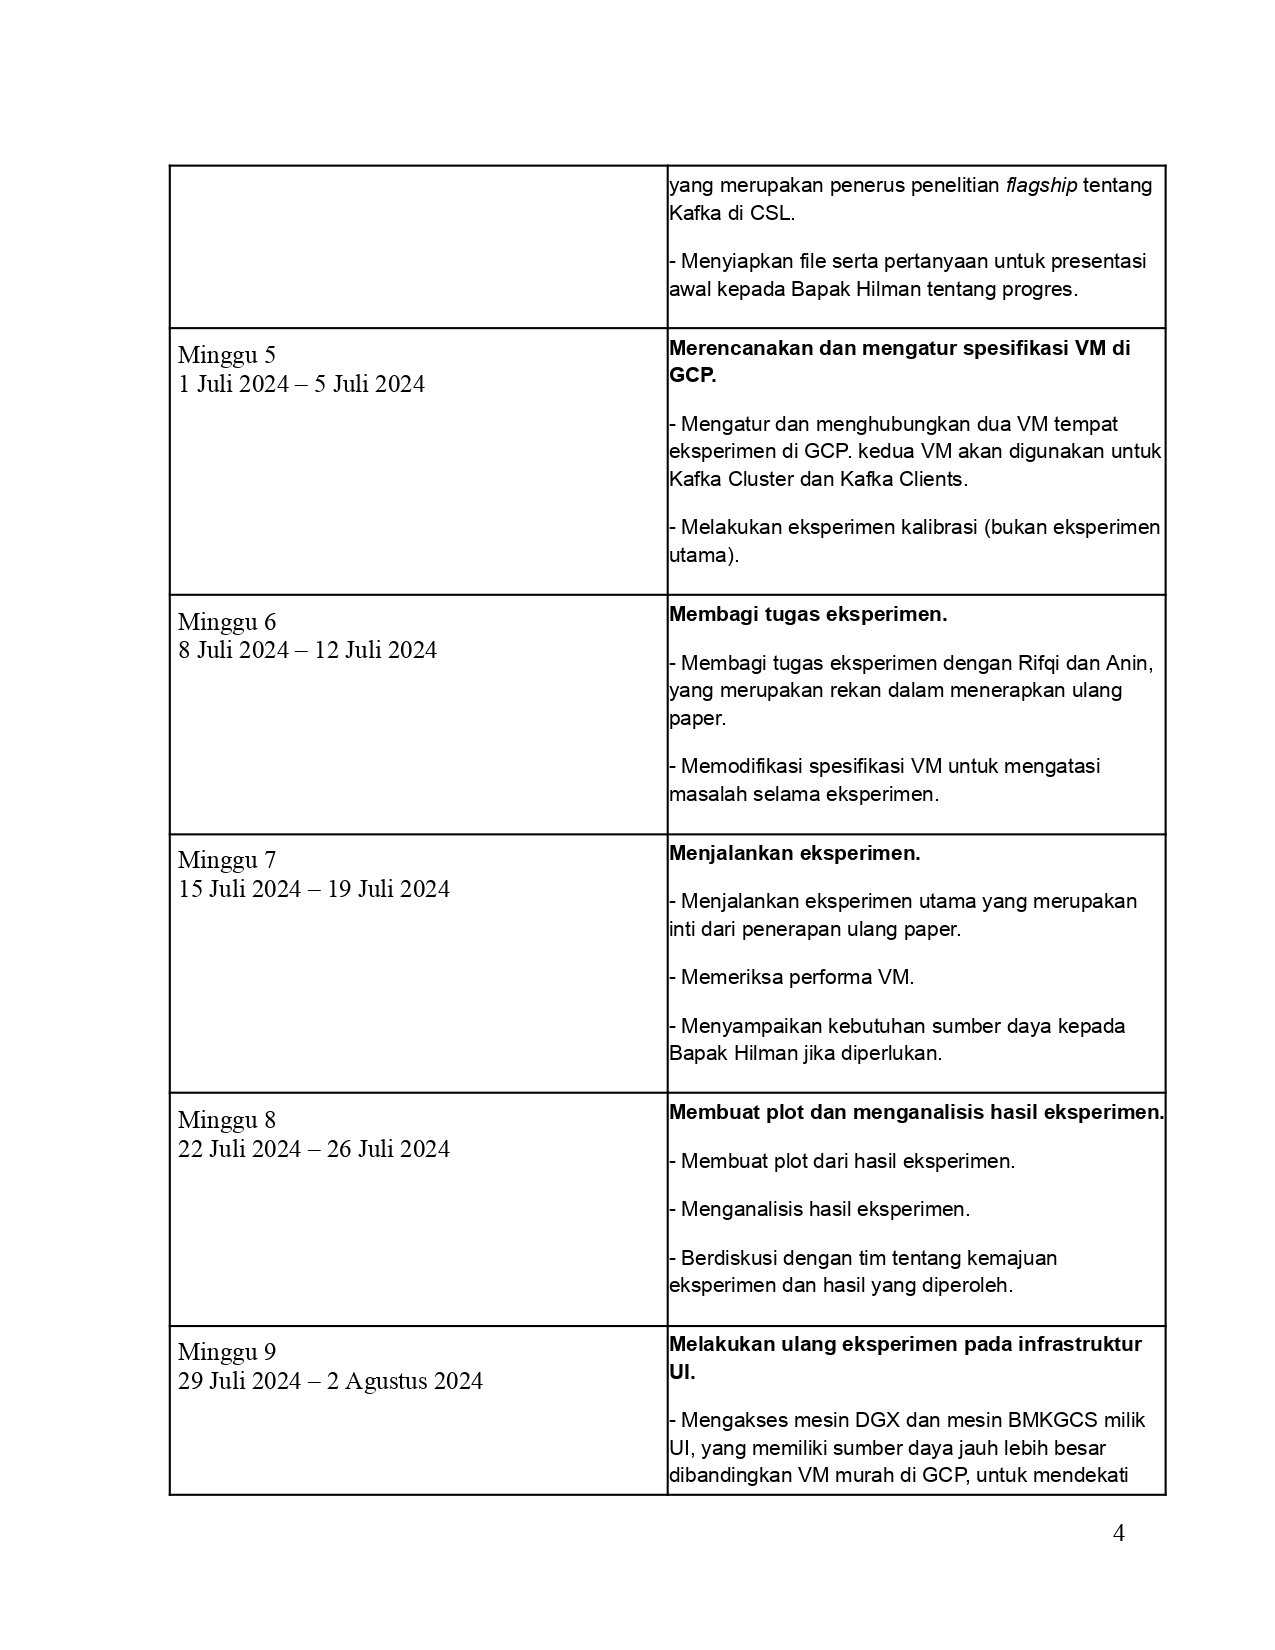
\includegraphics[width=1\textwidth]{assets/pics/KAKP_Bryan Raihan Ilman_2106704351_signed_page-0004.jpg}

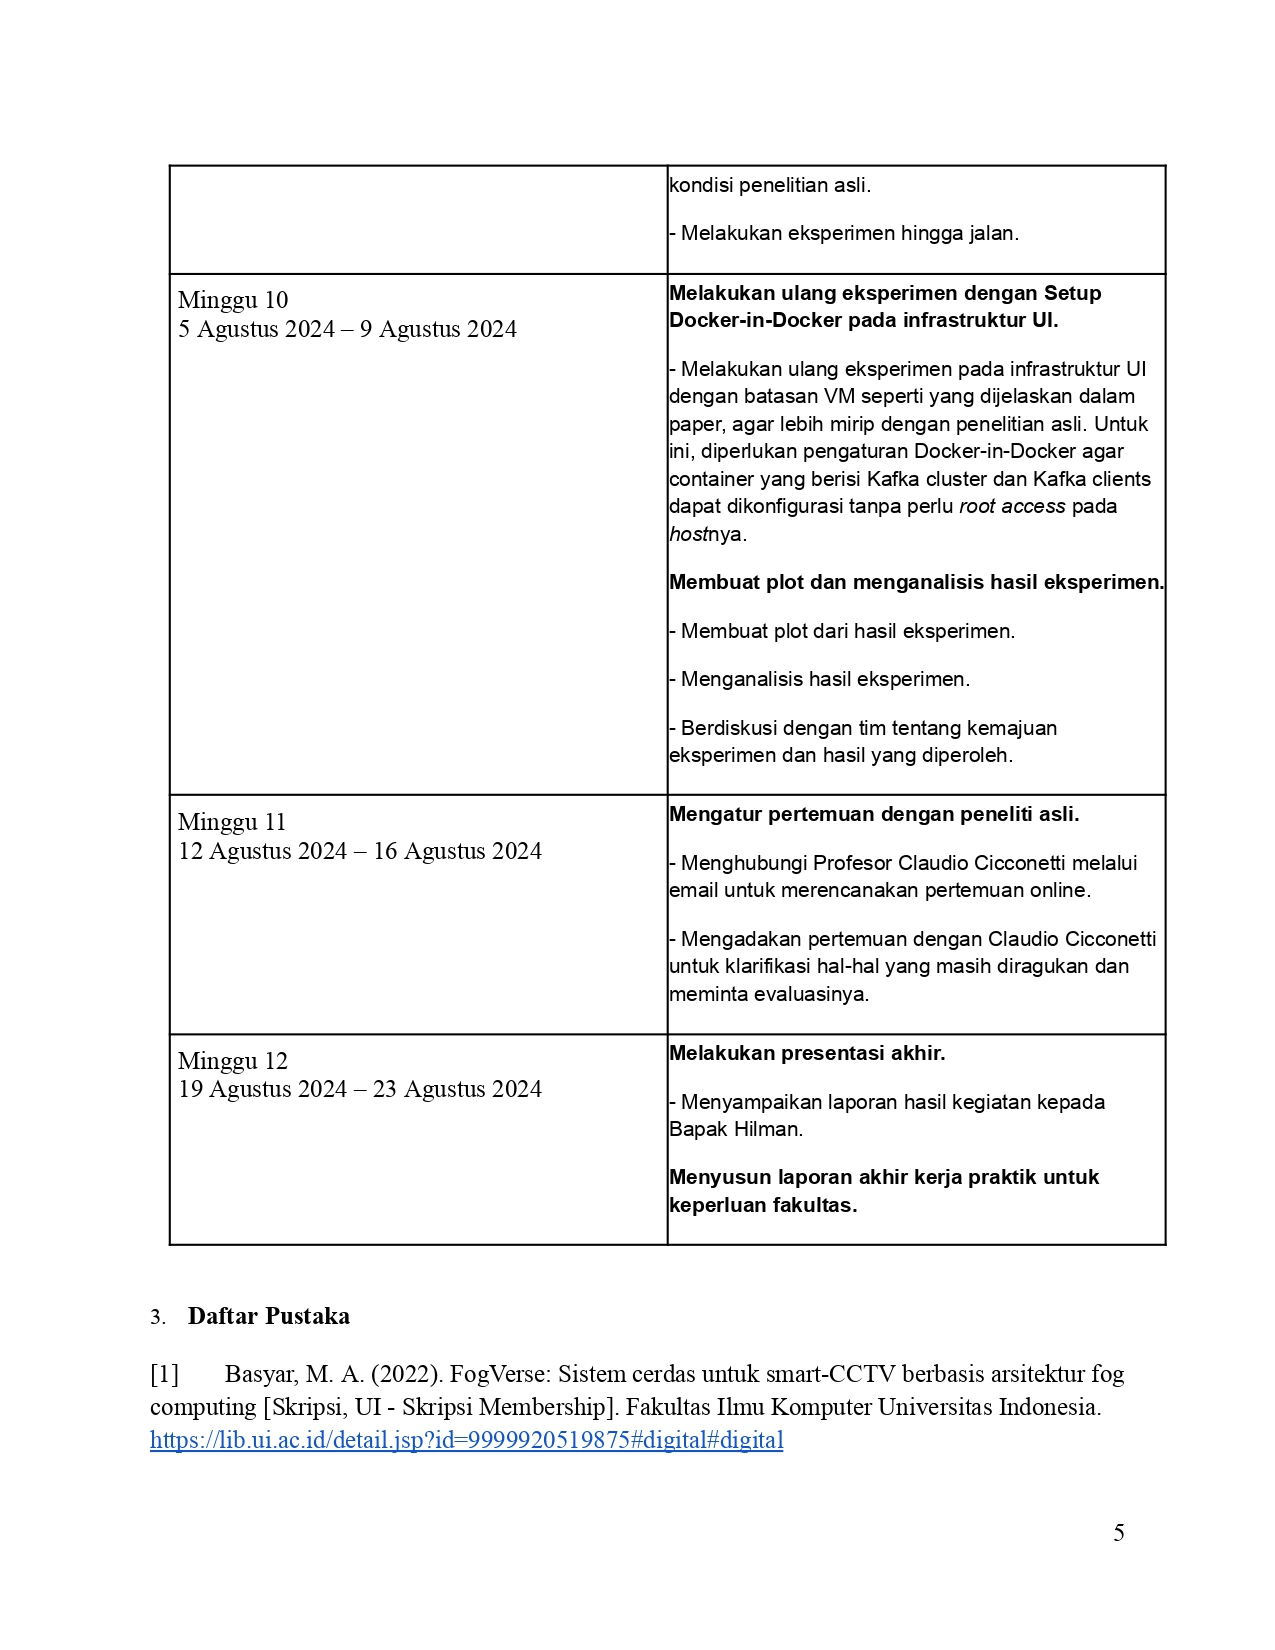
\includegraphics[width=1\textwidth]{assets/pics/KAKP_Bryan Raihan Ilman_2106704351_signed_page-0005.jpg}

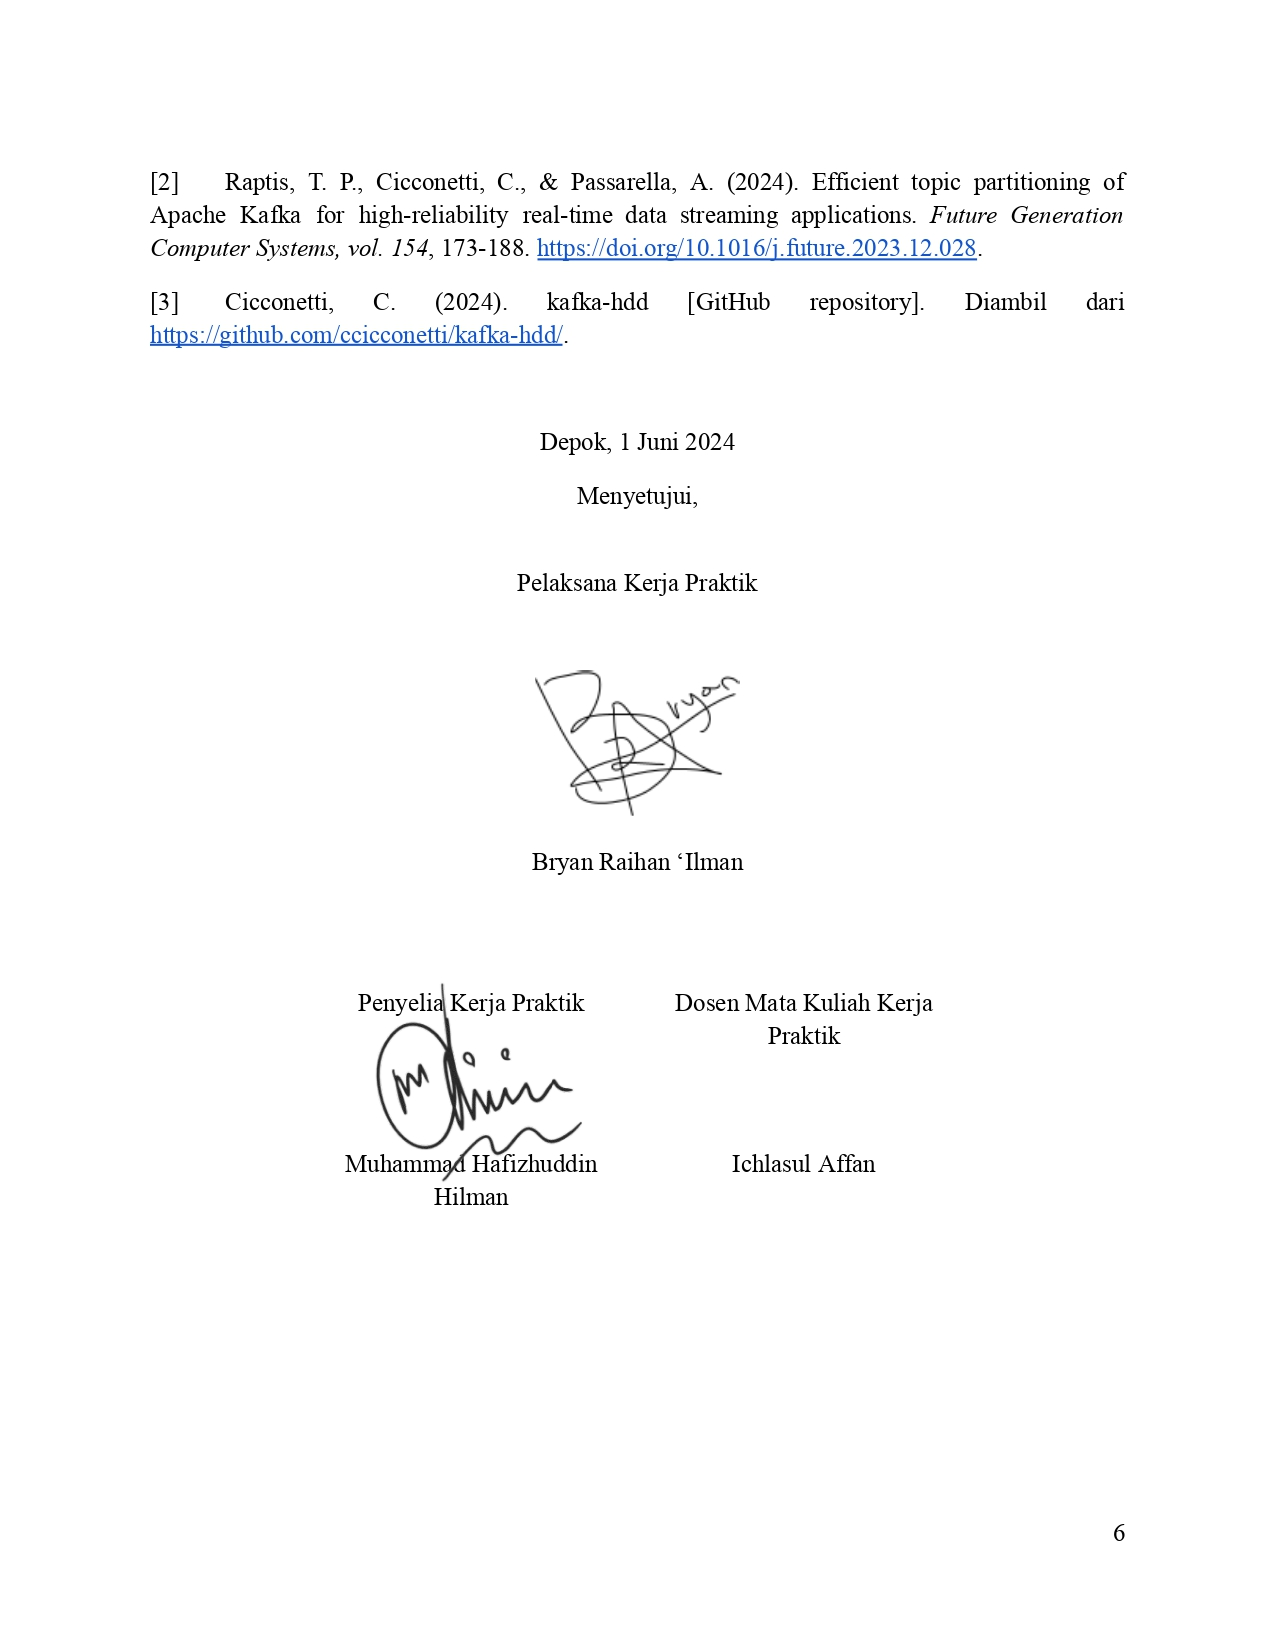
\includegraphics[width=1\textwidth]{assets/pics/KAKP_Bryan Raihan Ilman_2106704351_signed_page-0006.jpg}

\begin{center}
    \textbf{\large LAMPIRAN 2: LOG KERJA PRAKTIK}
\end{center}

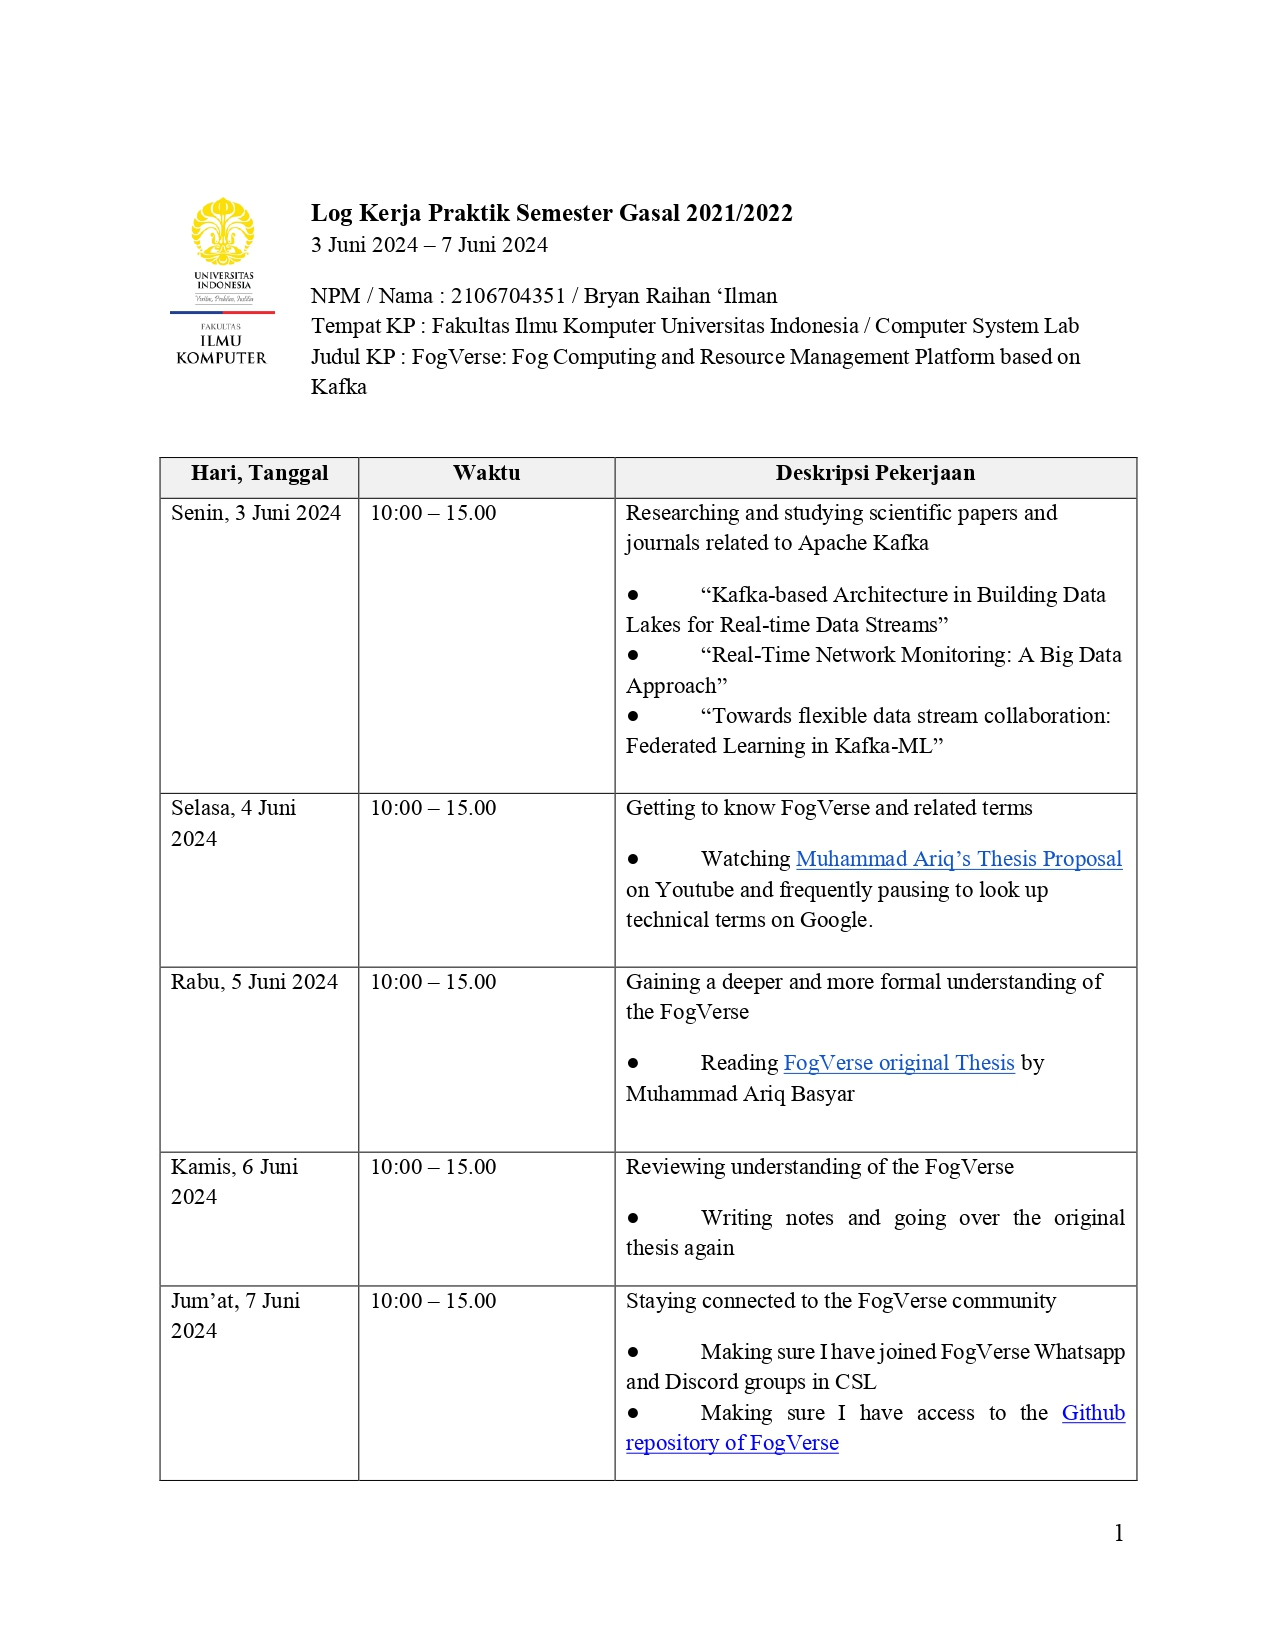
\includegraphics[width=1\textwidth]{assets/pics/Log-1-CSL-Bryan Raihan Ilman-0001.jpg}

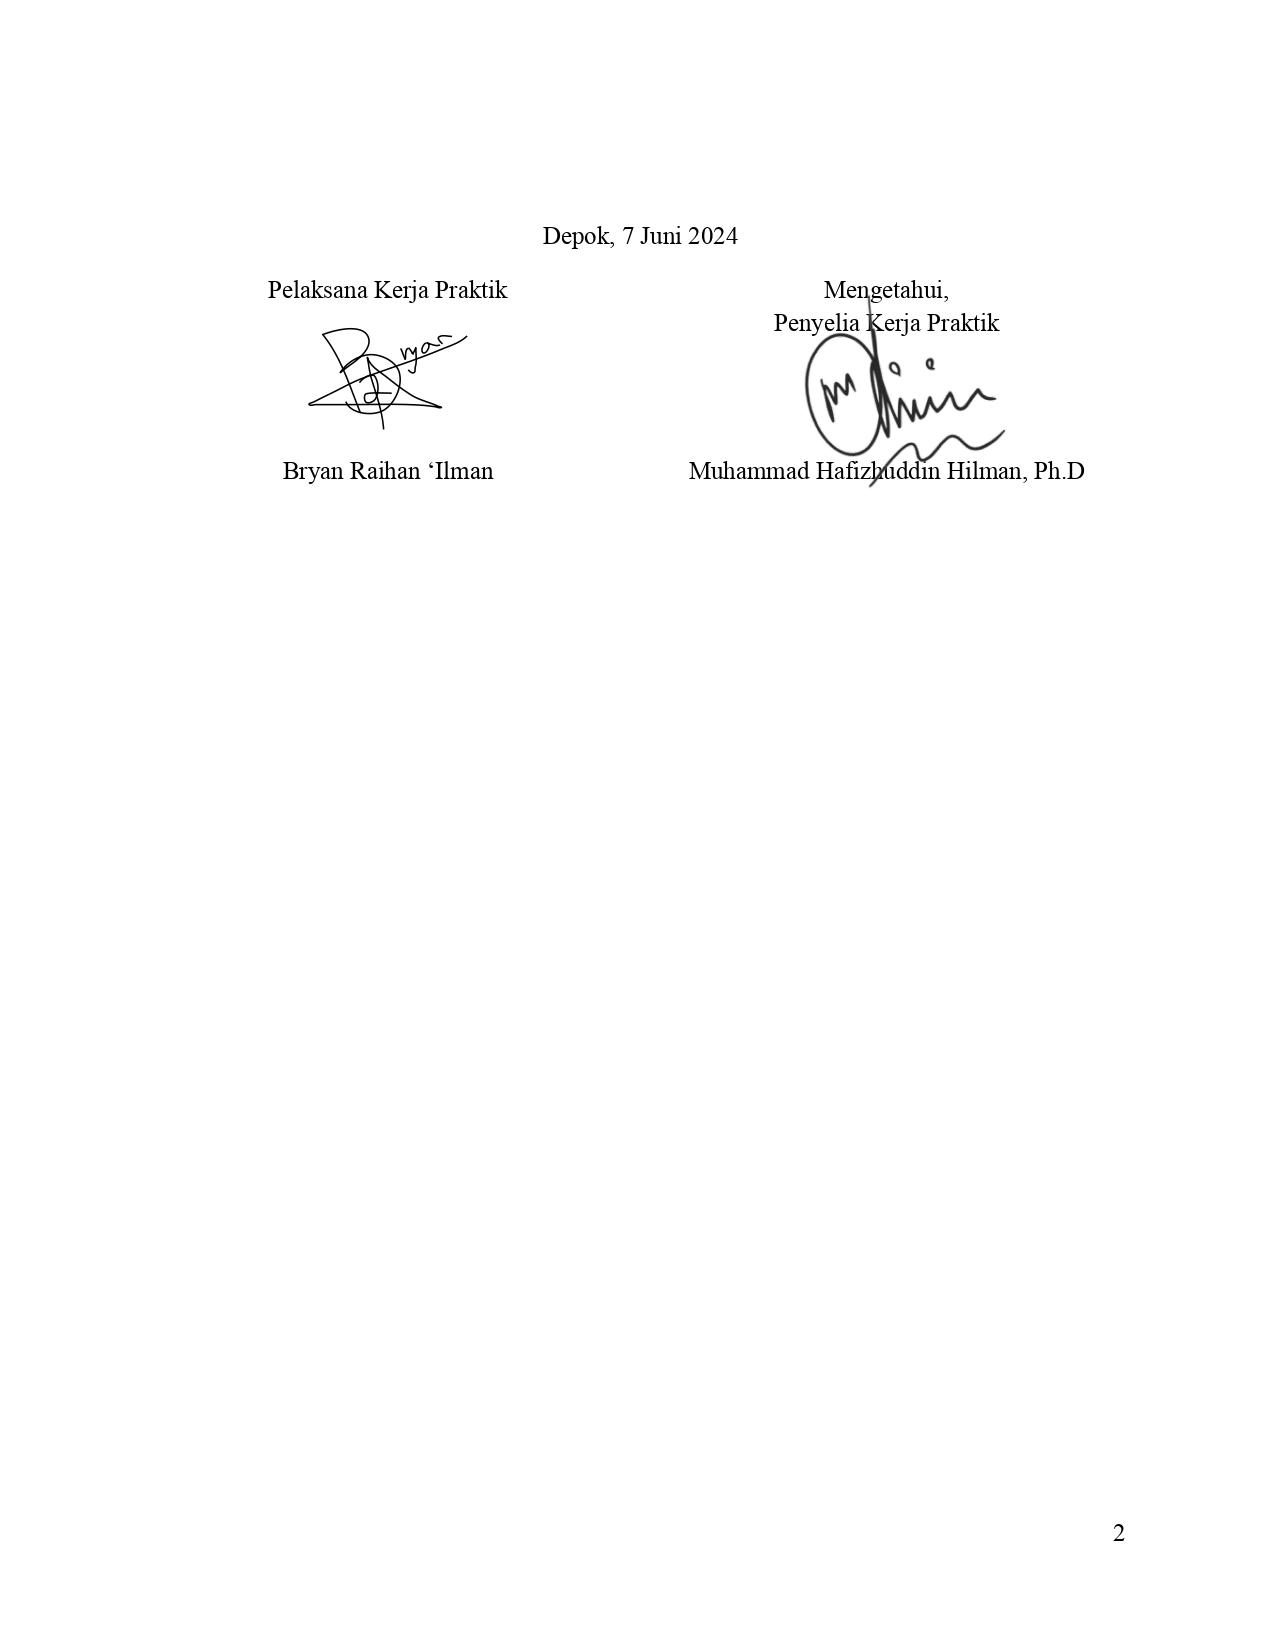
\includegraphics[width=1\textwidth]{assets/pics/Log-1-CSL-Bryan Raihan Ilman-0002.jpg}

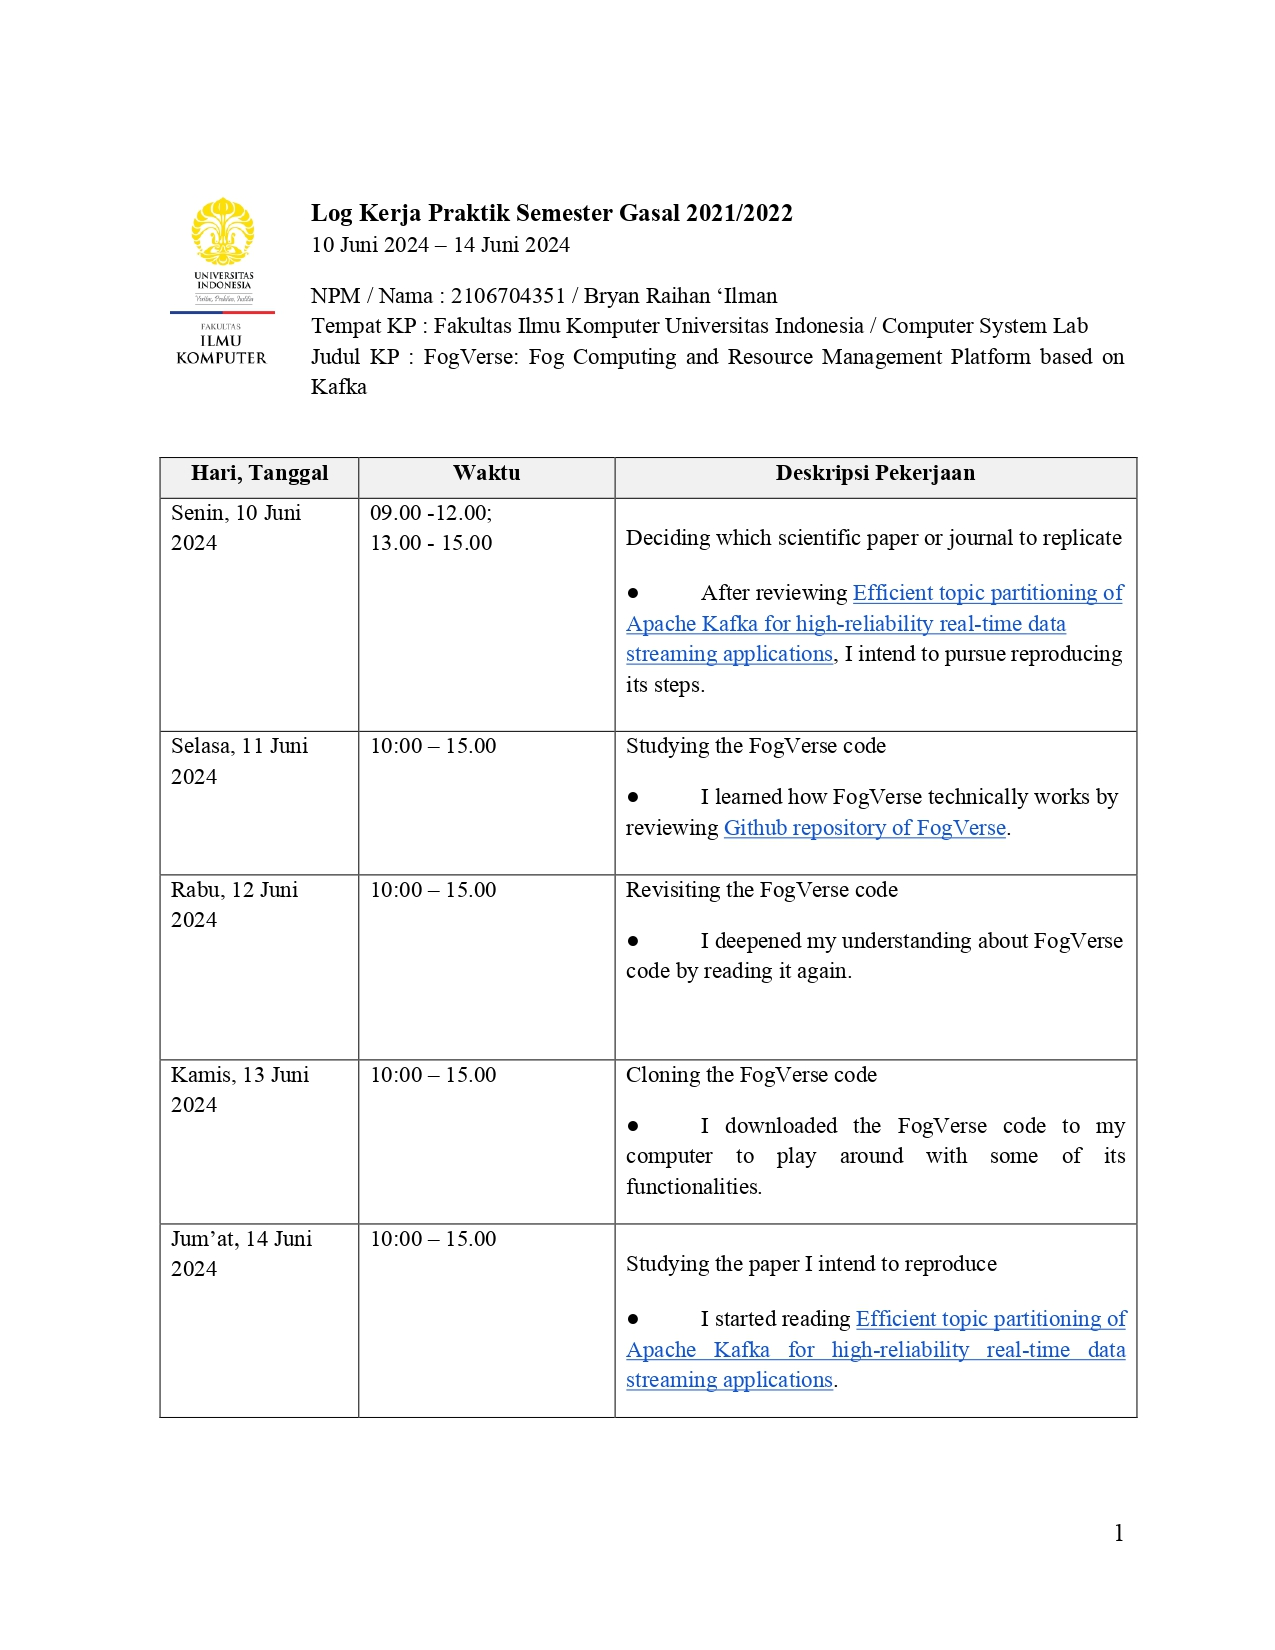
\includegraphics[width=1\textwidth]{assets/pics/Log-2-CSL-Bryan Raihan Ilman-0001.jpg}

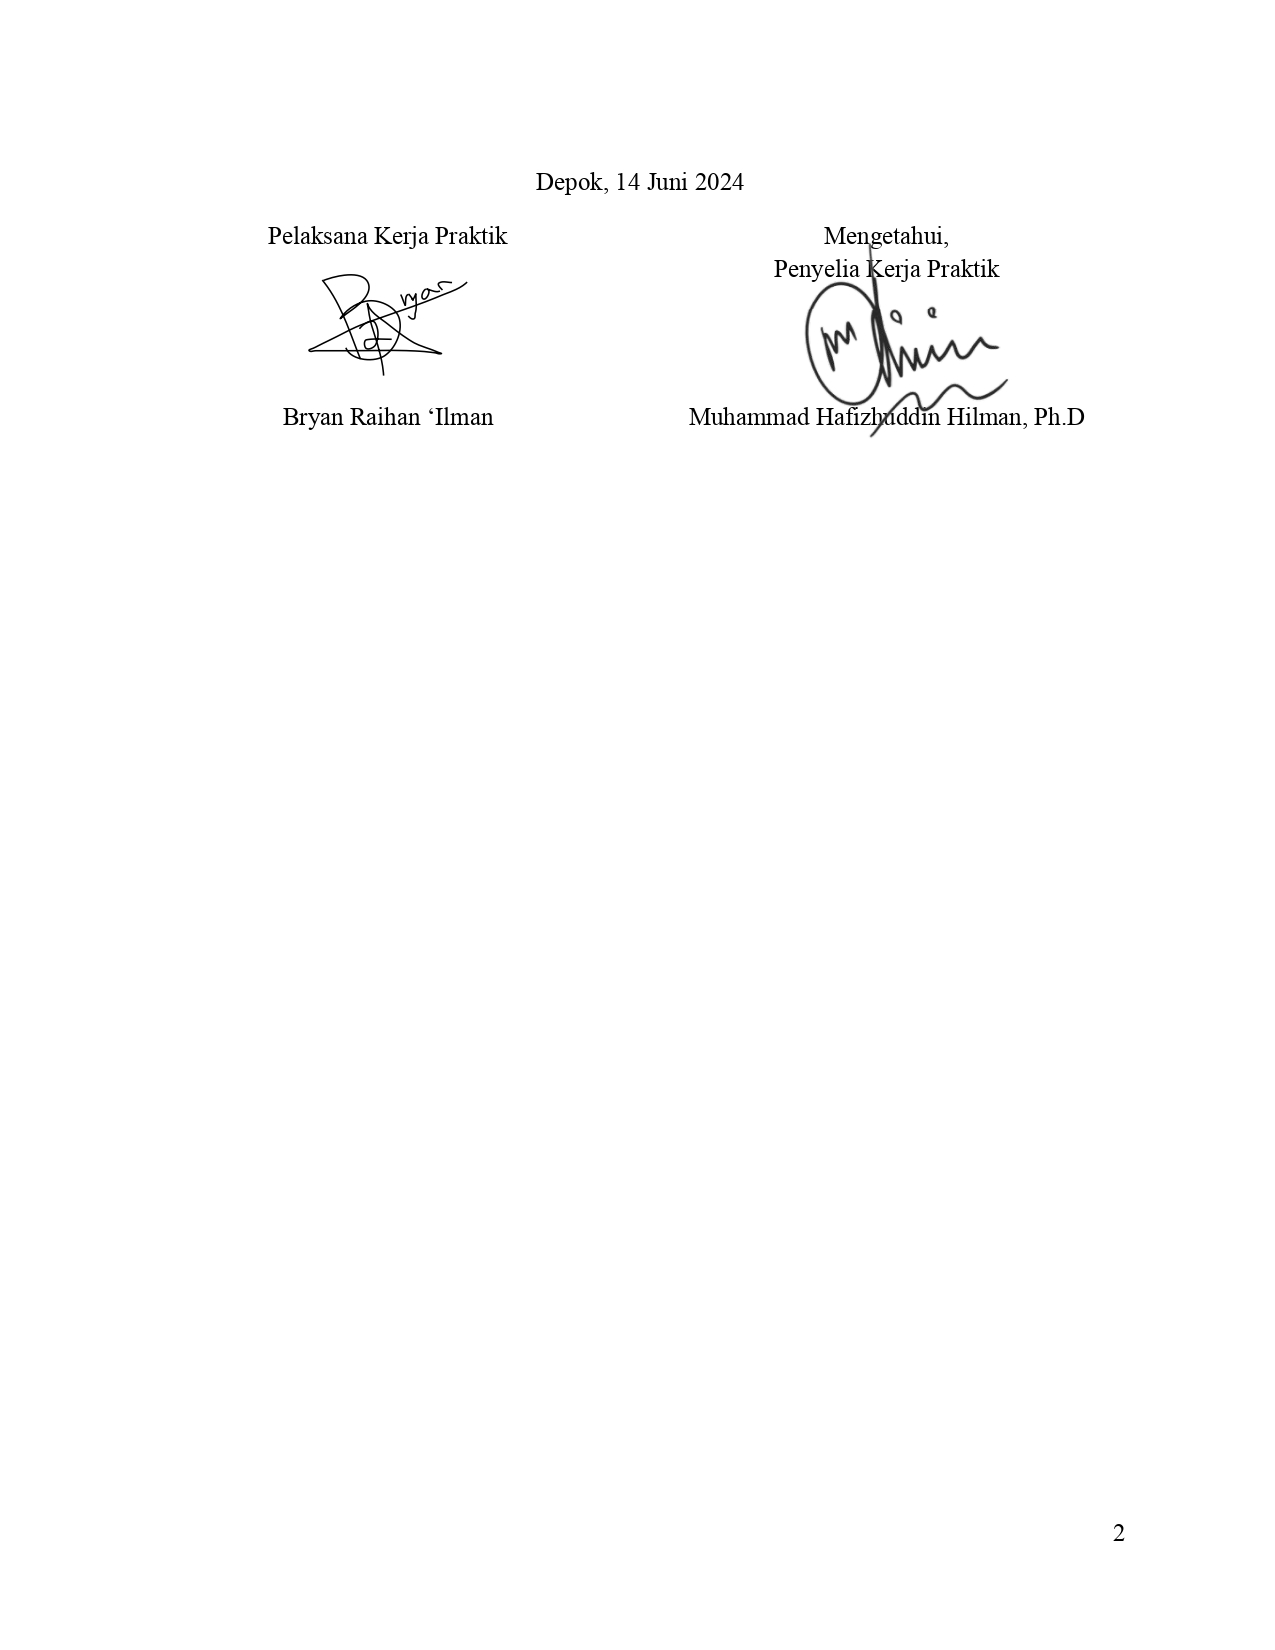
\includegraphics[width=1\textwidth]{assets/pics/Log-2-CSL-Bryan Raihan Ilman-0002.jpg}

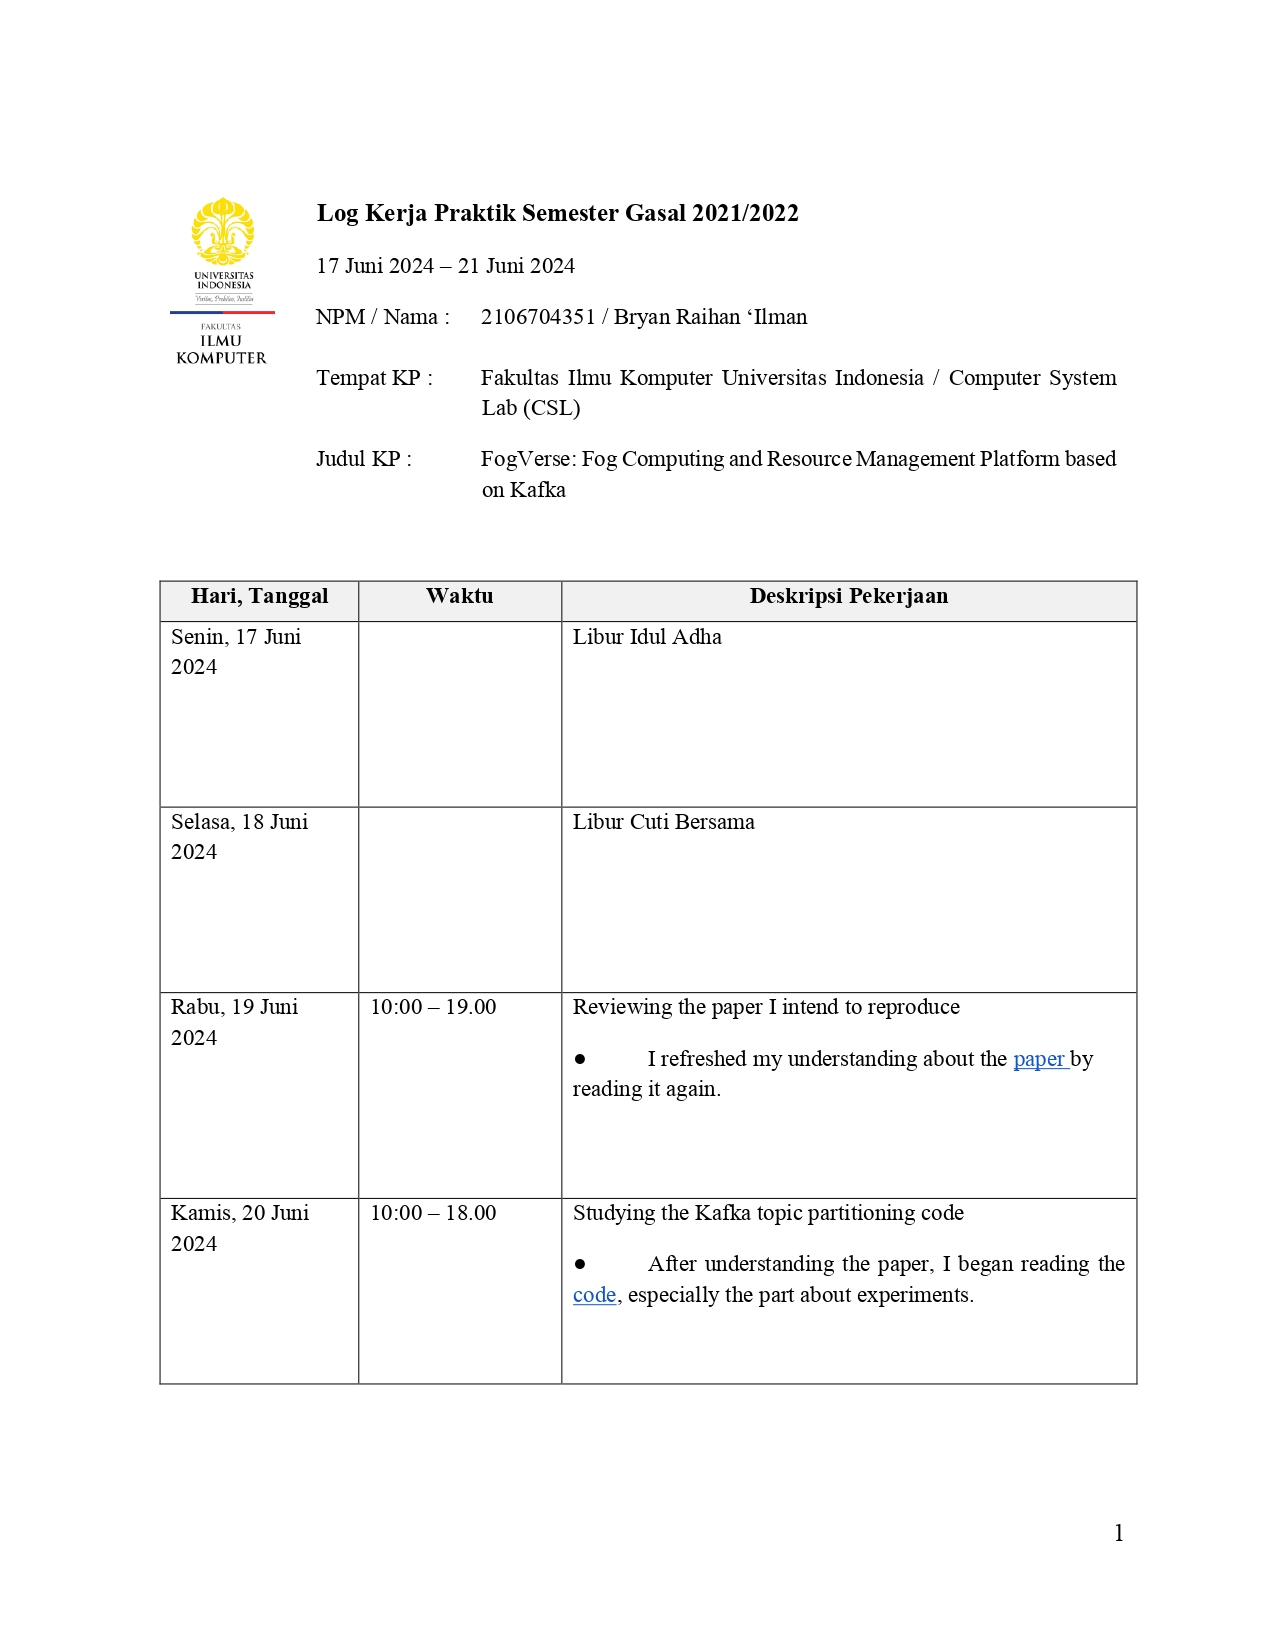
\includegraphics[width=1\textwidth]{assets/pics/Log-3-CSL-Bryan Raihan Ilman-0001.jpg}

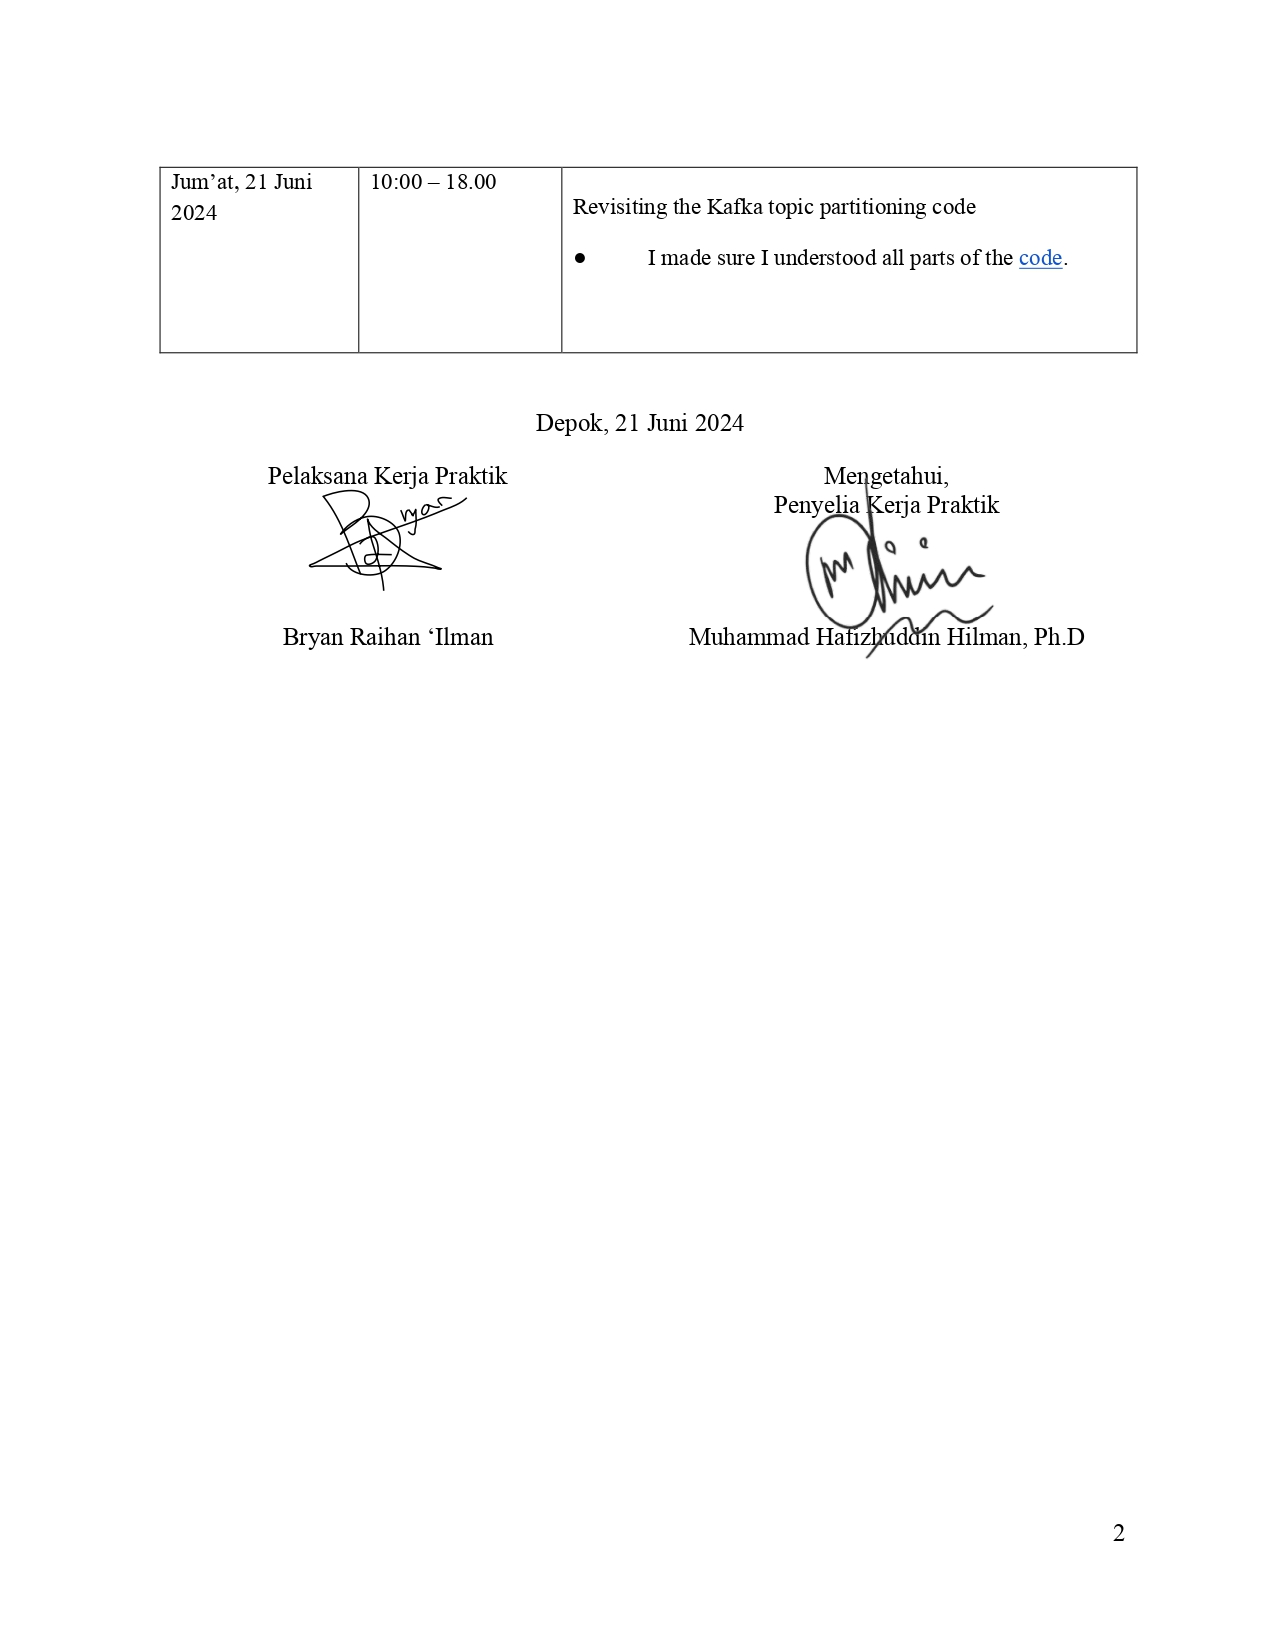
\includegraphics[width=1\textwidth]{assets/pics/Log-3-CSL-Bryan Raihan Ilman-0002.jpg}

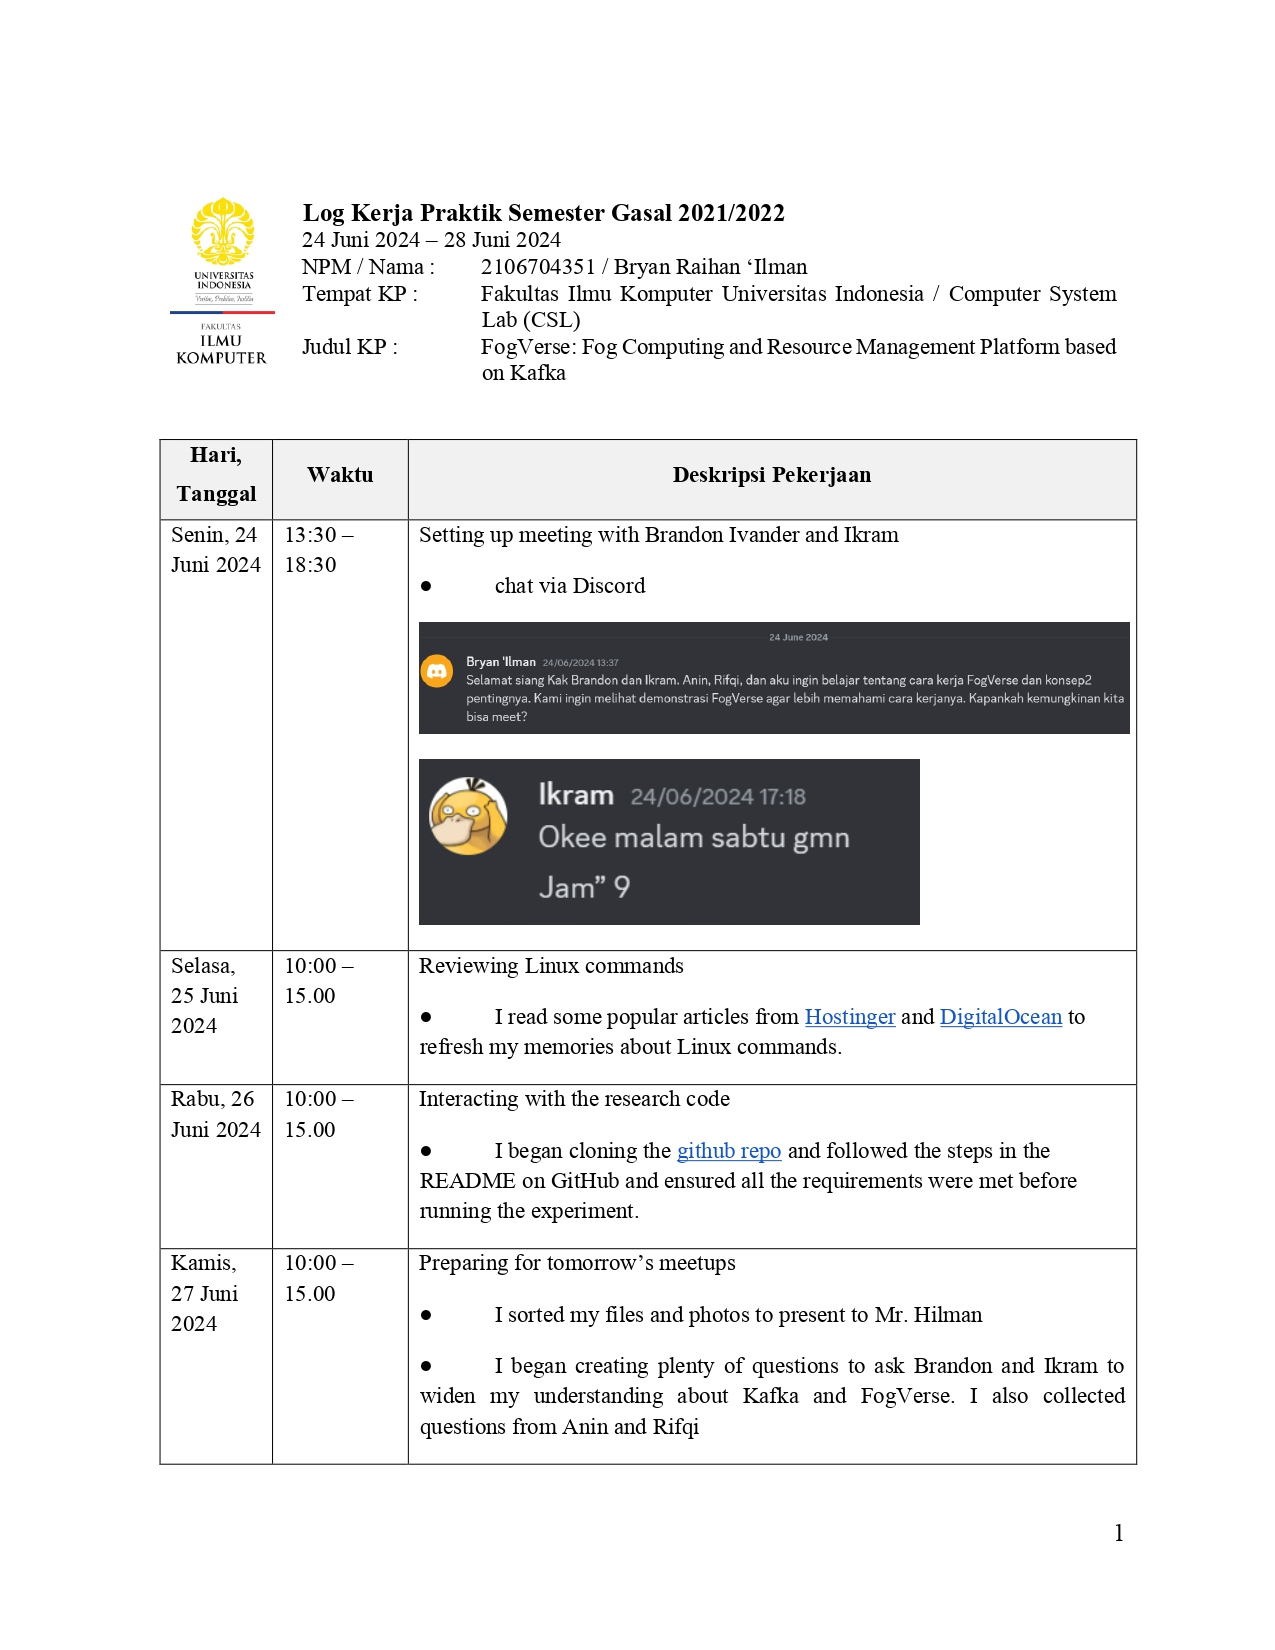
\includegraphics[width=1\textwidth]{assets/pics/Log-4-CSL-Bryan Raihan Ilman-0001.jpg}

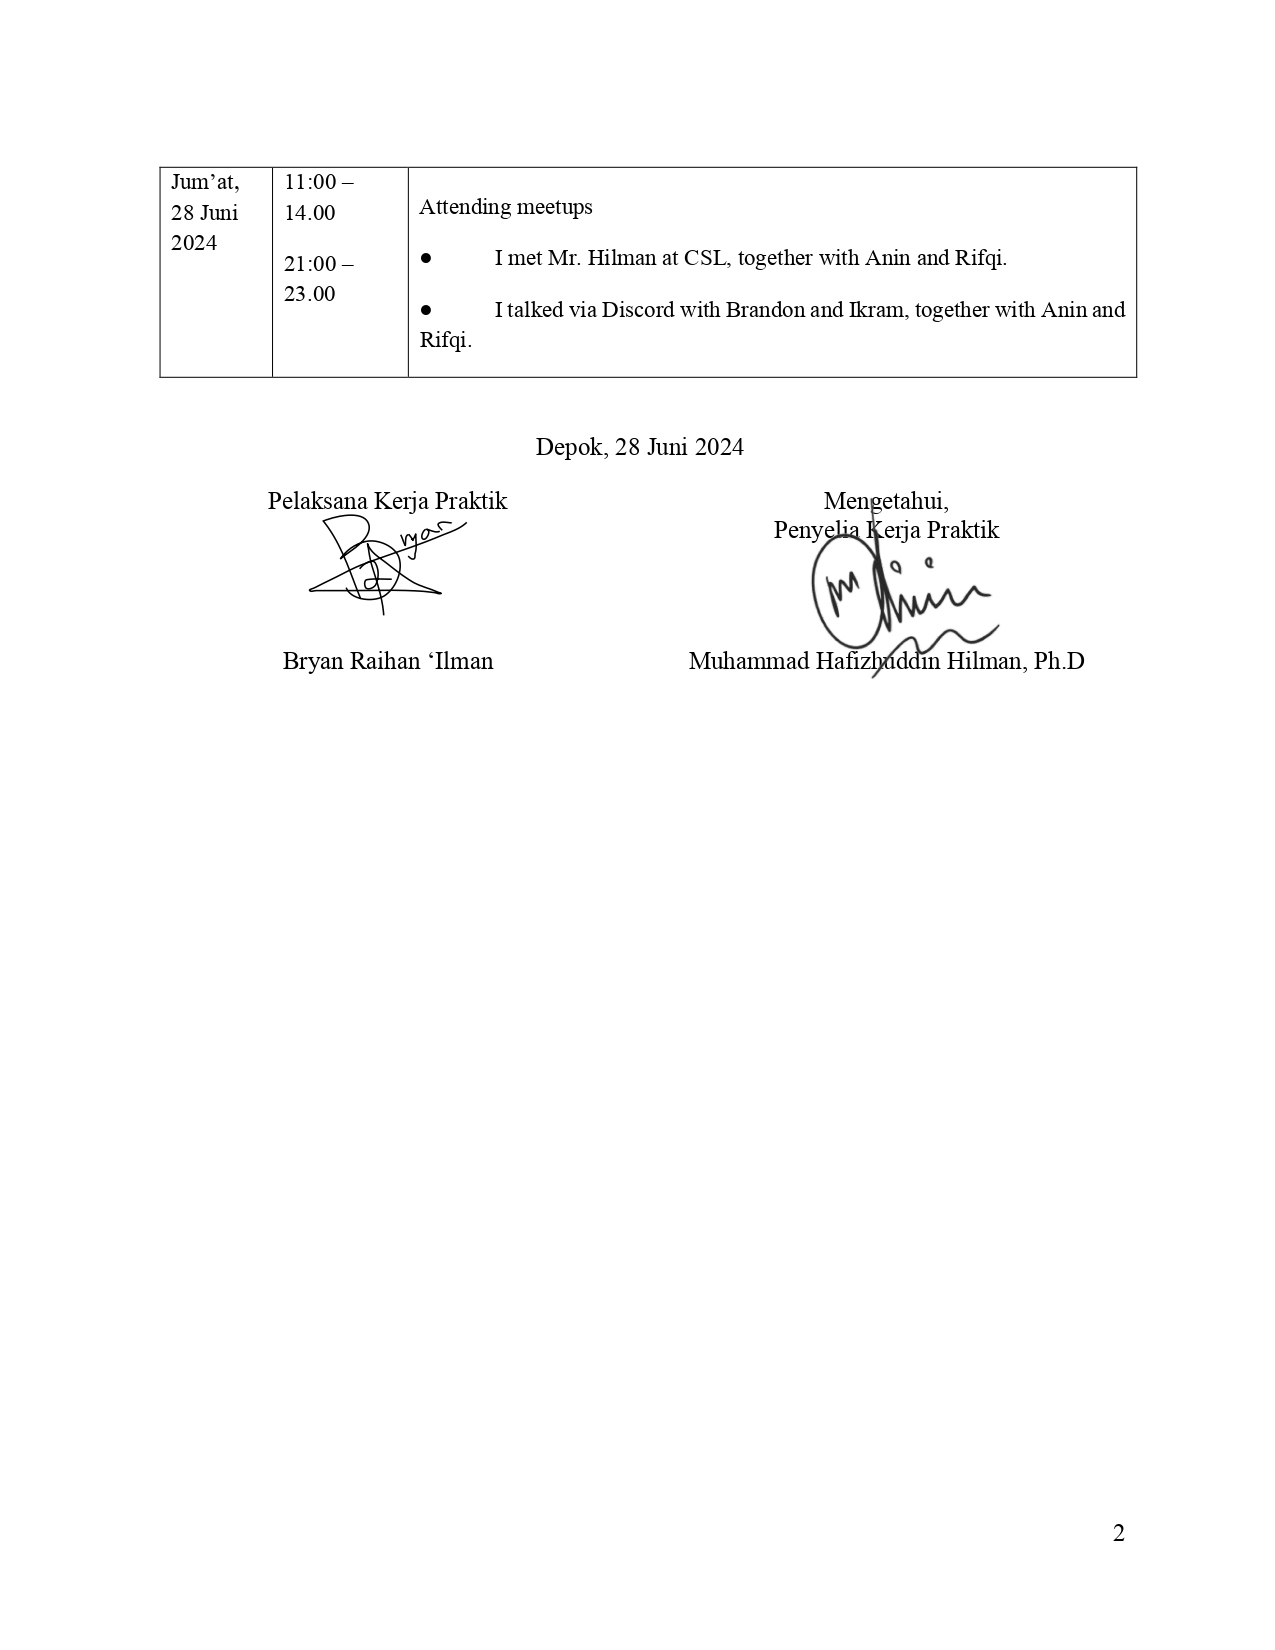
\includegraphics[width=1\textwidth]{assets/pics/Log-4-CSL-Bryan Raihan Ilman-0002.jpg}

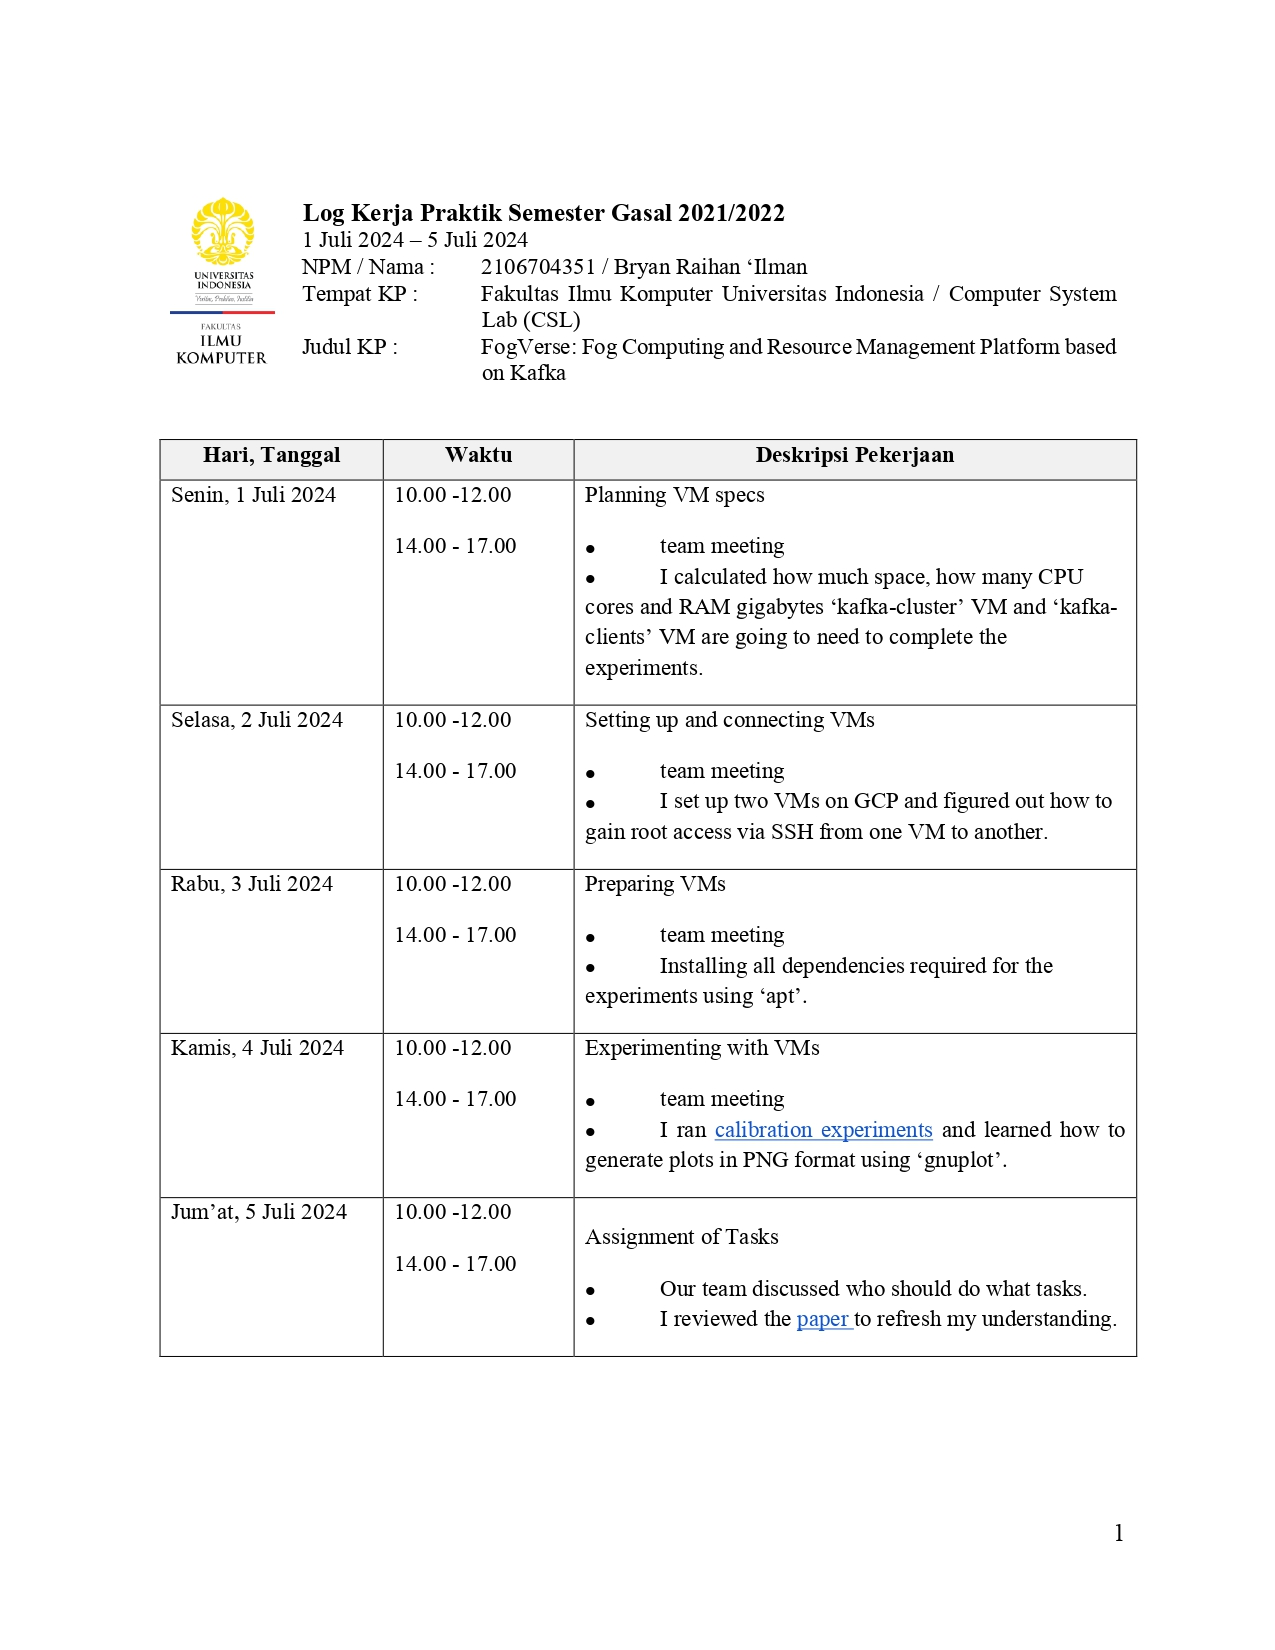
\includegraphics[width=1\textwidth]{assets/pics/Log-5-CSL-Bryan Raihan Ilman-0001.jpg}

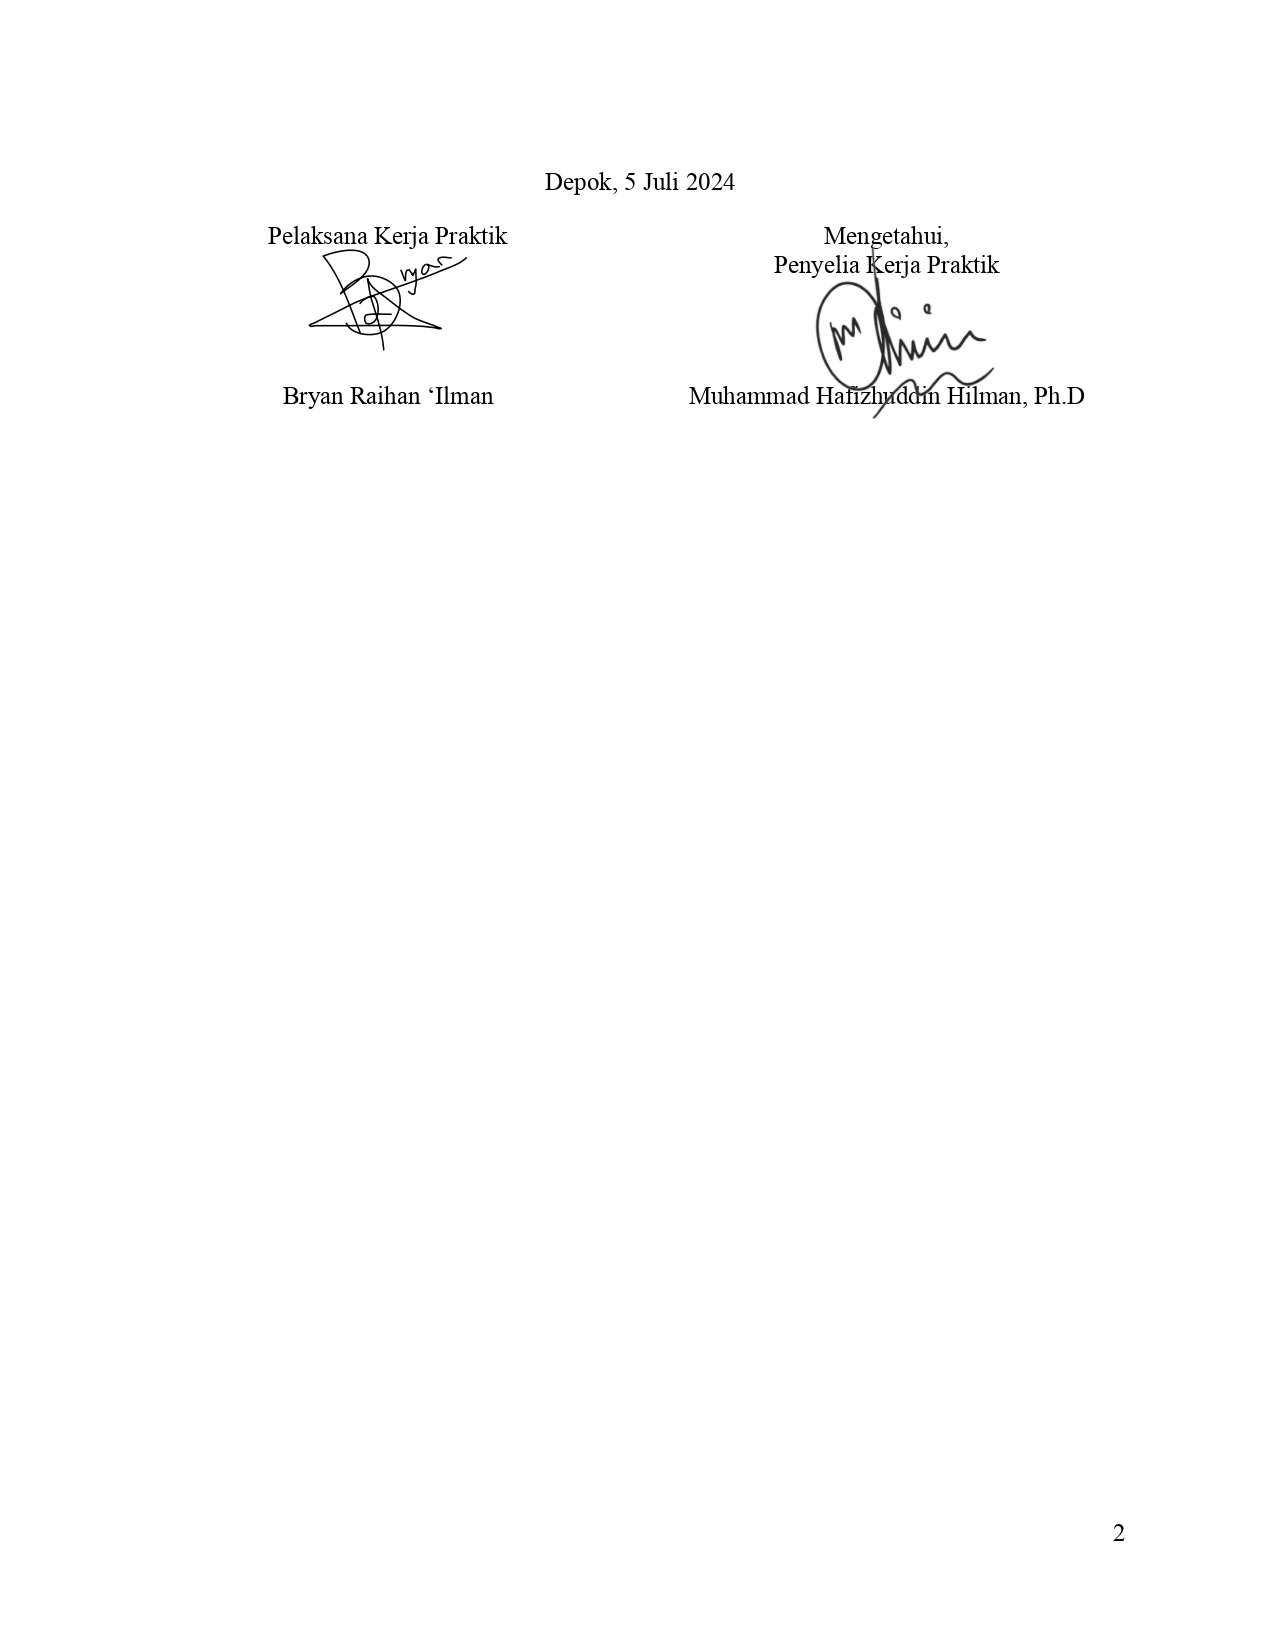
\includegraphics[width=1\textwidth]{assets/pics/Log-5-CSL-Bryan Raihan Ilman-0002.jpg}

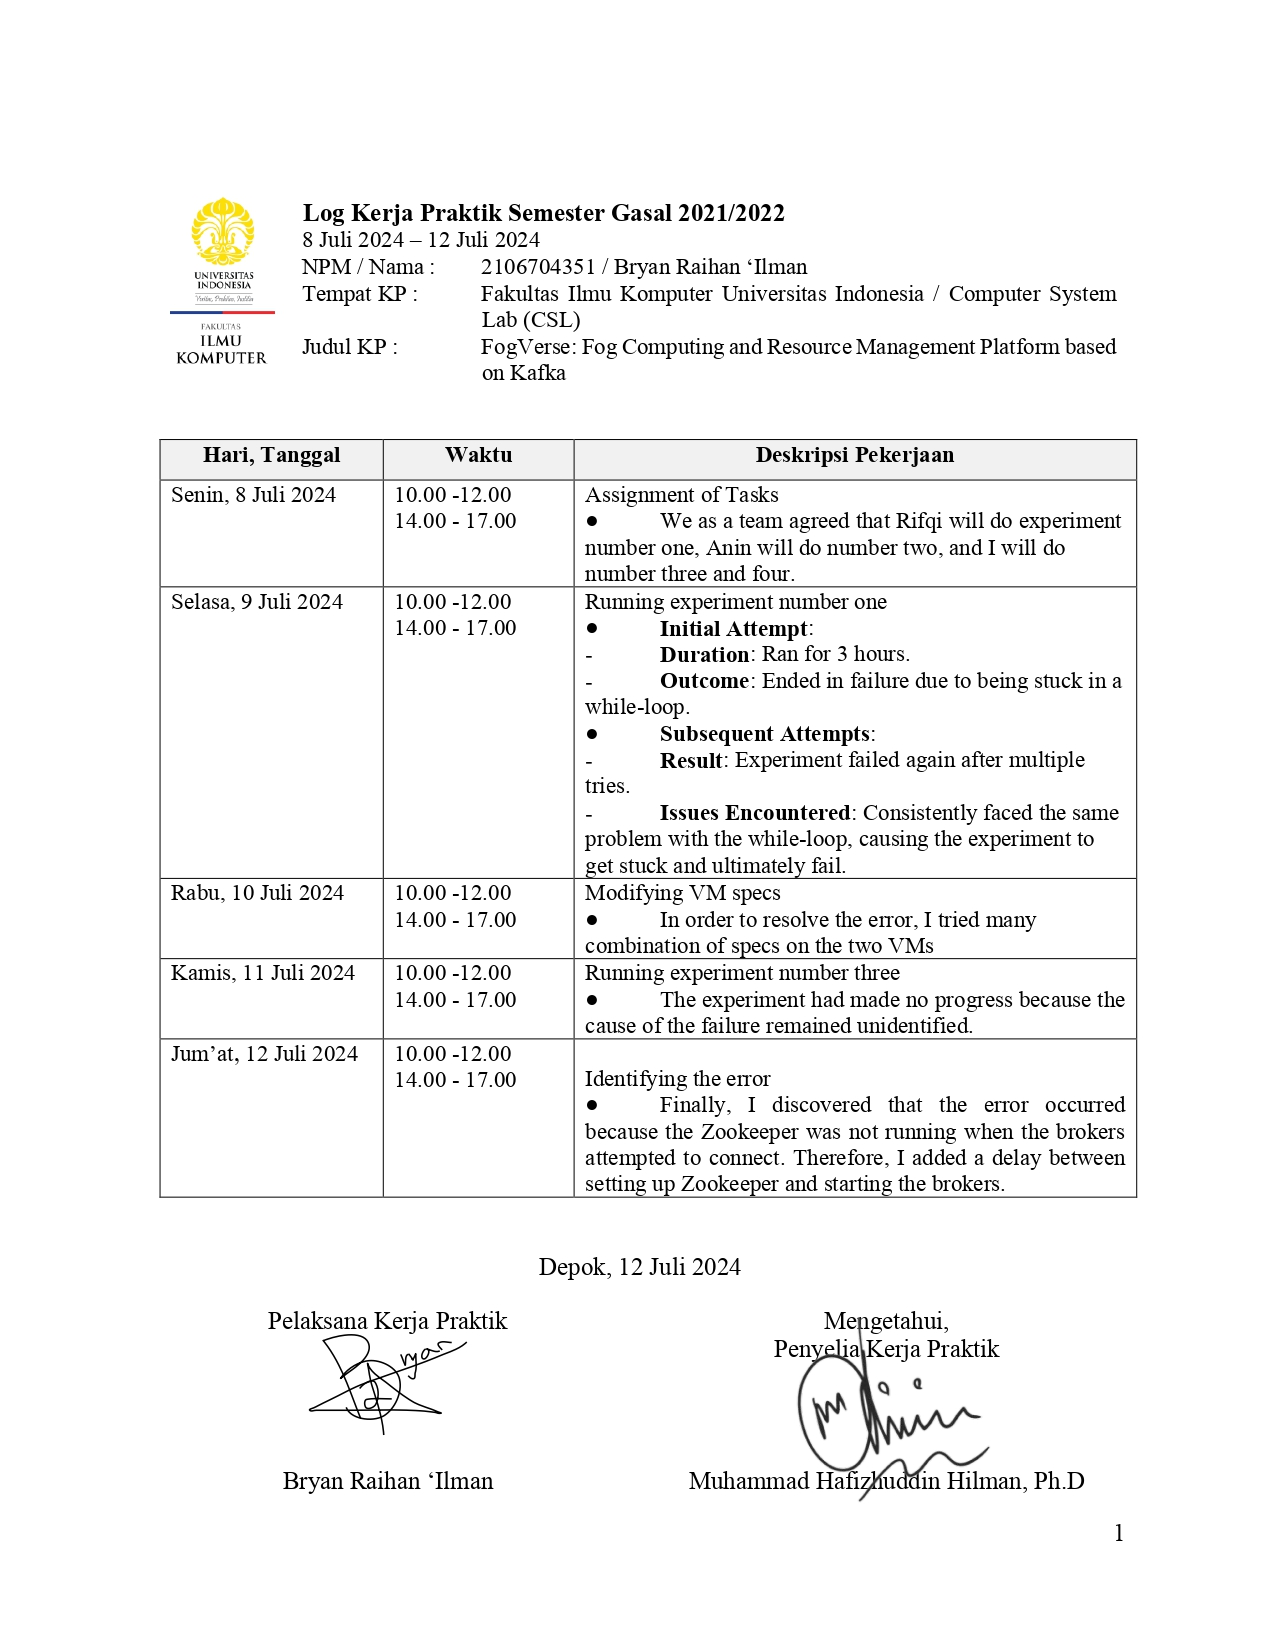
\includegraphics[width=1\textwidth]{assets/pics/Log-6-CSL-Bryan Raihan Ilman-0001.jpg}

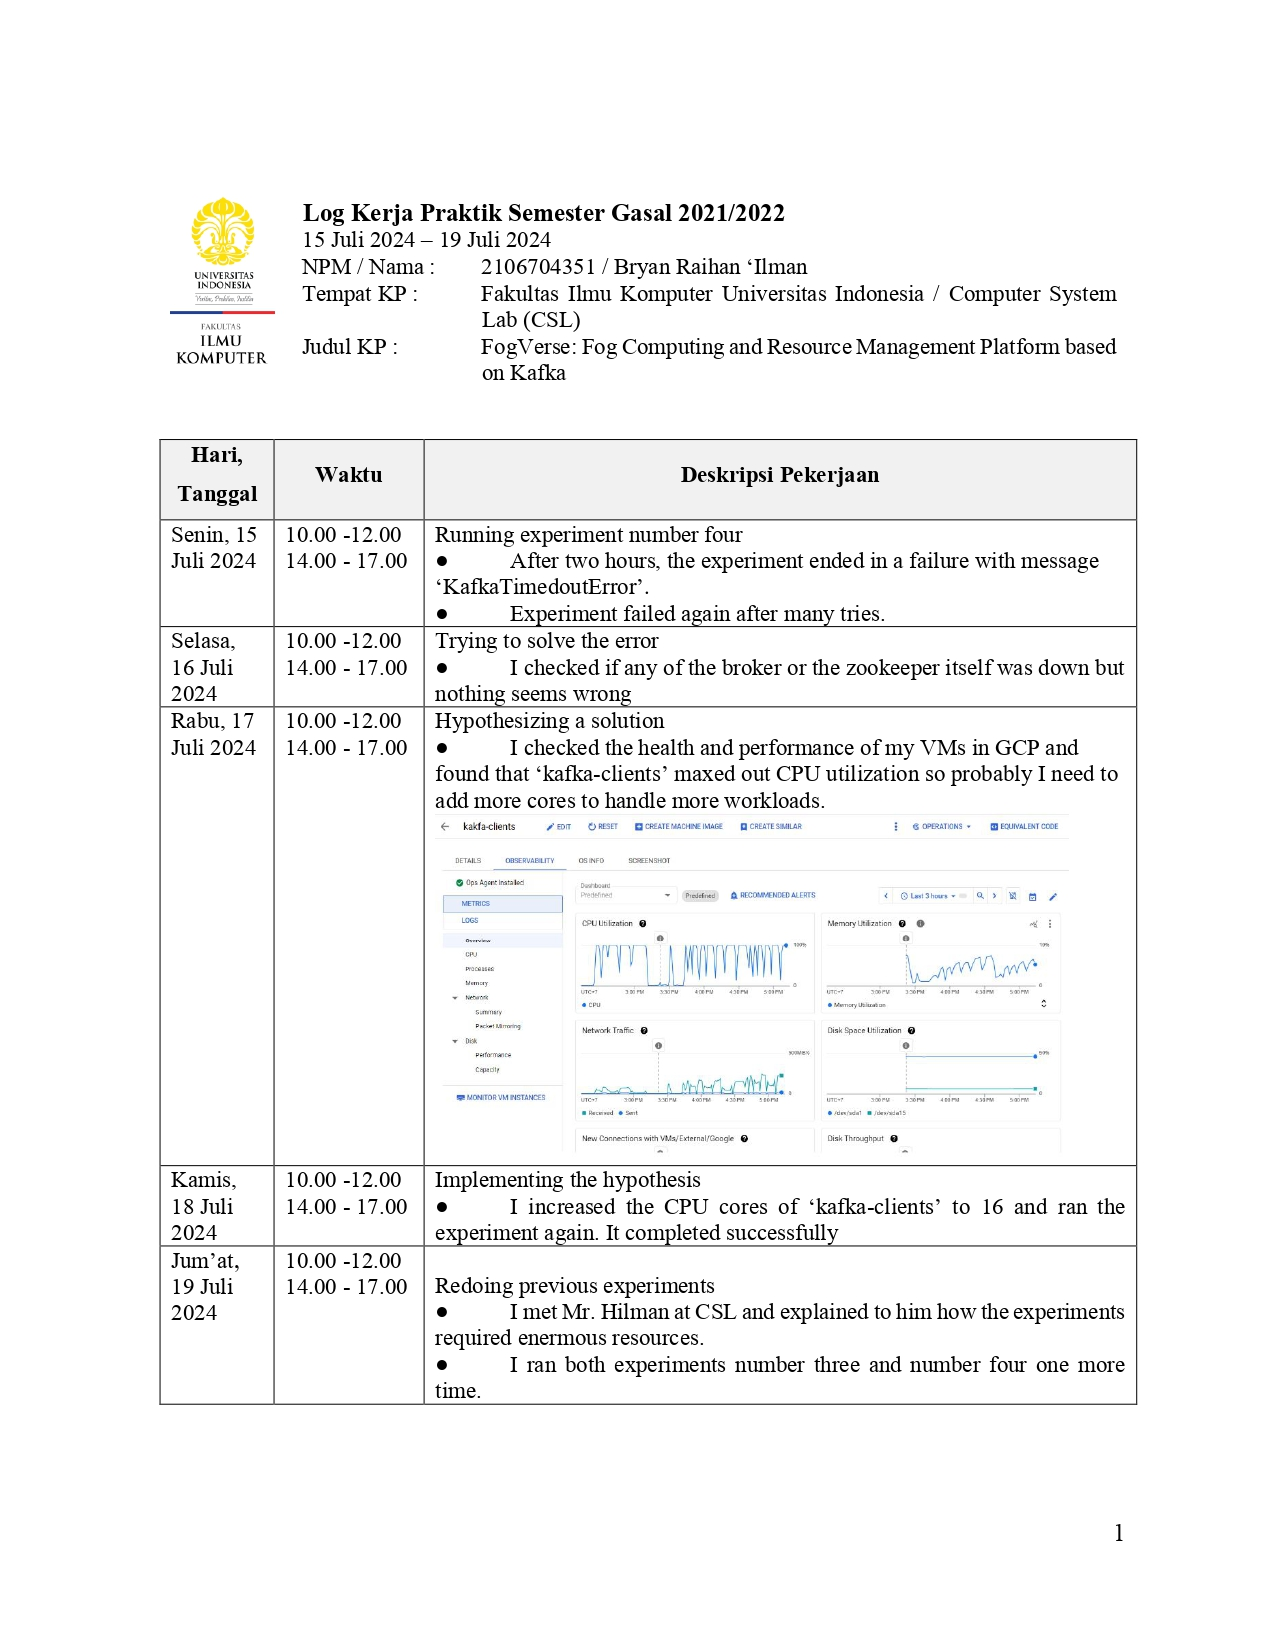
\includegraphics[width=1\textwidth]{assets/pics/Log-7-CSL-Bryan Raihan Ilman-0001.jpg}

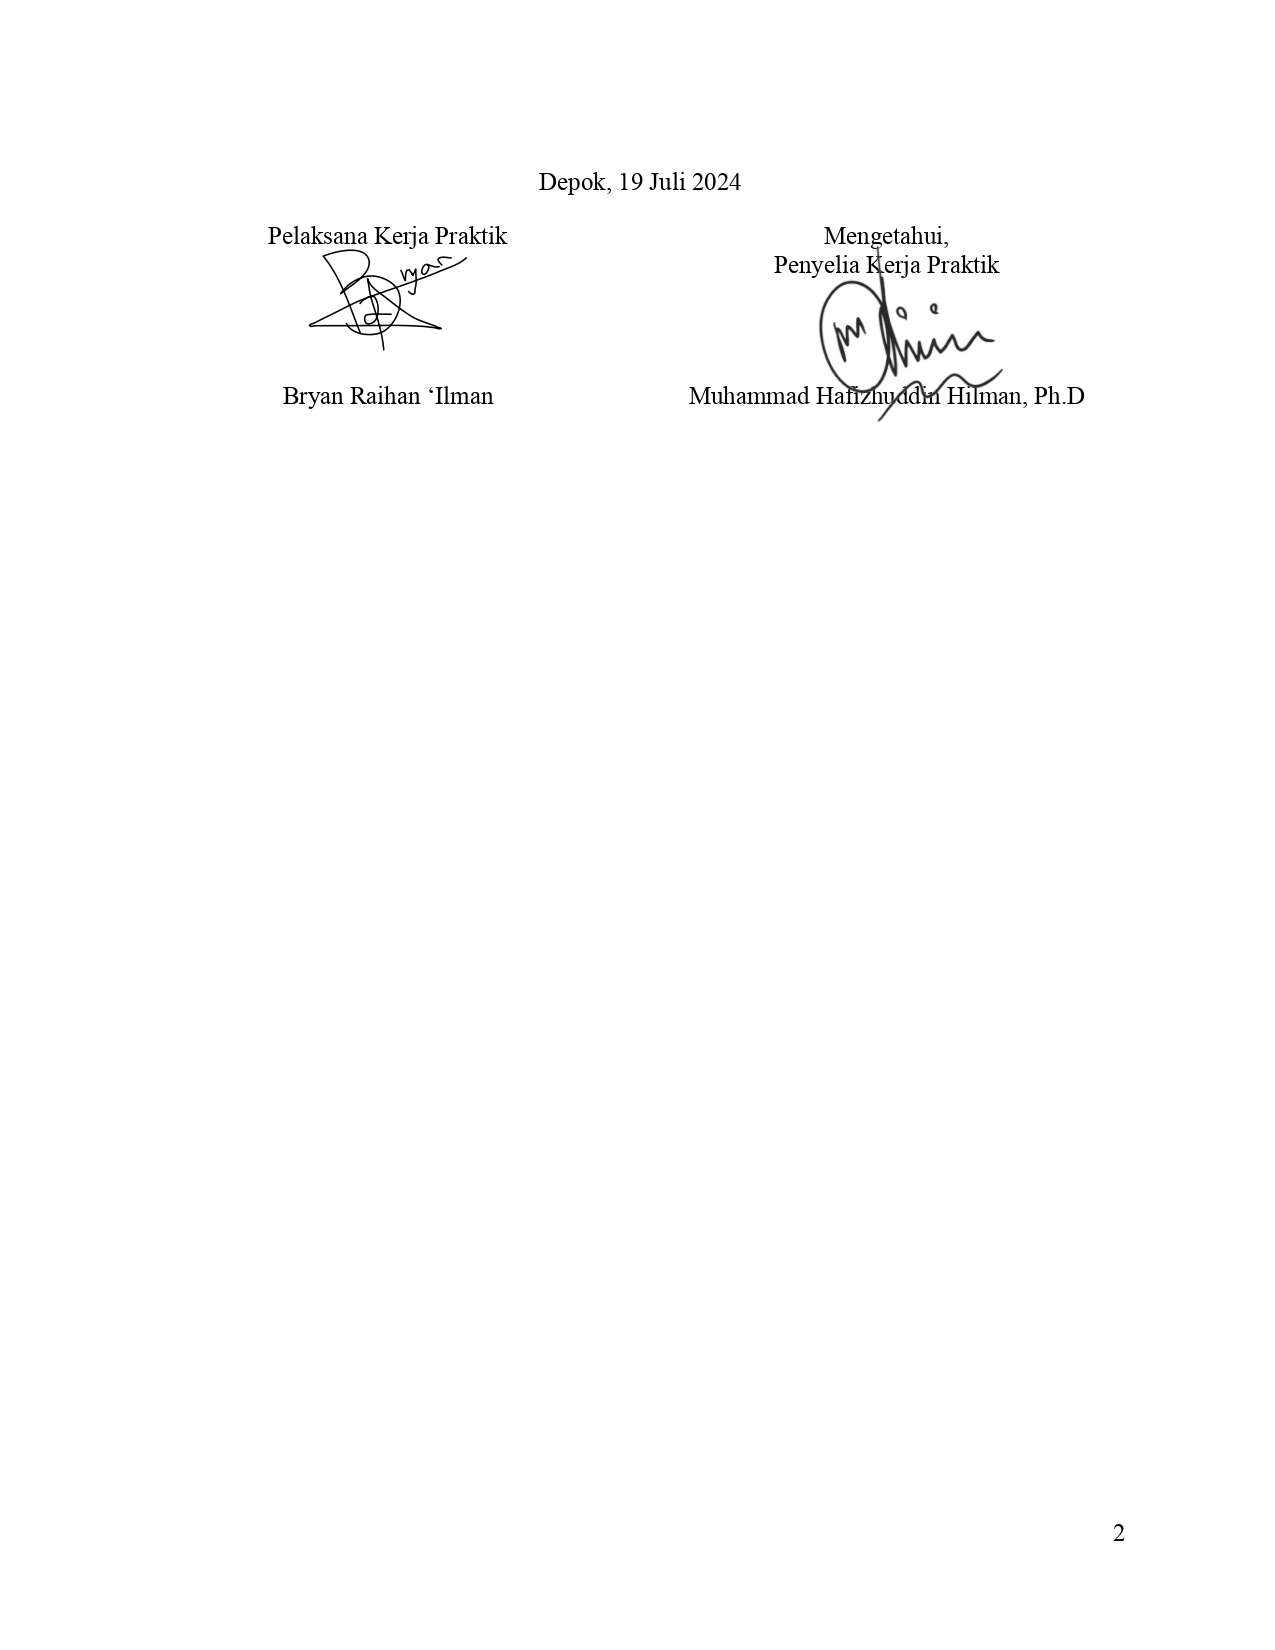
\includegraphics[width=1\textwidth]{assets/pics/Log-7-CSL-Bryan Raihan Ilman-0002.jpg}

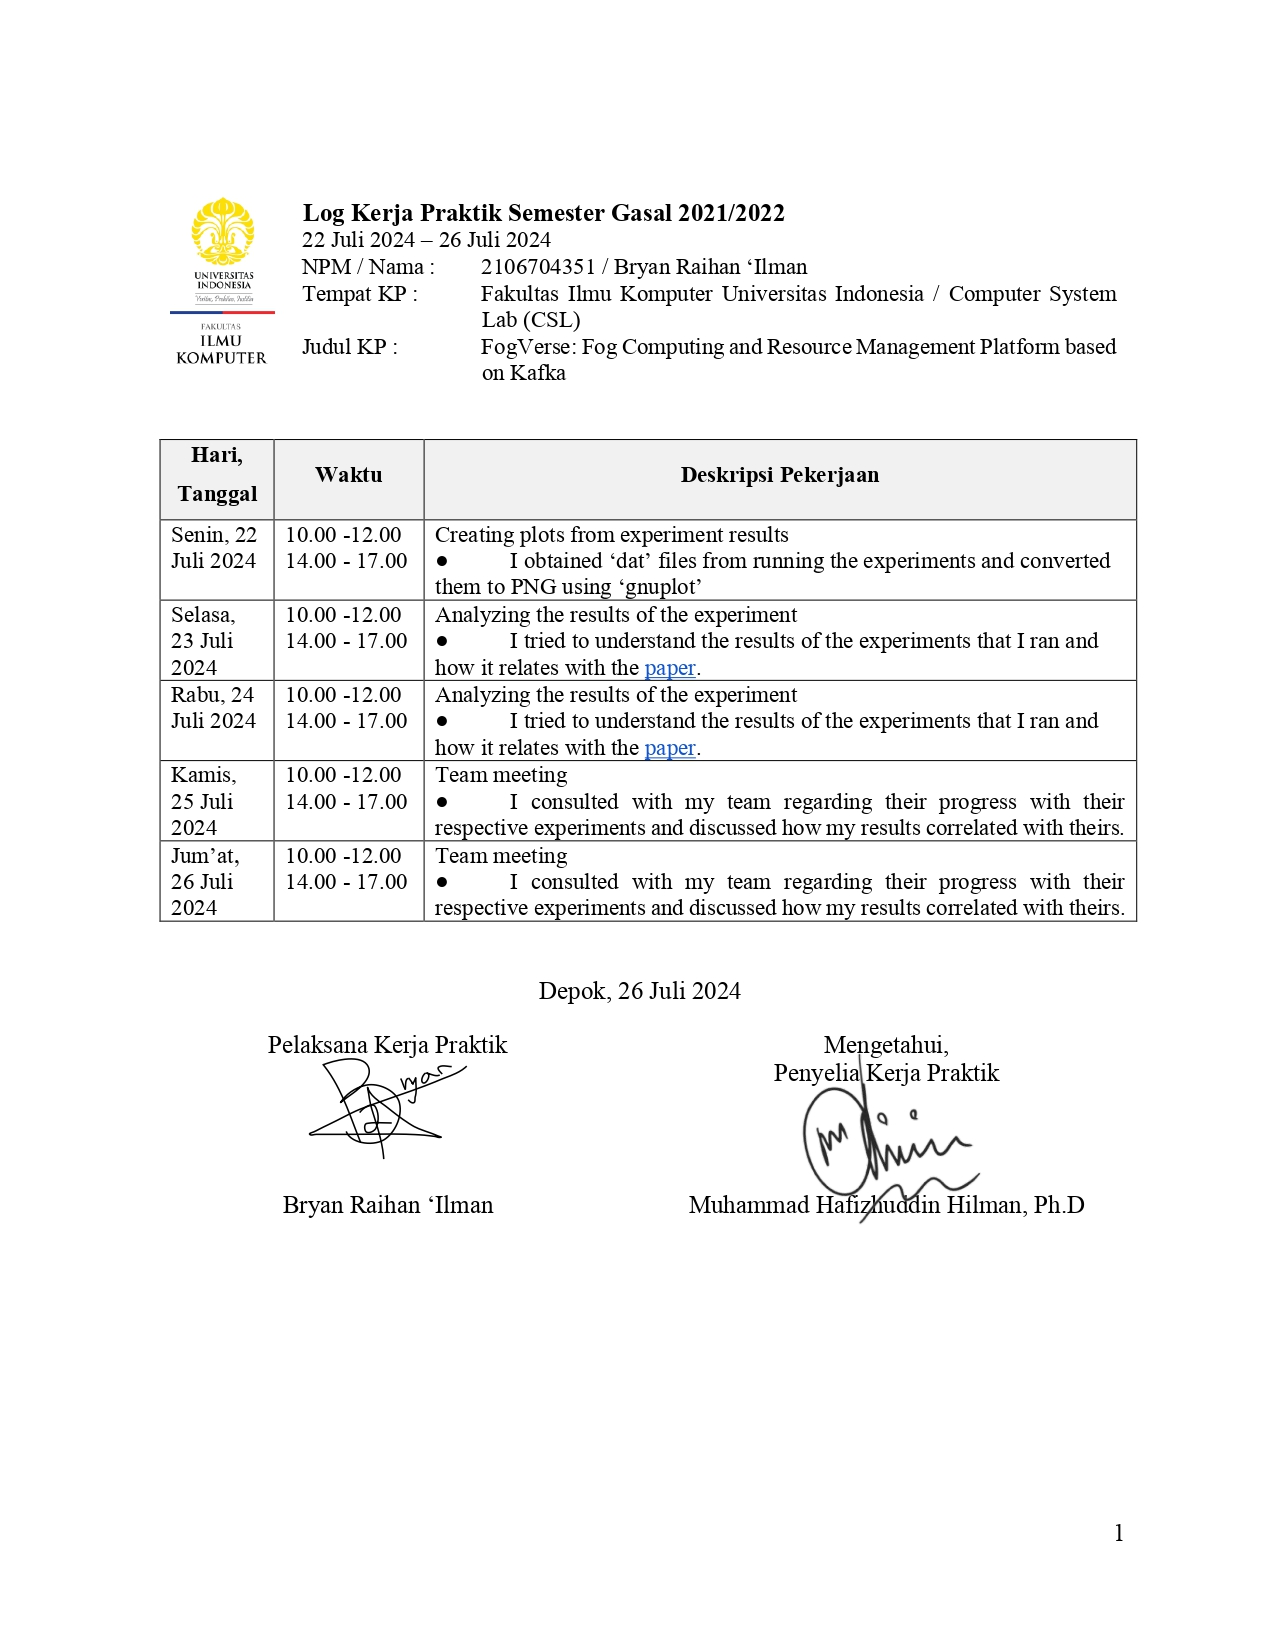
\includegraphics[width=1\textwidth]{assets/pics/Log-8-CSL-Bryan Raihan Ilman-0001.jpg}

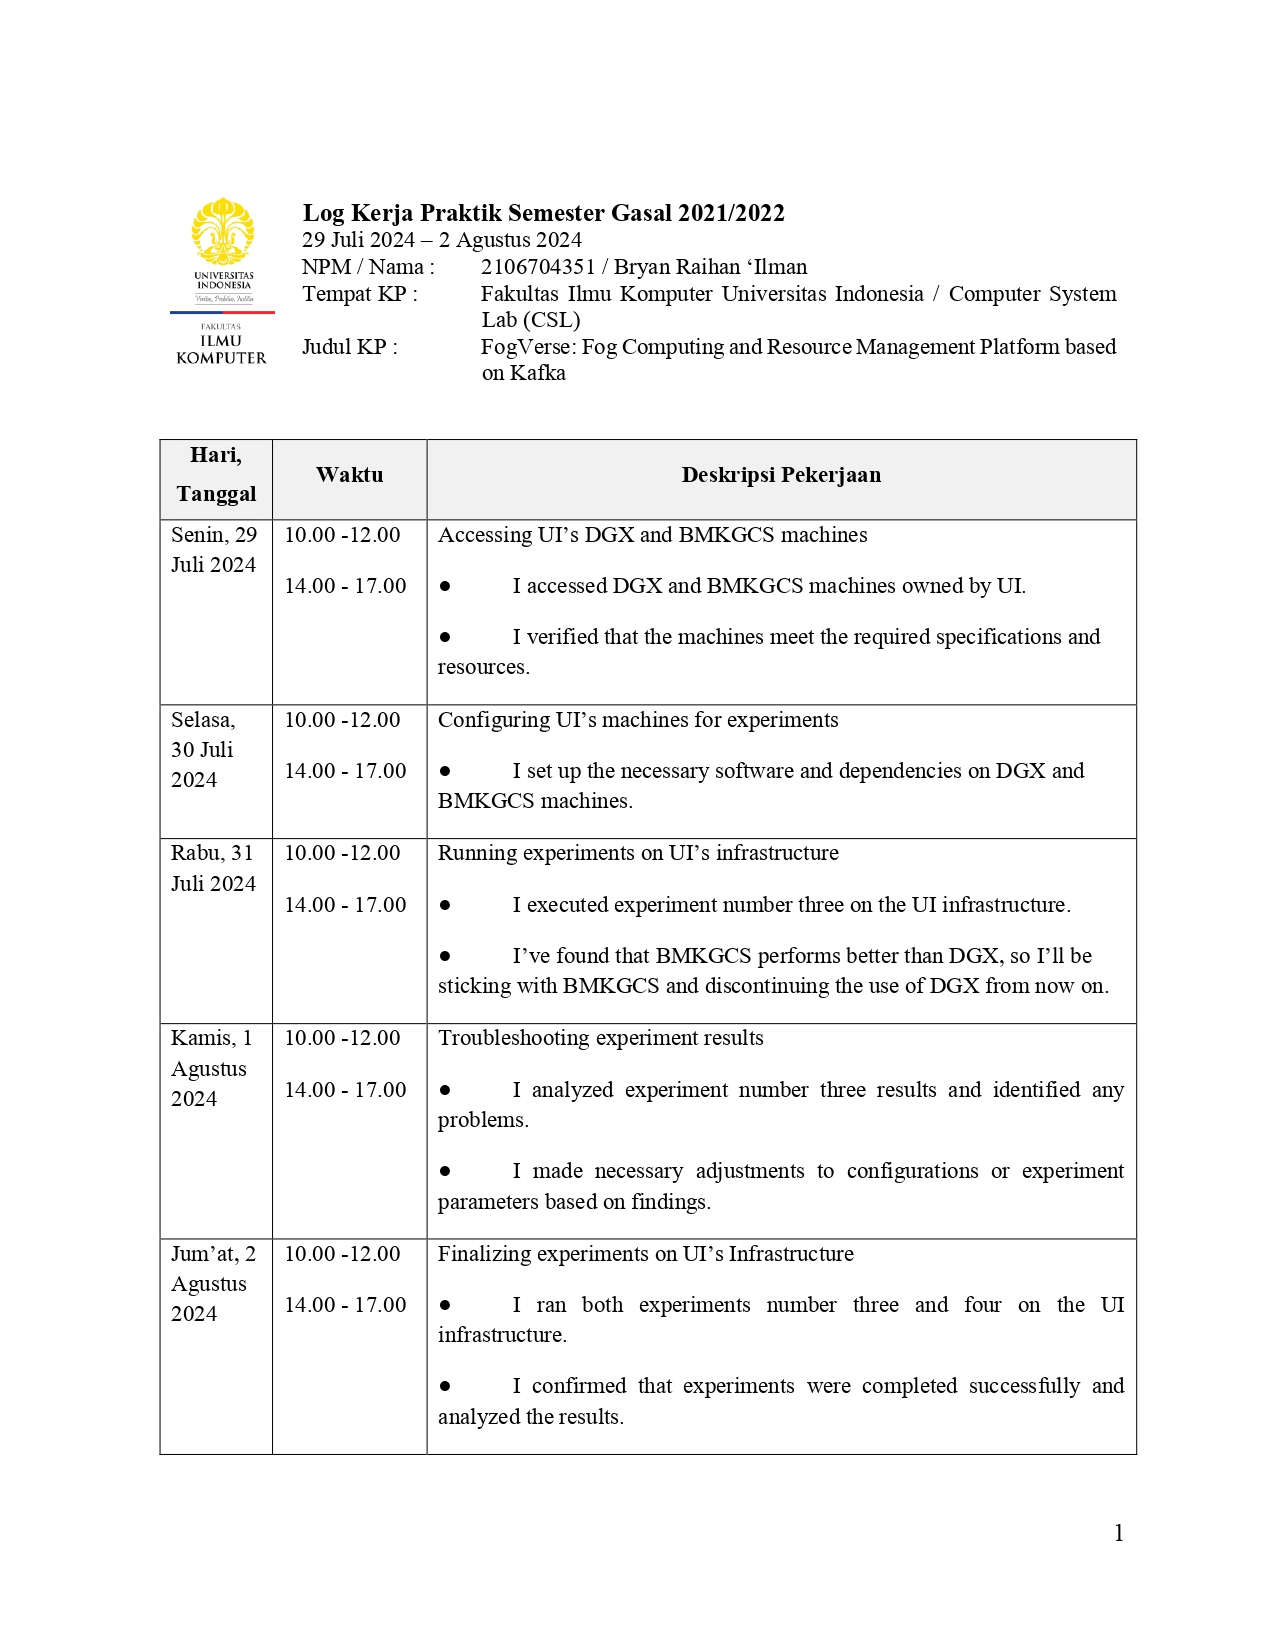
\includegraphics[width=1\textwidth]{assets/pics/Log-9-CSL-Bryan Raihan Ilman-0001.jpg}

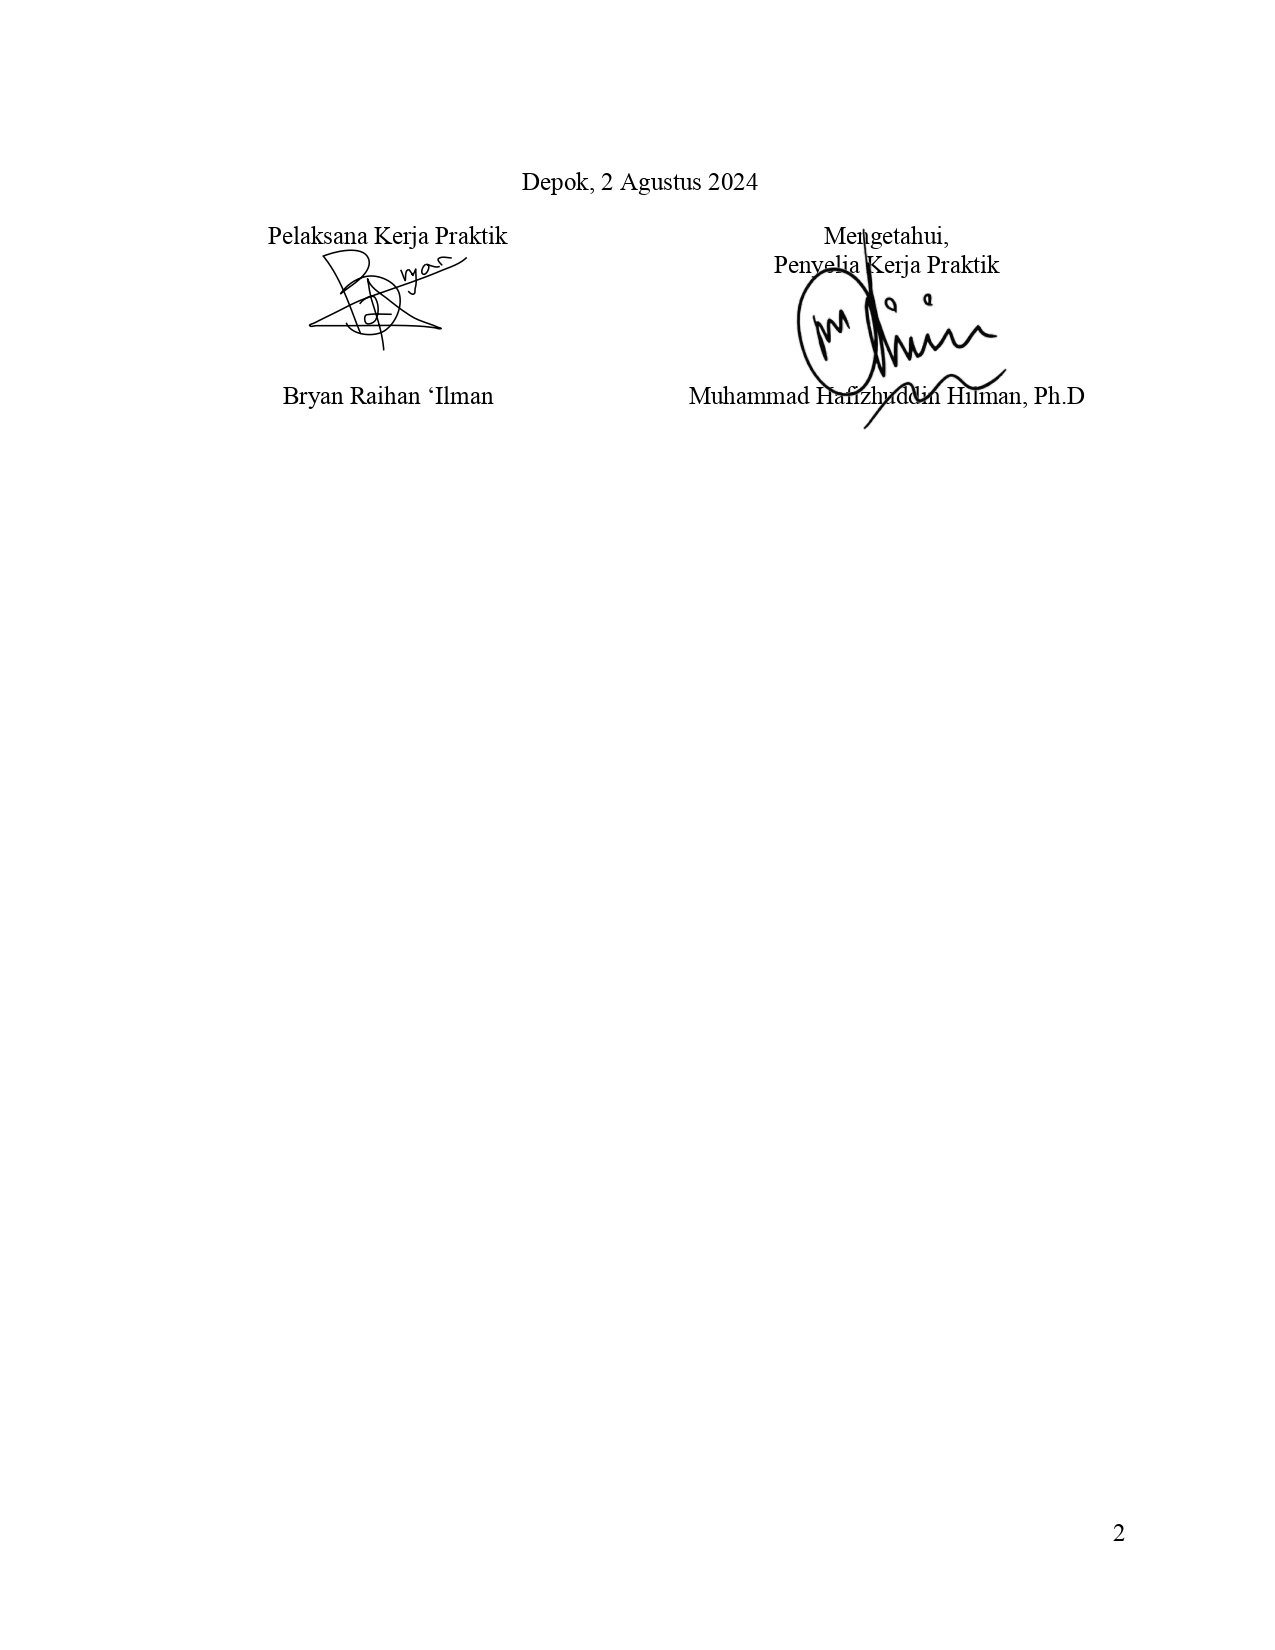
\includegraphics[width=1\textwidth]{assets/pics/Log-9-CSL-Bryan Raihan Ilman-0002.jpg}

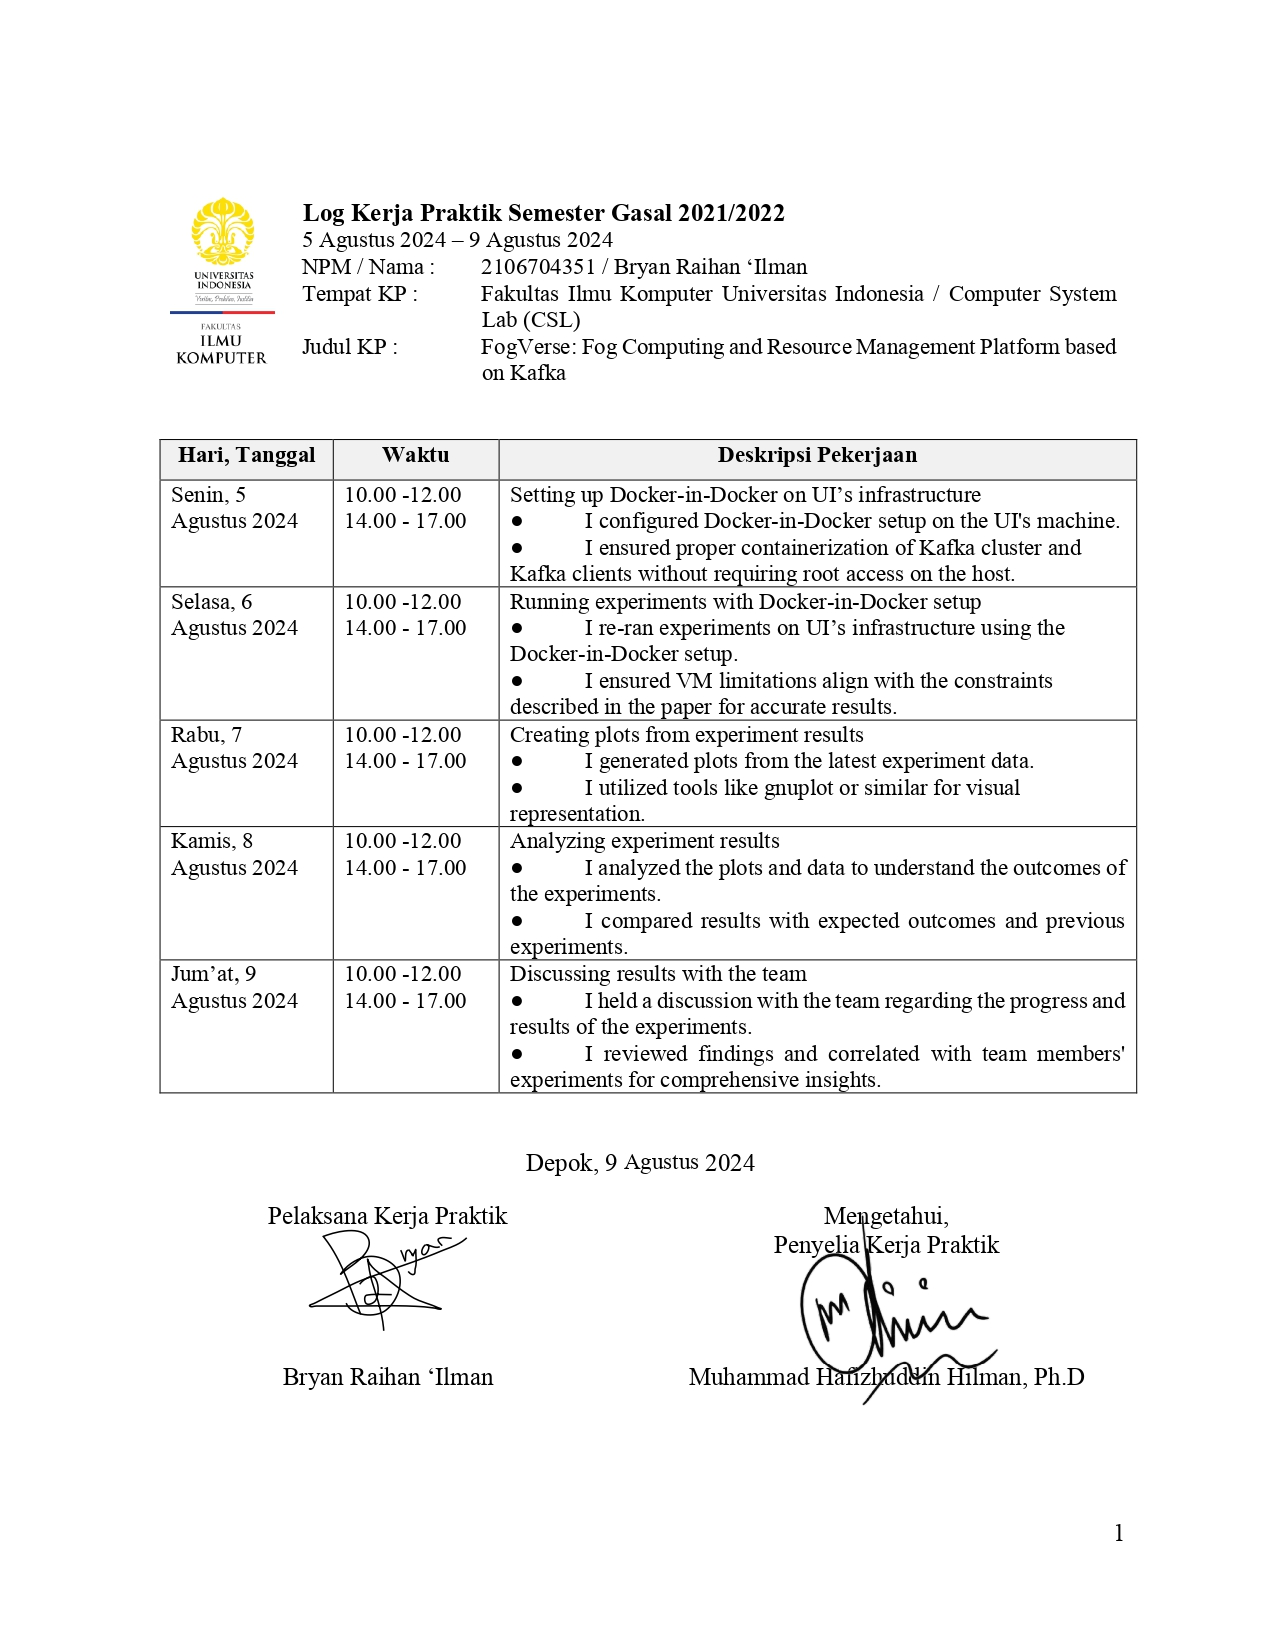
\includegraphics[width=1\textwidth]{assets/pics/Log-10-CSL-Bryan Raihan Ilman-0001.jpg}

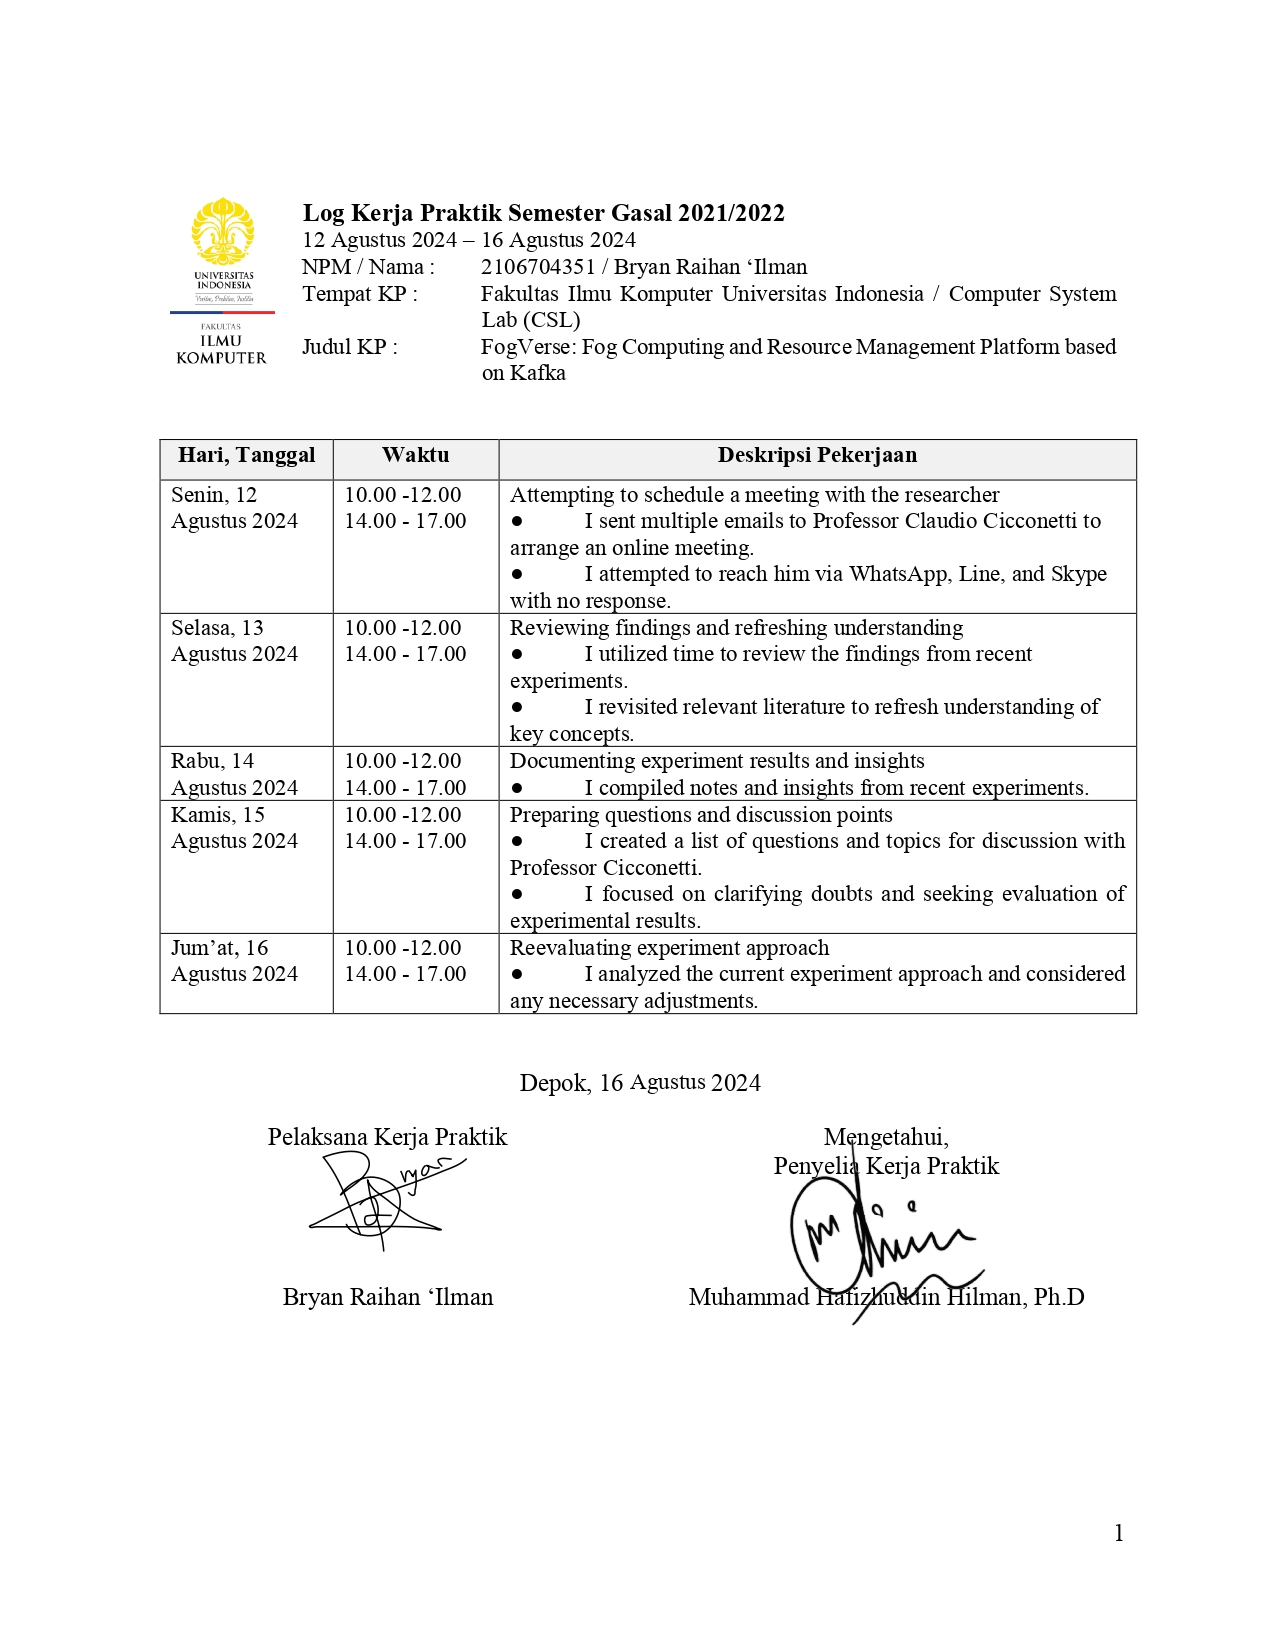
\includegraphics[width=1\textwidth]{assets/pics/Log-11-CSL-Bryan Raihan Ilman-0001.jpg}

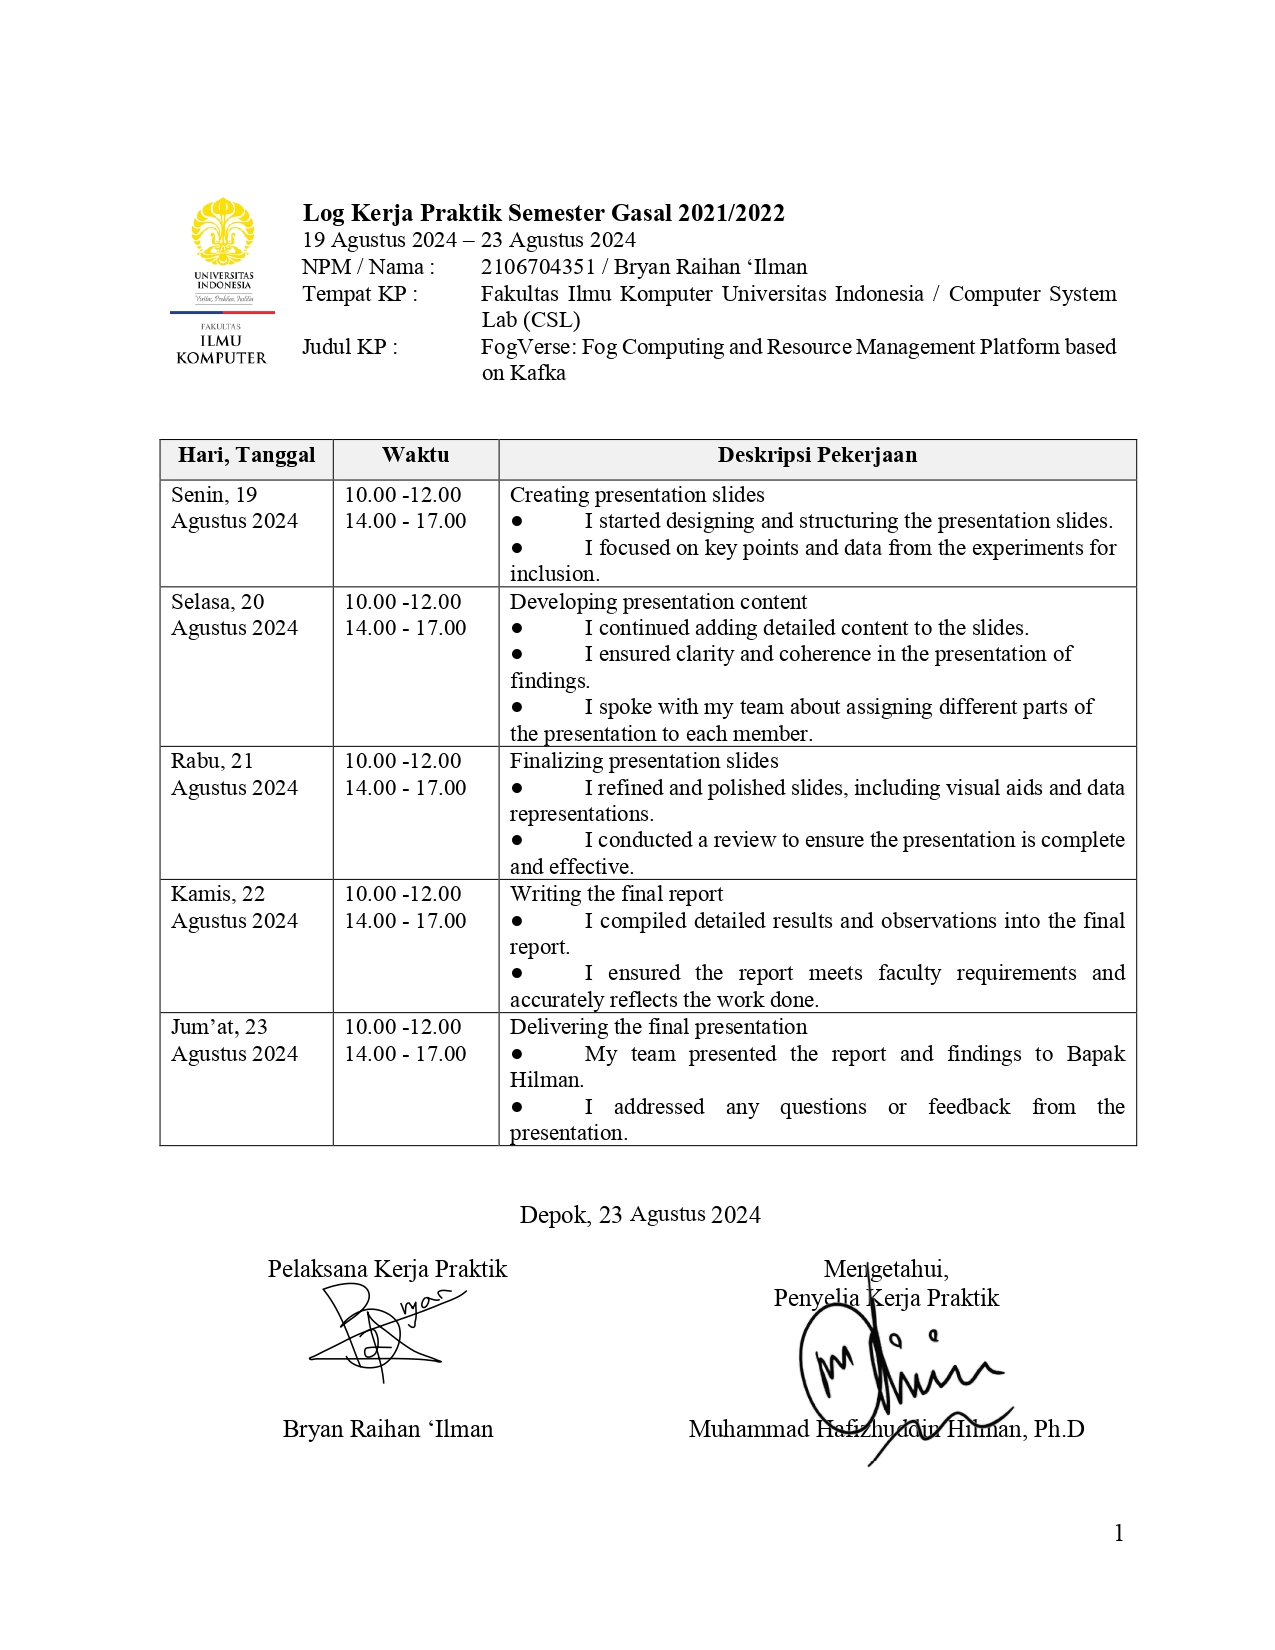
\includegraphics[width=1\textwidth]{assets/pics/Log-12-CSL-Bryan Raihan Ilman-0001.jpg}

\end{appendix}

\end{document}
